\documentclass[preprint,11pt]{elsarticle}
\usepackage[T1]{fontenc}
\usepackage{amsmath,amssymb,amsthm,mathtools}
\usepackage{booktabs,multirow,array}
\usepackage{graphicx}
\usepackage{algorithm}
\usepackage{algpseudocode}
\usepackage{xcolor}
\usepackage{enumitem}
\usepackage{url}
\biboptions{numbers,sort&compress}
\emergencystretch=2em

\newtheorem{theorem}{Theorem}
\newtheorem{proposition}{Proposition}
\newtheorem{lemma}{Lemma}
\newtheorem{corollary}{Corollary}
\theoremstyle{definition}
\newtheorem{definition}{Definition}
\newtheorem{assumption}{Assumption}
\newtheorem{example}{Example}
\theoremstyle{remark}
\newtheorem{remark}{Remark}

\newcommand{\rmin}{r^{\min}}
\newcommand{\rmax}{r^{\max}}
\newcommand{\E}{\mathbb{E}}
\newcommand{\ind}{\mathbf{1}}
\newcommand{\cK}{\mathcal{K}}
\newcommand{\cE}{\mathcal{E}}
\newcommand{\dem}{\mathrm{dem}}
\newcommand{\repay}{\textsc{Repay}}


\journal{Computer Networks}

\begin{document}

\begin{frontmatter}

\title{Priority Now, Payback Later: Online Capacity Allocation with Bounded Class Envy for Tiered Internet Access}

\author[buv]{Quang-Vinh Dang\corref{cor1}}
\ead{vinh.dq4@buv.edu.vn}
\ead[url]{https://orcid.org/0000-0002-3877-8024}
\cortext[cor1]{Corresponding author. ORCID: 0000-0002-3877-8024}
\affiliation[buv]{organization={British University Vietnam},
            city={Hung Yen},
            country={Vietnam}}

\begin{abstract}
An access point serves video calls and games, which need a modest rate every second, and downloads, which need volume and can wait, and sells free, premium and pay-as-you-go access on the same uncertain link.
Protecting real-time traffic during shortages is natural, but the class is in effect declared by the device, so rewarding the declaration ``real-time'' invites misreporting.
We propose \repay{}, an online rule that grants real-time priority on credit: a delay-tolerant device that is passed over accumulates a deficit that raises its priority and the price of real-time priority in its tier.
\repay{} is a drift-plus-penalty method with tier queues for business constraints and per-device deficit queues for fairness between classes.
We prove that every deficit, hence class envy, is bounded on every sample path; that for price-taking devices a misreport gains at most the bound per switch; and that utility is within $O(1/V)$ of an envy-free benchmark.
In simulations of a public hotspot, \repay{} serves $95\%$ of real-time slots against $82\%$ for proportional fairness, at a delay-tolerant throughput within $3\%$ of it, while the median misreporting device gains $1.3\%$, against $77\%$ to $170\%$ under uncapped class-aware rules.
On public Wi-Fi traces with rare real-time sessions, \repay{} gains $5$ to $14$ points over proportional fairness but priority rules serve $3$ to $15$ points more, at a class envy $10$ to $161$ times larger; a few devices on long stays exceed the incentive bound.
Of six further baselines from the literature, those that serve more real-time traffic reward misreporting.
\end{abstract}

\begin{keyword}
online resource allocation \sep network utility maximisation \sep drift-plus-penalty \sep fairness \sep envy-freeness \sep incentive compatibility \sep quality of service \sep access networks
\end{keyword}

\end{frontmatter}

\section{Introduction}\label{sec:intro}

An Internet access point is shared by devices whose needs differ in kind.
A video call needs a modest rate in every second and is worthless without it, although its picture quality can degrade.
An online game needs very little rate but needs it immediately.
A software update or a mailbox synchronisation needs volume and does not care when it arrives.
The operator of a home broadband service or of public Wi-Fi in a caf\'e, a metro station or an airport also sells different products on the same link: a free tier, a premium subscription, pay-as-you-go access.
And almost nothing is known in advance. Devices join and leave, sometimes dozens at once when a train arrives; demand switches on and off; the usable capacity moves with the backhaul and the radio channel.

When capacity is short, the natural reaction is to protect the real-time traffic and let the delay-tolerant traffic wait.
Doing this well runs into three difficulties at once.
The first is \emph{incentives}. With encrypted traffic the access point often cannot tell what an application is. When it relies on markings set by the device or by the application provider, the class of a flow is in effect declared; when it classifies traffic itself, an application can still shape its traffic to look like a call. We take the extreme case, in which the class is whatever the device says, as the working assumption: a rule that is robust there stays robust when a classifier narrows what can be claimed (Section~\ref{sec:related}).
If declaring ``real-time'' buys priority, every bulk transfer will declare it, and the protection disappears; we show that strict priority and standard utility-maximising schedulers both have this defect.
The second is \emph{fairness under churn}. Guarantees stated as long-run averages are of little use to a device that stays for four minutes.
The third is \emph{business constraints}: premium subscribers were promised a service level, pay-as-you-go traffic is revenue, and a venue that advertises free Wi-Fi must deliver some.

This paper proposes a rule that protects real-time traffic \emph{on credit}.
Real-time flows are served first during a shortage, and each elastic device that is passed over accumulates a deficit that records what it would have received had it claimed the real-time treatment.
The deficit acts in two directions: it raises the priority of the creditor, and it raises the price of further priority for the real-time flows of the same tier.
Elastic users care about volume more than about timing, so a device that stays long enough to be repaid loses little, while a real-time flow gets what it cares about, service now.
The two classes are thus offered different bundles that each prefers to the other's, and, for price-taking devices that stay long enough, telling the truth becomes approximately the best policy without any payment changing hands.

Credit-based sharing is not a new idea; it underlies recent resource managers and ``karma'' economies (Section~\ref{sec:related}).
What we add is a formulation of it inside online constrained optimisation, for service classes that differ in the shape of their utilities and for a population that changes continuously, together with guarantees that hold per device.

\paragraph{Contributions.}
\begin{enumerate}[leftmargin=*,itemsep=2pt]
\item \emph{Model.} We formulate online capacity allocation with unknown arrivals, departures, demands and capacity, three service classes, three commercial tiers with long-run business constraints, and a volume-based notion of \emph{class envy} that captures the temptation to misreport (Section~\ref{sec:model}).
\item \emph{Algorithm.} \repay{} is a drift-plus-penalty rule in which tier-level virtual queues persist across churn and per-device deficit queues are created at arrival. The per-slot problem is made concave by a perspective reformulation and an affine majorant, and is solved exactly by bisection, each step being linear in the number of devices (Section~\ref{sec:algorithm}).
\item \emph{Deterministic envy bound.} On every sample path, including adversarial ones, each deficit is at most $V w_g\eta_k+\rmax_k$. Hence the class envy of every elastic device over every window of its sojourn is bounded by a constant, that does not depend on the number of devices, on the churn, or on the tier prices (Theorem~\ref{thm:bound}).
\item \emph{Incentives.} For price-taking devices the gain in volume from a static misreport is at most this constant, and the gain collected while posing as real-time under a switching strategy is at most the constant times the number of switches; a bound on envy cannot control declarations that change in every slot, which motivates a hold-down on class changes (Theorems~\ref{thm:static}--\ref{thm:dynamic}, Proposition~\ref{prop:commit}). These statements assume price-taking devices and are informative for long stays; we test them against exact deviations in simulation, including in very small markets.
\item \emph{Utility.} For an arbitrary exogenous population process with exogenous demand caps and capacity that is conditionally independent given the population, the time-average utility of the fluid allocation is at most $O(1/V)$ below a benchmark of stationary policies that meet the business constraints in every population state and are class-envy-free in expectation; the violation of the business constraints is $O(\sqrt{V/T})$ in expectation and vanishes almost surely (Theorem~\ref{thm:opt}).
\item \emph{Evaluation.} In simulations of a public hotspot and a home network we compare \repay{} with proportional fairness, weighted fair queueing, strict priority, plain drift-plus-penalty, a Karma-style credit scheduler, strict priority with a capacity cap, and adaptations of six further schedulers and fair-division rules, both when devices are truthful and when they respond strategically, on synthetic traces with varied traffic mixes and population sizes and in three trace-driven scenarios built from public Wi-Fi session logs and mobile throughput logs (Section~\ref{sec:experiments}).
\end{enumerate}

We also state what the approach does not do. It is not the best rule on average performance: in our simulations strict priority with a cap on the real-time share that suits the traffic mix serves about as many real-time slots at a higher elastic rate, and in a trace-driven scenario with little real-time traffic the priority rules serve up to $15$ points more real-time slots; what \repay{} offers instead is a bound for every device that does not depend on the traffic mix. On those traces our default configuration is also not the best one: the variant without the debt price at a smaller $V$ serves more real-time slots with less envy and a similar incentive to misreport. When capacity is short permanently, bounded envy forces real-time flows to be rationed; the benefit of \repay{} lies in transient shortages. The incentive guarantee is approximate: it assumes price-taking devices, it is a constant per stay and therefore weak for short visits, and in our simulations between a quarter and two thirds of the devices still gain a small amount by misreporting, depending on the scenario, and a few of them more than the bound, mostly free devices on long stays and one in a thin premium tier by a factor of twelve. It also presupposes that demand is measured by the access point, which is natural for downlink traffic only.
Section~\ref{sec:discussion} discusses these limits.


\section{Related work}\label{sec:related}

\paragraph{Utility maximisation and fairness.}
Network utility maximisation and proportional fairness go back to \citet{kelly1998rate}, and the $\alpha$-fair family to \citet{mo2000fair}; \citet{lan2010axiomatic} derive such families from axioms and \citet{bertsimas2011price} quantify the efficiency that fairness costs.
The distinction between elastic and real-time applications is due to \citet{shenker1995fundamental}, and rate control with non-concave, inelastic utilities was studied by \citet{lee2005nonconvex} and \citet{hande2007distributed}.
Weighted fair queueing and its practical approximations \citep{parekh1993generalized,shreedhar1996efficient} are the classical mechanisms, and airtime-fair scheduling has been built for commodity Wi-Fi access points \citep{hoiland2017ending}.
These frameworks take the set of flows and their classes as given.
Closer to our setting, \citet{sisalem2023enabling} contrast fairness in every slot with fairness over the horizon and show that vanishing regret for the latter is impossible against an unrestricted adversary, and \citet{elazzouni2020deadline} treat online, deadline-constrained allocation with fairness.

\paragraph{Classification and queue management in deployed networks.}
Operators do not rely on declarations alone.
Wi-Fi access categories are selected from the Diffserv marking of a packet \citep{rfc8325}, which for uplink traffic is set by the device and for downlink traffic by whoever sits upstream; many networks reset it at their boundary and classify traffic themselves, increasingly with learned classifiers that work on encrypted flows \citep{rezaei2019deep}.
A second line of practice avoids classes altogether: flow queueing with active queue management \citep{rfc8290,hoiland2018cake} isolates flows and gives sparse flows low delay without asking what they are, and L4S \citep{rfc9330} lets a flow ask for low queueing delay on the condition that it responds to congestion marks, which is designed to reduce the incentive to misdeclare, since the low-delay queue is designed to carry no throughput advantage, although the service relies on self-restraint.
These mechanisms control delay at the scale of packets and share the rate equally among flows or hosts, so on the time scale of our model we expect them to behave like the class-blind baseline \textsc{PF} (we did not simulate a flow-queueing baseline): when the equal share falls below what a call needs, the call fails.
A classifier is complementary to our rule. Its output can replace the declaration, and since every classifier errs and can be imitated, a rule under which being taken for real-time is not worth much limits the damage of its errors; we do not model classification errors here.

\paragraph{Stochastic network optimisation and constrained online learning.}
Our algorithm belongs to the drift-plus-penalty family \citep{georgiadis2006resource,neely2010stochastic}, which builds on the primal--dual and queue-based methods of \citet{stolyar2005maximizing}, \citet{eryilmaz2007fair} and \citet{neely2008fairness}.
Deterministic bounds on virtual queues are a known device in this literature, for example for worst-case delay \citep{neely2011worstcase}; we do not claim the technique, only its use for a per-device fairness property.
\citet{jaramillo2011elastic} combine elastic and real-time traffic in one Lyapunov scheme with per-flow deficit counters; there the deficit protects the delivery ratio of real-time flows, whereas ours protects elastic devices \emph{against} real-time priority, and their flow set is fixed.
Online convex optimisation with long-term constraints \citep{mahdavi2012trading,yu2017online,yu2019low} gives regret and violation guarantees for aggregate constraints, and online allocation by dual descent \citep{balseiro2023best,balseiro2025regularized} gives regret and competitive-ratio guarantees under resource constraints; recent work relaxes Slater's condition and handles time-varying constraints \citep{yu2026slater,sarkar2026geometric,abdullah2026dynamic}.
In these models the constrained quantities are properties of the system, not of agents who come and go.
\citet{sinclair2021sequential} characterise the envy--efficiency trade-off when individuals arrive online, each for a single round, and \citet{li2020combinatorial} use virtual queues to guarantee minimum service to arms that may be unavailable.
To our knowledge, and within the literature we searched (the venues and preprint servers of networking, optimisation, operations research and algorithmic game theory up to November 2026), there is no drift-plus-penalty or constrained-online-learning result with guarantees per agent over a finite sojourn, nor one that enforces envy constraints through virtual queues.

\paragraph{Pricing and screening by delay.}
That delay can separate customer types is classical in queueing economics: \citet{mendelson1990optimal} price priorities incentive-compatibly and \citet{afeche2013incentive} shows that deliberately delaying patient customers can be optimal.
Paris Metro Pricing applies the idea to networks \citep{odlyzko1999paris}, and \citet{sen2013survey} survey time- and usage-dependent data pricing.
The economics of public Wi-Fi, including free access funded by advertising, is studied by \citet{yu2017public}, and the pricing of Wi-Fi access points by \citet{musacchio2006wifi}; \citet{johari2004efficiency} bound the efficiency loss when users of a shared link anticipate prices.
Most of these screen with payments or prices.
\repay{} screens with time alone: the elastic class is offered more volume later, and the tier, which is where money enters, is taken as fixed.

\paragraph{Allocation without money and credit mechanisms.}
A large literature allocates shared resources fairly without payments, starting with dominant resource fairness \citep{ghodsi2011dominant} and its dynamic extensions \citep{kash2014no,freeman2018dynamic,fikioris2021incentives}; \citet{cole2013mechanism} design truthful mechanisms without payments, and \citet{gorokh2021monetary} obtain approximate truthfulness, with gains from misreporting that vanish over time, through artificial currencies.
The idea that underlies our deficit queues, serving urgent demand now and repaying the others later, is \emph{not} new.
Karma \citep{vuppalapati2023karma} implements it with credits for a single elastic resource and proves online strategy-proofness; \citet{le2019bopf} give latency-sensitive queues bounded priority over throughput-sensitive ones in clusters; karma economies allocate road and charging capacity among agents with heterogeneous urgency \citep{elokda2024karma,elokda2025carma,elokda2026ev}; \citet{wong2013myob} distribute credits across home gateways of an ISP; and \citet{zahedi2026credit} formalise credit fairness and prove that no mechanism is at once anonymous, strategy-proof, credit-fair and Pareto efficient.
Related guarantees for repeated allocation without money appear in \citet{balseiro2019nomoney}, \citet{banerjee2023pseudo}, \citet{fikioris2025dmmf} and \citet{lin2026spec}, envy that grows sublinearly in the horizon in \citet{benade2018envy}, and a deficit-based rule with anytime fairness bounds in \citet{kahana2026perpetual}.
Most of these works consider agents of a single kind, who differ in demand or urgency but not in the shape of their utility (\citet{le2019bopf} distinguish two job classes, and the karma models let urgency vary), a fixed or heuristically handled population, and no long-run constraints of the operator.
Our contribution is narrower and complementary: we place the repayment idea inside a constrained stochastic optimisation with heterogeneous service classes and commercial tiers, and obtain a sample-path bound per device that is unaffected by churn.
Consistent with the impossibility result of \citet{zahedi2026credit}, our incentive guarantee is approximate; it uses the price-taking hypothesis that underlies the large-market notion of \citet{azevedo2019strategy}, without establishing a large-market limit.
\citet{dai2025efficiency} show, for indivisible resources, that strategic agents can manipulate the dual variables of primal--dual allocation rules, and they counter this with payments combined with lazy dual updates and random exploration; our price-taking hypothesis sets this channel aside in the theory, and we measure it in the experiments.

\paragraph{Robust and stochastic optimisation.}
A different way to face uncertainty is to hedge against it at design time: robust routing under demand uncertainty \citep{benameur2005routing}, robust optimisation with budgeted uncertainty \citep{bertsimas2004price}, robust network enhancement \citep{rezaei2026robust}, distributionally robust optimisation \citep{mohajerin2018data}, and stochastic programming for slice provisioning \citep{gholami2023mobile}.
\citet{boyd2007dynamic} consider multi-period utility maximisation with delivery contracts that couple rates across time, the closest analogue of our long-run business constraints.
These approaches fix the population and optimise capacity or routing decisions; they are complementary to an online rule that reacts slot by slot and needs no uncertainty set.

\begin{table}[t]
\centering
\caption{Features covered by representative approaches. ``RT'' means that real-time classes are modelled as such; ``IC'' that class or demand reports are strategic; a dot means partially. For \repay{} the fairness guarantee is bounded class envy for the implemented allocation, the constraint guarantee is for the fluid allocation, and ``approximate'' means for price-taking devices.}
\label{tab:related}
\small
\resizebox{\linewidth}{!}{\begin{tabular}{@{}lccccc@{}}
\toprule
 & churn & RT classes & tiers / constraints & fairness & IC without money\\
\midrule
NUM, WFQ \citep{kelly1998rate,parekh1993generalized} & -- & -- & $\cdot$ & \checkmark & --\\
Inelastic NUM \citep{lee2005nonconvex,hande2007distributed} & -- & \checkmark & -- & $\cdot$ & --\\
Drift-plus-penalty \citep{neely2010stochastic,jaramillo2011elastic} & -- & \checkmark & \checkmark & \checkmark & --\\
Constrained online learning \citep{yu2017online,balseiro2025regularized} & -- & -- & \checkmark & $\cdot$ & --\\
Priority pricing \citep{mendelson1990optimal,afeche2013incentive} & -- & \checkmark & $\cdot$ & -- & -- (payments)\\
Credit mechanisms \citep{vuppalapati2023karma,zahedi2026credit} & $\cdot$ & -- & -- & \checkmark & $\cdot$\\
\repay{} (this paper) & \checkmark & \checkmark & \checkmark & \checkmark & approximate\\
\bottomrule
\end{tabular}}
\end{table}


\section{Model and problem statement}\label{sec:model}

\paragraph{Time, capacity and population.}
Time is slotted, $t=1,2,\dots$; we think of a slot as one second and measure rates in Mbit/s.
An access point (a home gateway or a public hotspot) has capacity $C_t>0$ in slot $t$.
The set of active devices changes from slot to slot as devices arrive and leave.
At the start of slot $t$ the operator observes $C_t$ and the data of the currently active devices; it has no information, not even distributional, about later slots.

\paragraph{Tiers.}
Every device belongs to a commercial tier $g\in\{F,P,Y\}$: free, premium, or pay-as-you-go (PAYG).
The tier is the billing identity of the subscriber. It is verified by the operator and cannot be misreported.
Tier $g$ carries a weight $w_g>0$ that expresses how much the operator values a unit of utility delivered to that tier.

\paragraph{Service classes.}
A device declares a service class, which the operator cannot verify.
Class $E$ (elastic) stands for delay-tolerant traffic such as e-mail, backups and downloads.
The real-time (RT) classes $k\in\cK=\{\mathrm{v},\mathrm{g}\}$ are interactive video ($\mathrm{v}$) and online gaming ($\mathrm{g}$).

An RT flow of class $k$ is useful only if it receives a rate in $[\rmin_k,\rmax_k]$ in the current slot, where $0<\rmin_k\le\rmax_k$.
A rate below $\rmin_k$ makes the slot worthless, and rate above $\rmax_k$ brings nothing.
Its per-slot utility is $u_k(z)$, bounded, nondecreasing and concave on $[\rmin_k,\rmax_k]$ (strictly concave if $\rmin_k<\rmax_k$) with $u_k(\rmin_k)>0$.
We use $u_{\mathrm{v}}(z)=1+\log(z/\rmin_{\mathrm{v}})$, which models a call whose quality degrades gracefully down to $\rmin_{\mathrm{v}}$, and a constant $u_{\mathrm{g}}\equiv 1$ at a fixed rate $\rmin_{\mathrm{g}}=\rmax_{\mathrm{g}}=r_{\mathrm{g}}$.
Let
\begin{equation}\label{eq:eta}
\eta_k=\max_{z\in[\rmin_k,\rmax_k]}\frac{u_k(z)}{z},
\end{equation}
the largest utility per unit of rate that a class-$k$ flow can generate; for both utilities above $\eta_k=u_k(\rmin_k)/\rmin_k=1/\rmin_k$.

An elastic device $i$ has a demand cap $d_{i,t}\ge 0$ in slot $t$: the smaller of its link rate and the traffic queued for it at the access point.
For downlink traffic both quantities are measured by the access point itself, so $d_{i,t}$ is \emph{verified}, not declared.
The deficit bound of Section~\ref{sec:envy} holds for arbitrary demand caps; the incentive and optimality results of Sections~\ref{sec:ic} and~\ref{sec:opt} additionally treat the caps as exogenous, as for a device with a standing backlog.
The device receives a rate $x_{i,t}\in[0,d_{i,t}]$.
What an elastic user cares about is how much data it gets, not when: its true preference is an arbitrary nondecreasing function of the cumulative volume $\sum_t x_{i,t}$ received during its sojourn.
The operator scores elastic service with the concave surrogate $w_g\,u(x)$, $u(x)=\log(1+x)$, which yields weighted proportional fairness among elastic devices; the analysis only uses that $u$ is strictly concave, differentiable and strictly increasing, so in principle any $\alpha$-fair utility $((1+x)^{1-\alpha}-1)/(1-\alpha)$ can be substituted, with the corresponding change in the closed form \eqref{eq:xresp} (our implementation and experiments use $\alpha=1$, and we have not checked the hypotheses of Proposition~\ref{prop:reverse} for other values).

\paragraph{Decisions.}
Let $n_{g,k,t}$ be the number of active flows of tier $g$ that declare class $k$.
For every nonempty group $(g,k)$ the operator chooses an admission fraction $a_{g,k,t}\in[0,1]$ and a common rate $z_{g,k,t}\in[\rmin_k,\rmax_k]$; a fraction $a$ of the flows is served at rate $z$ and the others are blocked in this slot.
We write $y_{g,k,t}=a_{g,k,t}z_{g,k,t}$ for the mean rate per flow.
The capacity constraint is
\begin{equation}\label{eq:cap}
\sum_{g,k} n_{g,k,t}\,y_{g,k,t}+\sum_{i\in\cE_t}x_{i,t}\le C_t ,
\end{equation}
where $\cE_t$ is the set of active devices that declare $E$.
The total rate of tier $g$ is $\rho_{g,t}=\sum_k n_{g,k,t}y_{g,k,t}+\sum_{i\in\cE_t:\,g_i=g}x_{i,t}$ and its demand is $\dem_{g,t}=\sum_k n_{g,k,t}\rmax_k+\sum_{i\in\cE_t:\,g_i=g}d_{i,t}$.
The paid tiers come with a \emph{committed rate} $c_g$ per device, the rate the product promises; the committed demand of tier $g$ is $\mathrm{com}_{g,t}=\sum_k n_{g,k,t}\min(\rmax_k,c_g)+\sum_{i\in\cE_t:\,g_i=g}\min(d_{i,t},c_g)$.
The (expected) utility collected in slot $t$ is
\begin{equation}\label{eq:util}
U_t=\sum_{g,k}w_g\,n_{g,k,t}\,a_{g,k,t}\,u_k(z_{g,k,t})+\sum_{i\in\cE_t}w_{g_i}u(x_{i,t}).
\end{equation}

\paragraph{Business constraints.}
The operator's commercial commitments are long-run constraints on tier rates:
\begin{align}
\text{premium service level:}\quad &\limsup_{T\to\infty}\frac1T\sum_{t\le T}\big(\theta_P\,\mathrm{com}_{P,t}-\rho_{P,t}\big)\le 0,\label{eq:ps}\\
\text{PAYG service level:}\quad &\limsup_{T\to\infty}\frac1T\sum_{t\le T}\big(\theta_Y\,\mathrm{com}_{Y,t}-\rho_{Y,t}\big)\le 0,\label{eq:ys}\\
\text{free-tier floor:}\quad &\limsup_{T\to\infty}\frac1T\sum_{t\le T}\big(\min(\phi\,C_t,\dem_{F,t})-\rho_{F,t}\big)\le 0.\label{eq:ff}
\end{align}
Constraint~\eqref{eq:ps} says that the premium tier receives on average at least a fraction $\theta_P$ of its committed demand.
PAYG subscribers pay a price $p$ per unit of volume, so the revenue rate is $p\,\rho_{Y,t}$ and \eqref{eq:ys} guarantees that the operator captures at least a fraction $\theta_Y$ of the PAYG revenue that the committed rates put on offer.
Constraint~\eqref{eq:ff} reserves a share $\phi$ of the capacity for the free tier whenever free users want it, as venues that advertise free access typically must.
We write $e_{j,t}$, $j\in\{PS,YS,FF\}$, for the three summands divided by a constant $\bar C>0$, the nominal capacity of the link, so that each constraint reads ``the time average of $e_j$ is nonpositive''; we take $\theta_P,\theta_Y,\phi\in[0,1]$.
The division by $\bar C$ does not change the constraints, but it makes $e_j$ a fraction of the link rather than a number of Mbit/s, which matters for the algorithm (Section~\ref{sec:algorithm}).
All three are linear in the tier rates. This matters for the analysis: the price that such a constraint puts on a unit of rate is the same for every class inside a tier.

\paragraph{Strategic behaviour and class envy.}
Protection of RT flows is valuable, so an elastic device may be tempted to declare an RT class.
If it does, it receives the RT offer of its tier; in a slot in which the group $(g,k)$ is offered $(a,z)$, the expected volume it can actually use is
\begin{equation}\label{eq:ref}
r_{i,k,t}=a_{g_i,k,t}\,\min\big(z_{g_i,k,t},\,d_{i,t}\big),
\end{equation}
with $r_{i,k,t}=0$ when the group is empty.
We call $r_{i,k,t}$ the \emph{reference} of device $i$ for class $k$.

\begin{definition}[Class envy]\label{def:envy}
The class envy of elastic device $i$ towards class $k$ over a window of slots $[s,t]$ inside its sojourn is $\sum_{q=s}^{t}\big(r_{i,k,q}-x_{i,q}\big)$.
An allocation rule is \emph{$B$-class-envy-free} if this quantity is at most $B$ for every device, class and window, on every sample path.
\end{definition}

Class envy is measured in volume because volume is what an elastic user values.
A rule with bounded class envy may still serve RT flows first when capacity is short; it only has to return the difference later.
A rule with $B=0$ can never favour an RT flow over an elastic tier-mate in any slot, so it cannot protect an RT flow in any slot in which its elastic tier-mates cannot be given as much.

\paragraph{Problem.}
Design an online rule that (i)~maximises the long-run average of $U_t$, (ii)~satisfies \eqref{eq:ps}--\eqref{eq:ff}, and (iii)~is $B$-class-envy-free for a small $B$, without knowledge of future capacities, arrivals, departures or demands.
Section~\ref{sec:analysis} makes precise the benchmark against which (i) is measured and the sense in which (iii) limits the gain from misdeclaring the class.


\section{The \repay{} algorithm}\label{sec:algorithm}

\repay{} (\textsc{re}al-time \textsc{p}riority with el\textsc{a}stic pa\textsc{y}back) is a drift-plus-penalty rule with two families of virtual queues.
Three \emph{tier queues} track the business constraints and persist as devices come and go.
In addition, every elastic device carries, for the time it is present, one \emph{deficit queue} per RT class that records its outstanding class envy.

\subsection{State}

\paragraph{Tier queues.}
For $j\in\{PS,YS,FF\}$, $Q_j(1)=0$ and
\begin{equation}\label{eq:Q}
Q_j(t+1)=\max\big(Q_j(t)+e_{j,t},\,0\big).
\end{equation}
They induce a per-unit \emph{tier price} $\beta_{P,t}=Q_{PS}(t)$, $\beta_{Y,t}=Q_{YS}(t)$, $\beta_{F,t}=Q_{FF}(t)$: the bonus that a unit of rate delivered to the tier earns in slot $t$.
Because $e_{j,t}$ is measured as a fraction of the nominal capacity $\bar C$, the tier prices are comparable with the marginal utilities $Vw_gu'(x)$ whatever the size of the link.
An earlier version of the rule used $e_{j,t}$ in Mbit/s. The prices then grew with the size of the system, and in our experiments they also rose during every shortage, even when the service levels were met with a wide margin, and diverted capacity from free-tier calls to paid elastic traffic; at four times the default population the share of RT slots served fell from about $89\%$ to $69\%$. We found this after the first round of experiments and report all results with the normalised queues; in the simulations $\bar C$ is the mean capacity of the trace.

\paragraph{Deficit queues.}
When an elastic device $i$ arrives, $D_{i,k}=0$ for every $k\in\cK$. While it is present,
\begin{equation}\label{eq:D}
D_{i,k}(t+1)=\max\big(D_{i,k}(t)+r_{i,k,t}-x_{i,t},\,0\big),
\end{equation}
with the reference $r_{i,k,t}$ of \eqref{eq:ref}. The deficits are discarded when the device leaves.
A device that stops declaring $E$ loses its deficits, and they restart at zero if it declares $E$ again.
Unrolling the recursion gives $D_{i,k}(t+1)=\max_{s\le t}\sum_{q=s}^{t}(r_{i,k,q}-x_{i,q})$ with the maximum taken over windows that start inside the current stretch of $E$-declaration (and the empty window): the deficit is exactly the largest class envy over all windows that end now.

\subsection{Per-slot problem}

The reference $a\min(z,d_i)$ is not linear in the decision, and putting it directly into the objective would destroy concavity.
We replace $z\mapsto\min(z,d)$ on $[\rmin_k,\rmax_k]$ by the affine majorant
\begin{equation}\label{eq:maj}
m_d(z)=\sigma+s\,z,\qquad
(s,\sigma)=\begin{cases}
(1,0), & d\ge\rmax_k,\\
(0,d), & d\le\rmin_k,\\
\Big(\dfrac{d-\rmin_k}{\rmax_k-\rmin_k},\ (1-s)\,d\Big), & \text{otherwise,}
\end{cases}
\end{equation}
which satisfies $m_d(z)\ge\min(z,d)$ on the interval, with equality whenever $d\notin(\rmin_k,\rmax_k)$: in the third case $m_d$ is a line through the kink $(d,d)$ of the concave function $z\mapsto\min(z,d)$ with slope $s\in[0,1]$ between its two slopes, hence a supporting line, and the gap is at most $(1-s)(d-\rmin_k)$.
For device $i$ and class $k$ we write $(s_{i,k},\sigma_{i,k})$ for the coefficients obtained with $d=d_{i,t}$.
Group $(g,k)$ then faces the \emph{debt coefficients}
\begin{equation}\label{eq:debt}
\pi_{g,k}=\sum_{i\in\cE_t:\,g_i=g}D_{i,k}\,s_{i,k},\qquad
\zeta_{g,k}=\sum_{i\in\cE_t:\,g_i=g}D_{i,k}\,\sigma_{i,k},
\end{equation}
and device $i$ earns the \emph{bonus} $D_i=\sum_{k\in\cK}D_{i,k}$ per unit of rate.

In slot $t$, \repay{} solves
\begin{equation}\label{eq:slot}
\begin{aligned}
\max_{a,y,x}\quad &\sum_{(g,k):\,n_{g,k}\ge 1}\Big[V w_g\,n_{g,k}\,a_{g,k}\,u_k\!\big(y_{g,k}/a_{g,k}\big)\\&\qquad+\big(n_{g,k}\beta_g-\pi_{g,k}\big)y_{g,k}-\zeta_{g,k}\,a_{g,k}\Big]\\
&+\sum_{i\in\cE_t}\Big[V w_{g_i}\,u(x_i)+\big(\beta_{g_i}+D_i\big)x_i\Big]\\
\text{s.t.}\quad &\textstyle\sum_{g,k}n_{g,k}y_{g,k}+\sum_i x_i\le C_t,\qquad 0\le x_i\le d_{i,t},\\
&0\le a_{g,k}\le 1,\qquad a_{g,k}\rmin_k\le y_{g,k}\le a_{g,k}\rmax_k ,
\end{aligned}
\end{equation}
where $a\,u_k(y/a)$ is taken to be $0$ at $a=0$ and $V>0$ is the usual drift-plus-penalty parameter.
Up to terms that do not depend on the decision, the objective equals
\begin{equation}\label{eq:dpp}
V\,U_t-\sum_jQ_j(t)\,e_{j,t}-\sum_{i\in\cE_t}\sum_{k\in\cK}D_{i,k}(t)\,\big(a_{g_i,k}\,m_{d_{i,t}}(z_{g_i,k})-x_i\big).
\end{equation}

The three groups of terms have a direct reading.
An RT group pays, per unit of rate, the sum of the deficits it has built up among its elastic tier-mates: priority is bought on credit, and the price of further priority rises with the outstanding debt.
An elastic device that is owed volume bids $D_i$ above its marginal utility, so it is served before everything else once capacity returns.
Tier prices shift capacity between tiers but, being per unit of rate, do not change the comparison between classes inside a tier.

\begin{lemma}\label{lem:concave}
Problem \eqref{eq:slot} is a concave maximisation over a polyhedron.
\end{lemma}
\begin{proof}
$(a,y)\mapsto a\,u_k(y/a)$ is the perspective of the concave function $u_k$, hence jointly concave on $a>0$, and its closure takes the value $0$ at the origin.
The debt terms are linear in $(a,y)$ because $a\,m_d(y/a)=\sigma a+s\,y$.
The elastic terms are concave, and all constraints are linear.
\end{proof}

Writing the RT decision as $(a,z)$ would not work, because neither $a\,u_k(z)$ nor $-D\min(az,d)$ is jointly concave.
The perspective variables and the majorant are what make the per-slot problem tractable.

\subsection{Exact solution by bisection}

Let $\lambda\ge 0$ be the multiplier of the capacity constraint.
For a given $\lambda$ the problem separates.

\emph{Elastic device.} With $p_i=\lambda-\beta_{g_i}-D_i$,
\begin{equation}\label{eq:xresp}
x_i(\lambda)=\begin{cases}d_i, & p_i\le 0,\\
\min\big\{d_i,\ \max\big(0,\ V w_{g_i}/p_i-1\big)\big\}, & p_i>0 .\end{cases}
\end{equation}

\emph{RT group.} For fixed $z$ the group's Lagrangian is linear in $a$, equal to $a\,\psi_{g,k}(z;\lambda)$ with
\begin{equation}\label{eq:psi}
\psi_{g,k}(z;\lambda)=n_{g,k}\big[V w_g\,u_k(z)+(\beta_g-\lambda)z\big]-\pi_{g,k}z-\zeta_{g,k}.
\end{equation}
Hence $z^*(\lambda)=\arg\max_{z\in[\rmin_k,\rmax_k]}\psi_{g,k}(z;\lambda)$ and $a^*(\lambda)=\ind\{\psi_{g,k}(z^*;\lambda)>0\}$.
For video, with $q=n_{g,k}(\lambda-\beta_g)+\pi_{g,k}$, $z^*=\rmax_{\mathrm{v}}$ if $q\le 0$ and $z^*=\min\{\rmax_{\mathrm{v}},\max(\rmin_{\mathrm{v}},\,n_{g,k}Vw_g/q)\}$ otherwise; for gaming $z^*=r_{\mathrm{g}}$.

The load $S(\lambda)=\sum n\,a^*z^*+\sum_i x_i(\lambda)$ is nonincreasing in $\lambda$.
If $S(0)\le C_t$ the solution is the one at $\lambda=0$.
Otherwise we bisect on $\lambda$ until $S(\lambda_{lo})>C_t\ge S(\lambda_{hi})$ with $\lambda_{hi}-\lambda_{lo}$ below a tolerance, and take the allocation at $\lambda_{hi}$.
A group that is admitted at $\lambda_{lo}$ and blocked at $\lambda_{hi}$ is \emph{marginal}: its $\psi$ vanishes at the optimal multiplier, so any $a\in[0,1]$ is optimal for it, and we give it the fraction that fills the remaining capacity.

\begin{proposition}[Solver]\label{prop:solver}
As the tolerance tends to zero, the procedure returns an optimal solution of \eqref{eq:slot}.
With $N$ active devices, each evaluation of the load costs $O(N)$ operations, and the bracketing and the bisection need $O(\log(\lambda^{\max}/\epsilon))$ evaluations for an absolute tolerance $\epsilon$ on the multiplier, where $\lambda^{\max}$ bounds the largest marginal value in the slot (it grows with the tier prices and the deficits); RT flows enter through their groups, so an evaluation is linear in the number of elastic devices plus the number of groups; the rounding step adds a sort of the flows, $O(N\log N)$.
\end{proposition}
\begin{proof}
By Lemma~\ref{lem:concave} and Slater's condition (the zero allocation leaves capacity $C_t>0$ unused) strong duality holds with some $\lambda^*\ge0$, and a feasible point is optimal if and only if it maximises the Lagrangian at $\lambda^*$ and satisfies complementary slackness.
The Lagrangian maximisers $x_i(\lambda)$ and $z^*(\lambda)$ are unique and continuous in $\lambda$ because $u$ and $u_{\mathrm{v}}$ are strictly concave (and $z$ is fixed for gaming).
The admission variable is free in $[0,1]$ exactly for groups with $\psi(z^*;\lambda^*)=0$.
$S$ is nonincreasing: $x_i$ decreases in $\lambda$; $\psi$ has decreasing differences in $(z,\lambda)$, so $z^*$ decreases; and $\max_z\psi$ decreases, so $a^*$ decreases.
Therefore either $S(0)\le C_t$ and $\lambda^*=0$, or $S(\lambda^*-)\ge C_t\ge S(\lambda^*+)$ and capacity can be met exactly by choosing the free admission fractions; this is what the procedure constructs as $\lambda_{hi}\downarrow\lambda^*$.
Each evaluation of $S$ is linear in the number of devices and groups.
\end{proof}

\subsection{From fractions to flows}

Only marginal groups have a fractional $a$, generically at most one per slot.
For such a group \repay{} admits $M=\lfloor n a\rfloor$ flows at rate $z$, giving precedence to the flows that have so far been admitted in the smallest fraction of their slots; ties are broken in favour of flows served in the previous slot and then of earlier arrivals.
This rotation gives every flow of the group the same long-run share of admissions, which the incentive analysis requires (Section~\ref{sec:ic}); it can interrupt a call while its group is partially admitted, although in our experiments groups are almost always admitted or refused as a whole (Section~\ref{sec:exp-compare}).
The leftover capacity $(na-M)z$ serves one more flow if it is at least $\rmin_k$; otherwise it is handed to elastic devices that are below their cap, in decreasing order of marginal value.
Rounding therefore never reduces an elastic allocation.
The deficit update \eqref{eq:D} uses the fluid reference $a\min(z,d_i)$. When the leftover is discarded this is at least the average usable rate of the flows of the group; when a leftover flow is served at a reduced rate the realised average can exceed it by at most $\min((na-M)z,d_i)/n$.
Rounding has two further consequences that the analysis must respect. Theorem~\ref{thm:bound} holds for the rounded allocation, because rounding never lowers an elastic rate. Theorem~\ref{thm:opt} is proved for the fluid allocation only: the tier queues are updated with the realised rates, and rounding can move up to $\rmax_k$ per marginal group and slot between tiers, an effect we do not bound; in the experiments of Section~\ref{sec:exp-tiers}, which use the rounded allocation, the service levels are met. Finally, a group with $na<1$ is not served in that slot.

\begin{algorithm}[t]
\caption{\repay{}, slot $t$}\label{alg:repay}
\begin{algorithmic}[1]
\State observe $C_t$, the groups $n_{g,k}$, and for each elastic device its tier and verified demand cap $d_i$
\State $\beta_g\gets$ tier prices from $Q$; \ $(s_{i,k},\sigma_{i,k})\gets$ majorant coefficients \eqref{eq:maj}; \ $\pi,\zeta\gets$ \eqref{eq:debt}; \ $D_i\gets\sum_kD_{i,k}$
\State $(a,z,x,\lambda)\gets$ solve \eqref{eq:slot} by bisection on $\lambda$
\State round admissions to whole flows (least-served flows first) and serve
\ForAll{elastic $i$, class $k$} $D_{i,k}\gets\max\big(D_{i,k}+a_{g_i,k}\min(z_{g_i,k},d_i)-x_i,\ 0\big)$ \EndFor
\ForAll{$j$} $Q_j\gets\max(Q_j+e_j,\ 0)$ \EndFor
\State arrivals start with $D=0$; departures drop their deficits; a device that declares an RT class forfeits its deficits and restarts from $D=0$ if it returns to $E$
\end{algorithmic}
\end{algorithm}

The rule has four knobs: $V$, which trades utility against the size of the envy bound; the tier weights $w_g$; the commercial targets $(\theta_P,\theta_Y,\phi)$; and the \emph{hold-down} time $\tau$ that a subscriber must keep a declared class before changing it.
The hold-down is a condition on declarations that the access point imposes per subscriber identity; the incentive analysis of Section~\ref{sec:analysis} assumes it and explains why.

\subsection{Variants}\label{sec:variants}

We also evaluate three modifications.
\textsc{Repay-E} (entrant offer) defines a reference even when the group $(g,k)$ is empty: the offer that a single new class-$k$ flow of tier $g$ would receive at the realised $\lambda$, obtained from \eqref{eq:psi} with $n=1$. It closes a loophole in thin markets, where a lone elastic device could become the only RT flow of its tier.
\textsc{Repay-WC} (work-conserving) hands capacity that is left unused when every elastic device is served at its cap to RT groups, which the debt price may otherwise keep below $\rmax_k$ for a few slots after a congestion episode.
\textsc{No-debt} drops the debt coefficients ($\pi=\zeta=0$) and keeps only the elastic bonus.
The deterministic guarantees of Section~\ref{sec:envy} hold for all three; the optimality guarantee of Section~\ref{sec:opt} is proved for \repay{} itself.


\section{Analysis}\label{sec:analysis}

Throughout, $\Theta_{g,k}=V w_g\eta_k$ and $B_{g,k}=\Theta_{g,k}+\rmax_k$, with $\eta_k$ from \eqref{eq:eta}.
Unless stated otherwise the per-slot problem is solved exactly (Proposition~\ref{prop:solver}); Remark~\ref{rem:tol} accounts for a finite bisection tolerance.

\subsection{A deterministic bound on class envy}\label{sec:envy}

\begin{theorem}[Deficit bound]\label{thm:bound}
For every sequence of capacities $C_t>0$, arrivals, departures and demand caps, and for arbitrary real tier prices $\beta_{g,t}$, \repay{} satisfies
\[
D_{i,k}(t)\le B_{g_i,k}=V w_{g_i}\eta_k+\rmax_k
\]
for every elastic device $i$, every class $k\in\cK$ and every slot $t$ from its arrival up to and including the slot after its last.
\end{theorem}

\begin{proof}
Fix $i$, $k$, a slot $t$, and write $g=g_i$, $D=D_{i,k}(t)$, and $\lambda\ge0$ for an optimal capacity multiplier.
We first show that $D\ge\Theta_{g,k}$ implies $r_{i,k,t}\le x_{i,t}$.

If the group $(g,k)$ is empty or $a_{g,k}=0$, then $r_{i,k,t}=0\le x_{i,t}$.
If $x_{i,t}=d_{i,t}$, then $r_{i,k,t}=a\min(z,d_{i,t})\le d_{i,t}=x_{i,t}$.
Suppose then that $a_{g,k}>0$ and $x_{i,t}<d_{i,t}$.
The allocation $x_i$ maximises the Lagrangian term $Vw_gu(x)+(\beta_g+D_i-\lambda)x$ over $[0,d_i]$; since $x_i<d_i$, its right derivative at $x_i$ is nonpositive, $Vw_gu'(x_i)+\beta_g+D_i-\lambda\le0$. Because $u'>0$ and $D_i=\sum_{k'}D_{i,k'}\ge D$,
\begin{equation}\label{eq:pf1}
\lambda-\beta_g>D .
\end{equation}
The pair $(a,y)$ of the group maximises $n\,Vw_g\,a\,u_k(y/a)+(n\beta_g-\pi-n\lambda)y-\zeta a$ over the group's feasible set, which contains $(0,0)$ with value $0$. The maximal value is therefore nonnegative, that is, with $z=y/a$,
\[
n\,Vw_g\,u_k(z)\ \ge\ n(\lambda-\beta_g)z+\pi z+\zeta\ \ge\ n(\lambda-\beta_g)z ,
\]
where we used $\pi,\zeta\ge0$. Dividing by $nz>0$,
\begin{equation}\label{eq:pf2}
\lambda-\beta_g\le Vw_g\frac{u_k(z)}{z}\le\Theta_{g,k}.
\end{equation}
Combining \eqref{eq:pf1} and \eqref{eq:pf2} gives $D<\Theta_{g,k}$.
So if $D\ge\Theta_{g,k}$ one of the first two cases applies and $r_{i,k,t}\le x_{i,t}$.
Rounding does not alter this: it never lowers an elastic allocation, and the reference in \eqref{eq:D} is the fluid one.

Now induct on $t$. The deficit starts at $0$. If $D_{i,k}(t)<\Theta_{g,k}$, then $D_{i,k}(t+1)\le D_{i,k}(t)+r_{i,k,t}<\Theta_{g,k}+\rmax_k$. If $\Theta_{g,k}\le D_{i,k}(t)\le B_{g,k}$, then $D_{i,k}(t+1)\le D_{i,k}(t)\le B_{g,k}$.
\end{proof}

Three features of the proof are worth pointing out.
First, it uses no assumption on the inputs: the bound holds on adversarial sequences and for populations that change arbitrarily. The constant depends on $V$, $w_g$, $\eta_k$ and $\rmax_k$ only.
Second, the tier price $\beta_g$ cancels because it multiplies the rate of elastic and RT flows of the tier alike; this is why we wrote the business constraints per unit of rate. A constraint that rewarded only RT admissions of a tier would add its multiplier to the bound.
Third, only the elastic bonus is used. The debt price on RT groups is not needed for the envy bound; it is what makes the rule a true drift-plus-penalty method and hence near-optimal (Section~\ref{sec:opt}).
The same argument covers the variants of Section~\ref{sec:variants}: the entrant offer is admitted only if its own $\psi$ is positive, which gives \eqref{eq:pf2}; without debt prices $\pi=\zeta=0$; and recycling happens only when every elastic device is at its cap.

\begin{remark}[Bisection tolerance]\label{rem:tol}
If the bisection stops with a bracket $[\lambda_{lo},\lambda_{hi}]$ of width $\delta$, the elastic allocations satisfy \eqref{eq:pf1} at $\lambda_{hi}$ while a marginal group satisfies \eqref{eq:pf2} at $\lambda_{lo}$, and the bound becomes $B_{g,k}+\delta$. Our implementation uses $\delta\le10^{-10}\max(1,\lambda_{hi})$.
\end{remark}

\begin{remark}[A sharper constant]\label{rem:sharp}
Suppose that $d_{i,t}\ge\rmax_k$ in every slot (so $s_{i,k}=1$ and $\pi_{g,k}\ge D$) and that the group never has more than $\bar n$ flows. The chain above then gives $n\,Vw_gu_k(z)>(n+1)Dz$, and the same induction yields $D_{i,k}(t)\le\Theta_{g,k}\,\bar n/(\bar n+1)+\rmax_k$.
\end{remark}

\begin{corollary}[Window class-envy-freeness]\label{cor:window}
On every sample path, for every elastic device $i$, class $k$ and slots $s\le t$ of an uninterrupted stretch in which $i$ declares $E$,
\[
\sum_{q=s}^{t}x_{i,q}\ \ge\ \sum_{q=s}^{t}r_{i,k,q}-\big(D_{i,k}(t+1)-D_{i,k}(s)\big)\ \ge\ \sum_{q=s}^{t}r_{i,k,q}-B_{g_i,k}.
\]
In particular \repay{} is $B$-class-envy-free with $B=\max_{g,k}B_{g,k}$, where the reference is the fluid offer and $x$ the realised rate, and over a sojourn of $L$ slots the envy per slot is at most $B/L$.
\end{corollary}
\begin{proof}
By \eqref{eq:D}, $D_{i,k}(q+1)\ge D_{i,k}(q)+r_{i,k,q}-x_{i,q}$. Sum over $q=s,\dots,t$ and apply Theorem~\ref{thm:bound}.
\end{proof}

The bound is a constant in units of volume. With $V=20$, $w_g=1$ and $\rmin_{\mathrm{v}}=0.5$~Mbit/s it equals $43$~Mbit, about fourteen seconds of a full-rate video call, whatever the length of the sojourn. It is a worst-case constant: in our experiments the deficits stay below half of it (Section~\ref{sec:exp-bound}).

\subsection{Incentives}\label{sec:ic}

Envy-freeness compares what a device received with what the other class was offered \emph{on the realised path}.
A misreport changes the path: the deviating device joins an RT group, its own bonus and debt terms disappear, and the offers are re-optimised.
To pass from envy to incentives we borrow the price-taking idea behind the large-market approach of \citet{azevedo2019strategy}, who show that envy-freeness is a sufficient condition for a mechanism to be strategy-proof in the large.
We do not prove a large-market limit: our bounds are constants per sojourn, they become negligible per slot for long stays and not for large populations, and the effect of a device on the offers of its tier is assumed away, not shown to vanish.

\begin{definition}[Price-taking]\label{def:pt}
A device is \emph{price-taking} if it evaluates a deviation assuming that (i)~the multipliers and offers $(\lambda_t,\beta_{g,t},a_{g,k,t},z_{g,k,t})_t$ and its own demand caps are those of the truthful path, and (ii)~in each slot in which it declares class $k$ it receives the offer of group $(g,k)$, that is, an expected usable volume of at most $r_{i,k,t}$.
\end{definition}

This is a hypothesis, not a consequence of the model.
It ignores the effect of one device on the offers of its tier, and it requires the demand caps to be the same on both paths, as they are for a device that is permanently backlogged or whose traffic does not react to its service.
Clause~(ii) requires that a flow of a partially admitted group is served in the same fraction of slots as the others; the rotation used in the rounding step ensures this in the long run, whereas a rule that always served the same flows first would not.\footnote{An earlier version of our implementation admitted incumbent flows first. In a market of three devices a misreporting device then gained volume linearly in the length of its stay, by holding the admission slot of the genuine call. The rotation removes this (Section~\ref{sec:exp-strategic}, Table~\ref{tab:thin}).}
The hypothesis is appropriate when a tier has many devices in each class and fails when a group is empty on the truthful path, since the reference is then zero although a lone deviator would receive an offer; \textsc{Repay-E} addresses that case.

\begin{theorem}[Static misreport]\label{thm:static}
Let $i$ be a price-taking elastic device with sojourn length $L$.
Declaring an RT class $k$ for the whole sojourn instead of $E$ increases the volume it receives by at most $B_{g_i,k}$, i.e.\ by at most $B_{g_i,k}/L$ per slot.
\end{theorem}
\begin{proof}
The deviation yields at most $\sum_t r_{i,k,t}$, and truthful declaration yields at least $\sum_t r_{i,k,t}-B_{g_i,k}$ by Corollary~\ref{cor:window}.
\end{proof}

The statement is about volume. If the true preference of the device is $\kappa$-Lipschitz in the volume it receives, its gain in utility is at most $\kappa B_{g_i,k}$; for a preference with a jump, such as a file that is worthless unless complete, a bounded gain in volume can still be decisive.
The bound is on the long-run share that clause~(ii) describes: under the rotation the volume delivered on a single path can exceed that share by up to one slot of service, $\rmax_k$.
It is informative only for stays long enough for $B_{g_i,k}/L$ to be small compared with the rate of the device (Table~\ref{tab:bsize}).
Without the price-taking hypothesis the same argument gives a bound with an explicit correction: if $R^{\mathrm{dev}}$ is the volume the device receives as a class-$k$ flow on the deviation path and $R^{\mathrm{tr}}=\sum_tr_{i,k,t}$ its reference on the truthful path, the gain is at most $B_{g_i,k}+(R^{\mathrm{dev}}-R^{\mathrm{tr}})$.
The correction term is the effect of one device on the offers of its tier. A device that joins a group of $n$ flows at rate $z$ changes what the group is offered by an amount of order $z/n$ per slot, so over $L$ slots the correction can be of order $Lz/n$, which is not small compared with $B$ unless $n$ is large relative to $Lz/B$. We do not bound it analytically; Section~\ref{sec:exp-strategic} measures the total gain exactly, by re-running the system with one device deviating, in large and in very small markets.

\paragraph{Changing class over time.}
A device may also switch its declaration during its stay.
In \repay{} a device that leaves the elastic class forfeits its deficits and starts from zero when it returns.

\begin{theorem}[Dynamic declarations]\label{thm:dynamic}
Let $i$ be a price-taking elastic device and let $J_1,\dots,J_K$ be the maximal intervals of slots on which its declared class is constant and equal to an RT class $k_j$.
The volume it receives during $J_1\cup\dots\cup J_K$ exceeds what truthful declaration yields in the same slots by at most $\sum_{j}B_{g_i,k_j}\le K\max_kB_{g_i,k}$.
If every declared class, including the one at arrival, must be kept for at least $\tau$ slots, then $K\le\lceil L/\tau\rceil$, and $K\le\lceil L/(2\tau)\rceil$ if direct switches between two RT classes are not allowed.
\end{theorem}
\begin{proof}
Apply Corollary~\ref{cor:window} to each window $J_j$ on the truthful path; the counts follow because consecutive intervals of the same RT class are separated by at least $\tau$ slots of another class.
\end{proof}

The theorem bounds the advantage collected \emph{while the device poses as RT}.
It does not bound the total gain of a switching strategy, because it does not compare the $E$-declared phases, in which the device has zero deficit while its truthful self would carry a positive one.
One might expect that less credit can only mean less volume.
This is false: the elastic response \eqref{eq:xresp} is steep near $\lambda-\beta_g=D_i$, so a copy with slightly more credit can be served up to its cap, lose the excess through the reflection in \eqref{eq:D}, and fall behind.
A random search over price-taking environments (script \texttt{experiments/check\_credit\_monotonicity.py} in the repository) produced differences of either sign.
We therefore make no analytical claim about these phases and measure the total effect of switching strategies in Section~\ref{sec:exp-strategic}.

\begin{proposition}[Window envy does not control slot-by-slot re-declaration]\label{prop:commit}
Fix an allocation path $(x_{i,t},r_{i,k,t})_t$.
A price-taking device that may re-declare its class in every slot, and that receives $r_{i,k,t}$ in the slots in which it declares $k$ and $x_{i,t}$ in the others, obtains $\sum_t\max(x_{i,t},r_{i,k,t})$, a gain of $\sum_t(r_{i,k,t}-x_{i,t})^{+}$ over truthful declaration.
This gain is not bounded by the window envy: a path on which $r_{i,k,t}-x_{i,t}$ alternates between $+1$ and $-1$ has class envy at most $1$ over every window, and a gain of $L/2$.
\end{proposition}
\begin{proof}
Declare $k$ exactly in the slots where $r_{i,k,t}>x_{i,t}$. In the example every window sum is at most $1$ and the positive parts add up to $L/2$.
\end{proof}

Paths of this kind occur under \repay{} when capacity alternates between a low and a high level: the priority granted in the low slots is repaid in the high ones, so $r-x$ changes sign from slot to slot while every window sum stays below the bound.
A bound on window envy therefore controls incentives only for declarations that persist, and this is the reason for the hold-down.
The proposition concerns a frozen path, in which the device keeps the repayment $x_t>r_t$ of the good slots without having been passed over in the bad ones.
An actual rule can make this costly; \repay{} does, since a device forfeits its deficits when it declares an RT class.
We do not claim that commitment is necessary for every rule, and the experiments of Section~\ref{sec:exp-strategic} examine what switching achieves against the actual system.

\paragraph{The reverse deviation.}
An RT device could declare $E$.
It would lose the guarantee of a rate in $[\rmin_k,\rmax_k]$ in every slot, which is what it values, but it might be served more in some slots.

\begin{proposition}[RT flows do not pose as elastic]\label{prop:reverse}
Assume $u_k'(z)\ge u'(z)$ on $[\rmin_k,\rmax_k]$ (vacuous if $\rmin_k=\rmax_k$) and $u_k(\rmin_k)>\rmin_k\,u'(\rmin_k)$; both hold for the utilities of Section~\ref{sec:model}.
Consider a slot in which all deficits of tier $g$ are zero and a class-$k$ flow of tier $g$ that takes $\lambda$, $\beta_g$ and the offer of its group as given.
The offer is worth at least as much to the flow as the largest elastic allocation it could receive at these prices.
\end{proposition}

The proof is in Appendix~\ref{app:reverse}.
The statement covers one slot and tiers without outstanding deficits.
When tier-mates hold positive deficits the RT offer carries a debt price and the statement can fail; Section~\ref{sec:exp-strategic} reports the realised gains of this deviation.

\paragraph{Other manipulations.}
Demand caps are measured by the access point, so they are not a strategic variable for downlink traffic.
A subscriber can still inflate its backlog with traffic it does not need, and so accumulate a deficit that it later redeems; since deficits never exceed $B_{g,k}$, the credit held at any time in this way is at most $B_{g,k}$. We do not bound credit that is accumulated and redeemed repeatedly.
Throughout, a ``device'' is an authenticated identity (an account or a registered address) with one declared class at a time, and deficits, rotation counters and the hold-down are attached to it; splitting traffic over several flows therefore changes nothing only as long as each identity is limited to one RT bundle per class.
The guarantees do not cover a subscriber who controls several identities and routes bulk traffic through the one that declares video, nor a device that reconnects under a fresh identity to reset its state; both need admission-level countermeasures (one RT bundle per account, state kept across reconnections) that are outside the model.

\subsection{Utility and the business constraints}\label{sec:opt}

We now compare the utility of \repay{} with a benchmark of stationary policies that satisfy the business constraints and are class-envy-free on average. The argument is the standard drift-plus-penalty one; the benchmark is restricted, as we explain below.
The statement concerns the \emph{fluid} allocation, in which a group with admission fraction $a$ earns $n\,a\,u_k(z)$ and no rounding takes place.

\begin{assumption}\label{ass:model}
Let $\xi_t$ denote the \emph{population state} in slot $t$: the active devices with their tiers and declared classes, and the demand caps of the elastic ones.
(i)~The process $(\xi_t)$ is exogenous, i.e.\ not influenced by the allocation, and otherwise arbitrary; in particular demand caps do not depend on past service, and at most $N_{\max}$ devices are active at a time.
(ii)~Given $\xi_t=\xi$ and the whole past, $C_t$ is drawn from a distribution $F_\xi$.
(iii)~$|e_{j,t}|\le e_j^{\max}$, demand caps are at most $\ell^{\max}\ge\max_k\rmax_k$, and $0\le U_t\le U^{\max}$.
\end{assumption}

No stationarity or mixing of the population is required; devices may arrive and leave in any pattern.
Part~(i) excludes demand that reacts to service, such as a finite file whose remaining size depends on what was delivered; Theorem~\ref{thm:bound} needs no such restriction.
For a state $\xi$ let $\Pi(\xi)$ be the set of (possibly randomised) maps from $C$ to feasible decisions $(a,y,x)$ of \eqref{eq:slot} such that
\begin{equation}\label{eq:bench}
\E_{F_\xi}[e_j]\le0\ \ \forall j,\qquad
\E_{F_\xi}\big[a_{g_i,k}\,m_{d_i}(z_{g_i,k})-x_i\big]\le0\ \ \forall i\in\cE(\xi),\ k\in\cK,
\end{equation}
and let $U^*(\xi)=\sup_{\mu\in\Pi(\xi)}\E_{F_\xi}[U(\mu)]$.
Two features of this benchmark should be kept in mind.
The business constraints are imposed \emph{in every population state}, in expectation over the capacity, which is more demanding than the long-run averages \eqref{eq:ps}--\eqref{eq:ff}; a policy that favours the premium tier in some states and neglects it in others is not in the class.
And the second family of constraints is class-envy-freeness in expectation with respect to the majorant reference $a\,m_d(z)\ge a\min(z,d)$, which coincides with the reference of Definition~\ref{def:envy} when no demand cap lies strictly between $\rmin_k$ and $\rmax_k$ and is stricter otherwise.
Policies in $\Pi(\xi)$ may give RT flows priority when capacity is low provided they compensate when it is high \emph{within the same population state}; this is time-shifting across capacity draws only. If capacity is constant given the state, the benchmark has no room to shift and reduces to a policy without envy in any slot. It is therefore weaker than ``the best policy with bounded envy'', and we make no claim about the latter.
Part~(ii) of the assumption excludes capacity with memory, such as the Markov-modulated capacity of our main experiments, unless the capacity regime is made part of $\xi_t$; the only experiment that satisfies the assumption as stated is that of Section~\ref{sec:exp-opt}.

\begin{theorem}[Utility and constraint violation]\label{thm:opt}
Under Assumption~\ref{ass:model}, if $\Pi(\xi)\neq\emptyset$ for every reachable state and the fluid per-slot problem is solved exactly, then for all $T\ge1$
\begin{align*}
\frac1T\sum_{t=1}^{T}\E[U_t]\ &\ge\ \frac1T\sum_{t=1}^{T}\E\big[U^*(\xi_t)\big]-\frac{B_0}{V},\\
\frac1T\sum_{t=1}^{T}\E[e_{j,t}]\ &\le\ \sqrt{\frac{2\,(B_0+V\,U^{\max})}{T}},\ \forall j,
\end{align*}
where $B_0=\tfrac12\sum_j(e_j^{\max})^2\allowbreak+\tfrac12N_{\max}|\cK|(\ell^{\max})^2$.
Moreover $\limsup_{T\to\infty}\frac1T\sum_{t\le T}e_{j,t}\le0$ almost surely, so \eqref{eq:ps}--\eqref{eq:ff} hold on almost every sample path.
\end{theorem}

The proof (Appendix~\ref{app:opt}) uses the Lyapunov function $\tfrac12\sum_jQ_j^2+\tfrac12\sum_{i\in\cE_t}\sum_kD_{i,k}^2$, in which the second sum runs over the devices that are currently present.
Churn is harmless for the drift: a departure removes a nonnegative term and an arrival adds zero.

The theorem is a one-sided guarantee: \repay{} is at most $B_0/V$ below the benchmark, and it may be above it, because its tier queues balance the business constraints across population states while the benchmark must meet them in each.
The condition $\Pi(\xi)\neq\emptyset$ is restrictive for the same reason; it fails in a state in which the committed demand cannot be met on average, and the theorem is then silent, although the deficit bound continues to hold.
The constant $B_0$ is of order $N_{\max}|\cK|(\ell^{\max})^2$ plus the squared ranges of the tier constraints, which themselves grow like $(N_{\max}\ell^{\max})^2$, so for a hotspot with dozens of devices the bound is informative only for $V$ far larger than the values we use; the result should be read as an asymptotic rate, and Section~\ref{sec:exp-opt} measures the actual gap.
The two bounds pull in opposite directions and cannot both be made small with the constants we prove: the utility gap $B_0/V$ is below one unit only for $V$ of the order of $B_0$, at which the envy bound $Vw_g\eta_k$ exceeds the volume a device receives in a typical stay. At $V=20$ the envy bound is a sixth to a little over a quarter of the volume of a median stay (Table~\ref{tab:bsize}) and the utility bound is vacuous; we rely on Section~\ref{sec:exp-opt} for the size of the gap.
Together with Theorem~\ref{thm:bound} this gives the familiar trade-off of drift-plus-penalty methods with one difference in kind: the utility gap is $O(1/V)$ and the violation of the tier constraints vanishes as $O(\sqrt{V/T})$, both in expectation, whereas the envy bound $O(V)$ holds deterministically and for each device over its own, finite, sojourn.

\subsection{What the standard rules do}\label{sec:baselines-theory}

\begin{proposition}\label{prop:baselines}
Consider one tier with one video flow and one elastic device with demand cap at least $C$, and constant capacity $C$ with $\rmin_{\mathrm{v}}<C<\min(2\rmin_{\mathrm{v}},1)$ and $C\le\rmax_{\mathrm{v}}$.
\begin{enumerate}[label=(\alph*),nosep]
\item Strict priority for declared RT flows gives the video flow rate $C$ and the elastic device nothing; class envy grows by $C$ per slot, without bound. If the elastic device declares video, only one of the two flows can be admitted in a slot, so the genuine call is blocked whenever the impostor is served.
\item Class-blind proportional fairness gives both $C/2<\rmin_{\mathrm{v}}$: the call is useless in every slot.
\item Drift-plus-penalty with the same utilities but no deficit queues serves the video flow at rate $C$ and the elastic device never, whatever the tier price; class envy is unbounded.
\end{enumerate}
\end{proposition}
\begin{proof}
(a) and (b) are direct computations. For (c), the capacity is used in full in every case, so the tier price adds a constant. If the call is admitted with $a=1$ at rate $z$ the objective is $Vw\,[1+\log(z/\rmin_{\mathrm{v}})+\log(1+C-z)]$, which is increasing in $z$ on $[\rmin_{\mathrm{v}},C]$ because $C<1$; its value at $z=C$ is at least $Vw$, more than the $Vw\log(1+C)<Vw\log 2$ obtained by blocking the call. A fractional admission does no better: for fixed $z$ the objective is concave in $a$ and its derivative at $a=1$ is positive.
\end{proof}

On the same instance \repay{} serves the call for a number of slots, until the deficit of the elastic device is large enough to outbid it, and from then on gives the elastic device at least the long-run volume of the call, which under permanent overload means that the call is admitted part of the time.
Bounded class envy and unconditional RT protection cannot both hold when capacity is short forever.
What \repay{} can do, and the three rules above cannot, is protect RT traffic through \emph{transient} shortages while guaranteeing each elastic device the volume offered to the RT class up to the constant $B$; a device that leaves before it is repaid keeps its loss.


\section{Experiments}\label{sec:experiments}

We evaluate \repay{} by simulation, first on synthetic traces and then on traces built from public measurements (Sections~\ref{sec:exp-real} and~\ref{sec:exp-real2}).
The questions are whether the theoretical guarantees are visible at realistic scales (Sections~\ref{sec:exp-bound} and~\ref{sec:exp-opt}), how the rule compares with common schedulers when devices are truthful (Section~\ref{sec:exp-compare}) and when they are not (Section~\ref{sec:exp-strategic}), how the comparison depends on the traffic mix and the population (Section~\ref{sec:exp-mix}), how it compares with further schedulers and fair-division rules from the literature (Section~\ref{sec:exp-baselines}), and what the business constraints and the solver cost (Sections~\ref{sec:exp-tiers} and~\ref{sec:exp-runtime}).
All code, seeds and result files are in the repository that accompanies the paper.\footnote{\url{https://github.com/vinhqdang/computer_network_optimization}}

\subsection{Setup}\label{sec:exp-setup}

\paragraph{Scenarios.}
A slot is one second and rates are in Mbit/s.
In the \emph{hotspot} scenario devices arrive as a Poisson process with rate $0.25$ per slot, with an additional batch of Poisson(12) arrivals every $180$ slots (a train or a flight), and stay for a geometric time with mean $240$ slots; about $75$ devices are present on average.
Tiers are drawn with probabilities $(0.6,0.25,0.15)$ for free, premium and PAYG, and classes with probabilities $(0.65,0.25,0.10)$ for elastic, video and gaming.
Elastic devices have a link rate uniform on $[5,30]$ and alternate between active and idle periods (a two-state Markov chain with mean durations $50$ and $20$ slots); while active their demand cap is the link rate, so the link is saturated whenever elastic devices are active.
Capacity is $150$~Mbit/s modulated by a three-state Markov chain with multipliers $(1,0.6,0.2)$ and mean holding time $33$ slots, times lognormal noise; the mean is about $91$~Mbit/s, so the fair share per device moves between roughly $2$ and $0.4$~Mbit/s, above and below the minimum video rate.
In the \emph{home} scenario ten premium devices share $25$~Mbit/s with the same modulation; calls and game sessions start and end at random.
The utilities are those of Section~\ref{sec:model} with $\rmin_{\mathrm{v}}=0.5$, $\rmax_{\mathrm{v}}=3$, $r_{\mathrm{g}}=0.2$; weights are $w_F=1$, $w_P=2$, $w_Y=1.5$; committed rates are $c_P=2$ and $c_Y=1.5$ with $\theta_P=0.8$, $\theta_Y=0.6$, $\phi=0.15$; and $V=20$ unless stated otherwise. The tier queues use the normalisation of Section~\ref{sec:algorithm}, with $\bar C$ the mean capacity of the trace.

\paragraph{Baselines.}
\textsc{PF} is class-blind weighted proportional fairness, recomputed every slot, with RT flows capped at $\rmax_k$.
\textsc{WFQ} is the same with the weights of declared RT flows multiplied by four.
\textsc{Priority} serves declared RT flows first, with admission control: flows are admitted at $\rmin_k$ in order of tier (premium, PAYG, free), gaming before video, and arrival, while capacity lasts, admitted video flows then share what is left up to $\rmax_{\mathrm{v}}$, and elastic devices receive the remainder by weighted proportional fairness.
\textsc{Plain DPP} is drift-plus-penalty with the same utilities and tier queues as \repay{} but without deficit queues; it represents utility-maximising schedulers that know the classes.
\textsc{Credit} is a class-blind credit scheduler in the spirit of Karma~\citep{vuppalapati2023karma}: every device has a weighted fair share, devices that use less than their share earn credit, and spare capacity goes to the borrowers with the most credit. It is our adaptation to this setting, not the original system.
We also run the three variants of Section~\ref{sec:variants}, and Section~\ref{sec:exp-baselines} adds six further baselines.

\paragraph{Metrics.}
\emph{RT success} is the fraction of slots of genuine RT flows in which the flow receives at least $\rmin_k$.
\emph{Elastic rate} is the mean rate of genuine elastic devices while active.
\emph{Utility} is the sum over devices of their true per-slot utility, averaged over time.
\emph{Class envy} is computed in the same way for every rule, from realised rates: for each elastic device we track the largest window sum of (mean rate of the RT flows of its tier, capped at its own demand, minus its own rate), and report the maximum over devices.
Unless stated otherwise we report means over seeds with 95\% confidence intervals based on Student's $t$ quantiles; with two to ten traces these intervals are indicative, and since all rules run on the same traces we also give paired differences where a comparison matters.
The number of independent traces is $10$ for the comparison and the additional baselines; $5$ for the bound, the trade-off curves, the call continuity, the variability sweep, the sweep over the real-time share and the binding-constraint table; $3$ for the default business constraints, the optimality gap and the population sweep; $4$ for the collapse curves and the short stays; $6$ for the unilateral deviations and the switching and oracle attacks; and $2$ for the reverse deviation, the oracle ablation and the deviations under capped priority, under the additional baselines and at a low real-time share. Runs last $6000$ slots for the comparisons and $3000$ for the strategic experiments, from an empty system and without warm-up.
Capacity noise is lognormal with $\sigma=0.15$ and sojourns last at least five slots. All traces are synthetic except in Sections~\ref{sec:exp-real} and~\ref{sec:exp-real2}.

\subsection{The envy bound}\label{sec:exp-bound}

Figure~\ref{fig:bound}(a) shows the largest deficit observed in any slot, for any device and class, relative to its bound $B_{g,k}$, over five seeds of $6000$ slots.
Besides the hotspot scenario we use an adversarial capacity trace that alternates between $150$ and $15$~Mbit/s every $60$ slots.
The ratio never exceeds $0.46$, in line with Theorem~\ref{thm:bound} and Remark~\ref{rem:sharp}.
Figure~\ref{fig:bound}(b) shows what the bound buys.
Without deficit queues the same drift-plus-penalty rule produces class envy between $535$ and $1012$~Mbit; with them the envy stays between $2.7$ and $58$~Mbit and below the theoretical line.
On the hotspot the price is in RT success: at $V=20$ \repay{} serves $92.4\%$ of video slots against $99.9\%$ for plain DPP, and at $V=100$ $99.0\%$ against $100\%$, while at $V=20$ elastic devices receive $16\%$ more ($1.66$ against $1.43$~Mbit/s).

\paragraph{How large is the bound?}
Table~\ref{tab:bsize} puts the video bound next to what elastic devices actually receive, for the $180$ devices of Section~\ref{sec:exp-strategic} (stays of at least $60$ slots, median about $200$).
At $V=20$ the bound is between a sixth and a little over a quarter of the volume a device receives during a median stay, and the largest realised envy is four to ten times smaller than the bound.
For a stay of $60$ slots the bound is close to the whole volume received, and for the shortest stays it says nothing; Section~\ref{sec:exp-strategic} therefore tests short stays separately.
An operator can read the choice of $V$ off this table: $V$ is the envy bound, in units of $w_g\eta_k$, that it is willing to tolerate, and it should be small compared with the volume of the stays it wants to protect.

\begin{table}[t]
\centering
\caption{The video bound $B_{g,\mathrm{v}}=Vw_g\eta_{\mathrm{v}}+\rmax_{\mathrm{v}}$ at $V=20$ against realised quantities under \repay{} ($180$ elastic devices on six traces, truthful declarations). The gaming bounds are $100.2$, $200.2$ and $150.2$~Mbit.}
\label{tab:bsize}
\resizebox{\linewidth}{!}{\begin{tabular}{lrrrrr}
\toprule
Tier & $B_{g,\mathrm{v}}$ (Mbit) & Median volume of a stay (Mbit) & Median $B/$volume & Median realised envy (Mbit) & Largest realised envy (Mbit) \\
\midrule
Free & 43 & 196 & 0.22 & 7.9 & 11.7 \\
Premium & 83 & 491 & 0.17 & 5.3 & 8.7 \\
PAYG & 63 & 225 & 0.28 & 7.9 & 11.5 \\
\bottomrule
\end{tabular}}
\end{table}

\begin{figure}[t]
\centering
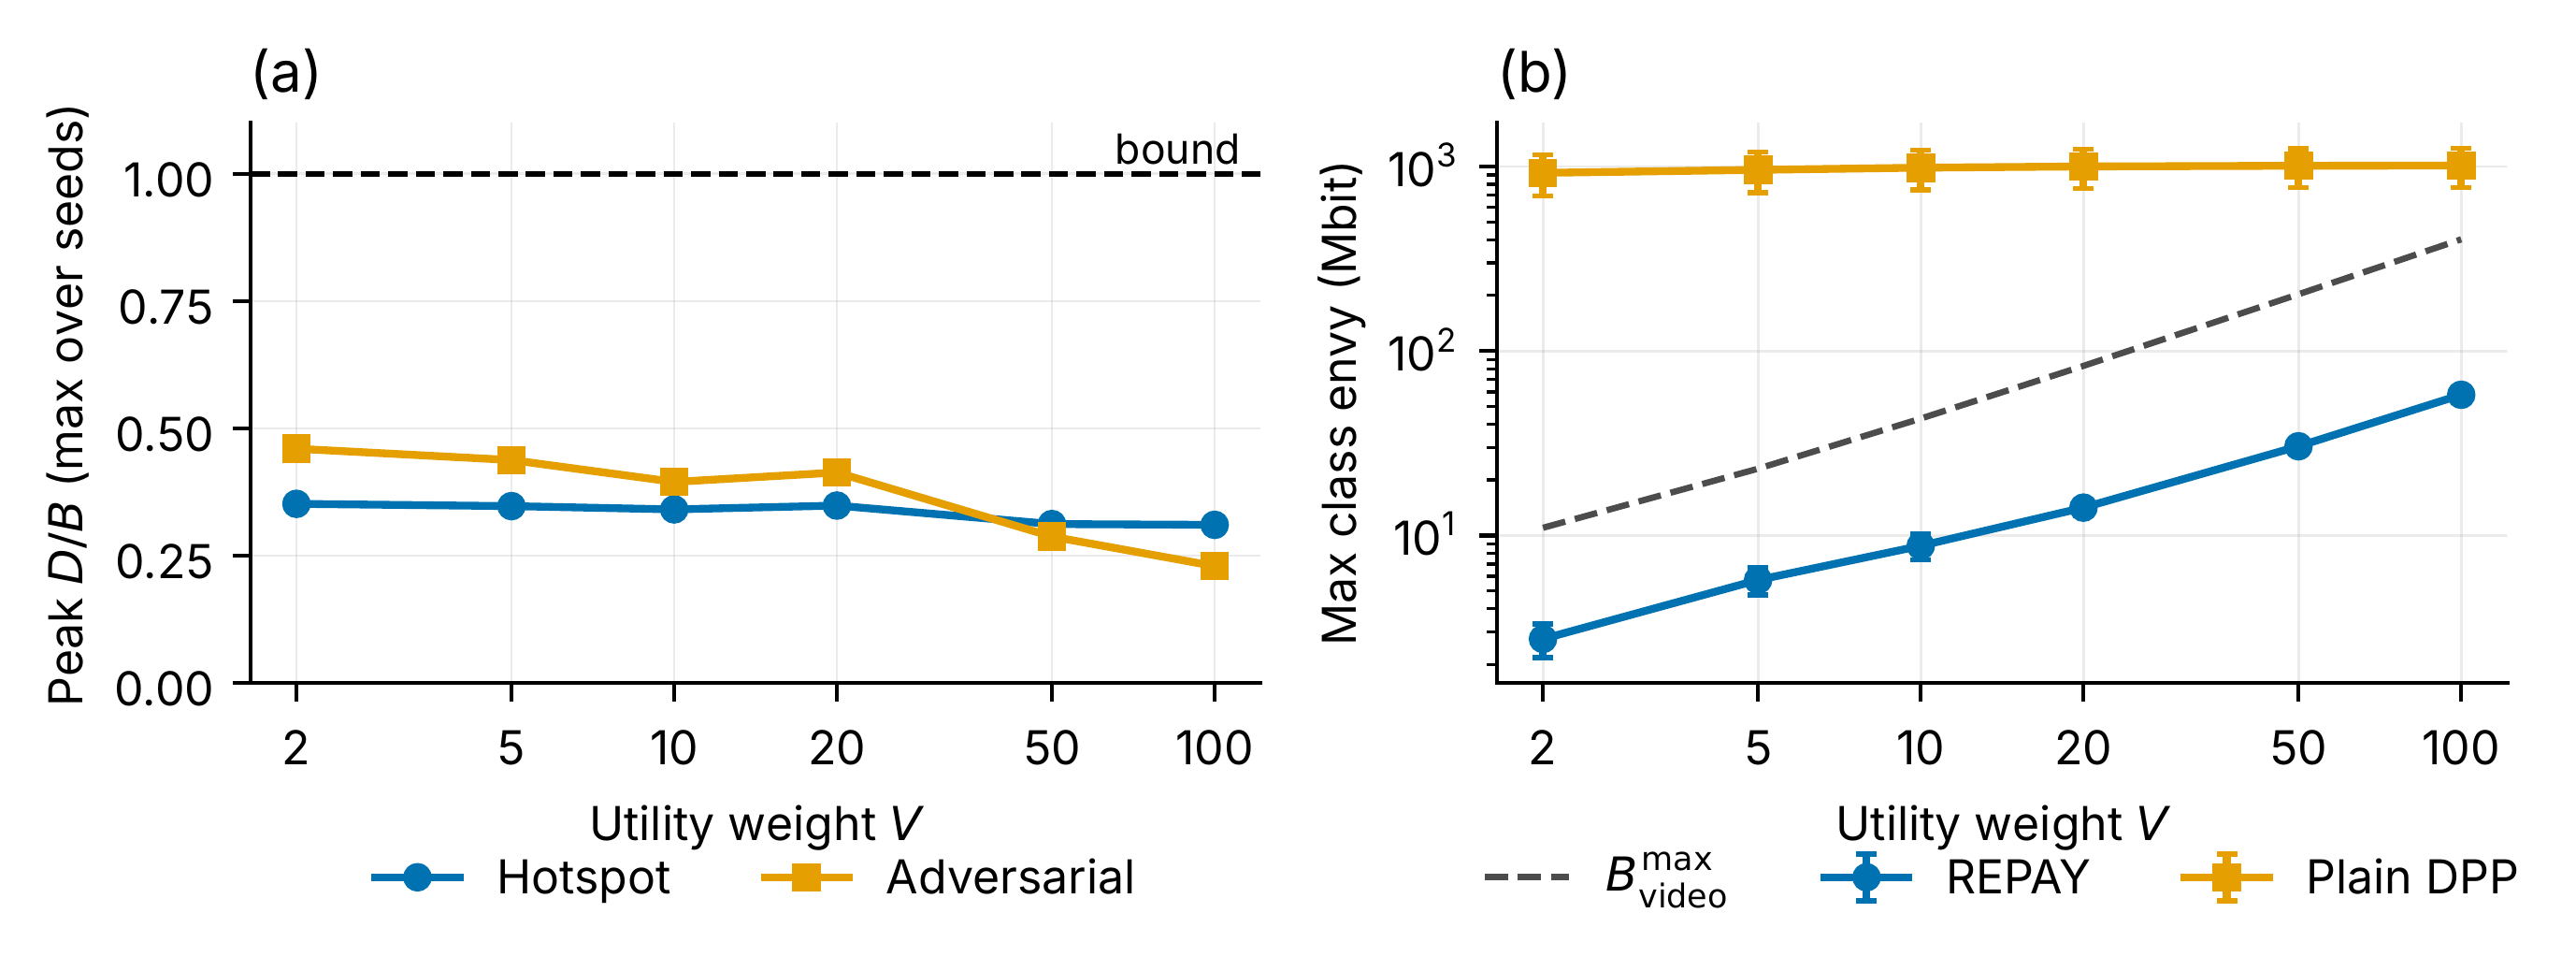
\includegraphics[width=\linewidth]{fig_bound.png}
\caption{(a) Largest deficit relative to the bound of Theorem~\ref{thm:bound} (maximum over seeds). (b) Maximum class envy of \repay{} and of the same rule without deficit queues; the dashed line is the largest video bound $\max_gB_{g,\mathrm{v}}$.}
\label{fig:bound}
\end{figure}

\subsection{Optimality gap}\label{sec:exp-opt}

To test Theorem~\ref{thm:opt} we fix a population (two tiers, three video flows, one gaming flow and five elastic devices with different demand caps), draw the capacity independently in each slot from $200$ equally likely values (sampled once from a mixture of lognormals with medians $30$, $12$ and $4$~Mbit/s), and compute the benchmark $U^*$ of \eqref{eq:bench} with a conic solver (with $\theta_P=0.5$ and $\phi=0.15$; three seeds for the simulation).
Both tier constraints turn out to be slack on this instance, so the gap is governed by the envy constraints, which enter the benchmark through the affine majorant; utility here is the operator's weighted objective.
Its value is $18.13$. Without the envy constraints the optimum is $18.22$, and with envy-freeness imposed in every slot instead of on average it drops to $17.78$: on this instance the whole value of time-shifting is $0.35$ and the cost of class-envy-freeness, once time-shifting is allowed, is $0.09$.
Figure~\ref{fig:optgap} shows the time-average fluid utility of \repay{} over $20\,000$ slots.
The gap to $U^*$ is $0.44$ at $V=5$, $0.091$ at $V=20$ and $0.030$ at $V=100$; the product of gap and $V$ lies between $1.82$ and $3.03$ for $V\ge5$, consistent with a gap of order $1/V$ (the constant $B_0$ of Theorem~\ref{thm:opt} is far larger than these values, so the bound itself is not tight), and already at $V=10$ \repay{} is above the slot-wise envy-free optimum, so it does exploit time-shifting.
Plain DPP reaches slightly more than $U^*$ because it ignores the envy constraints; class-blind PF obtains $17.52$.
The largest deficit in these runs is $0.21$ of its bound.

\begin{figure}[t]
\centering
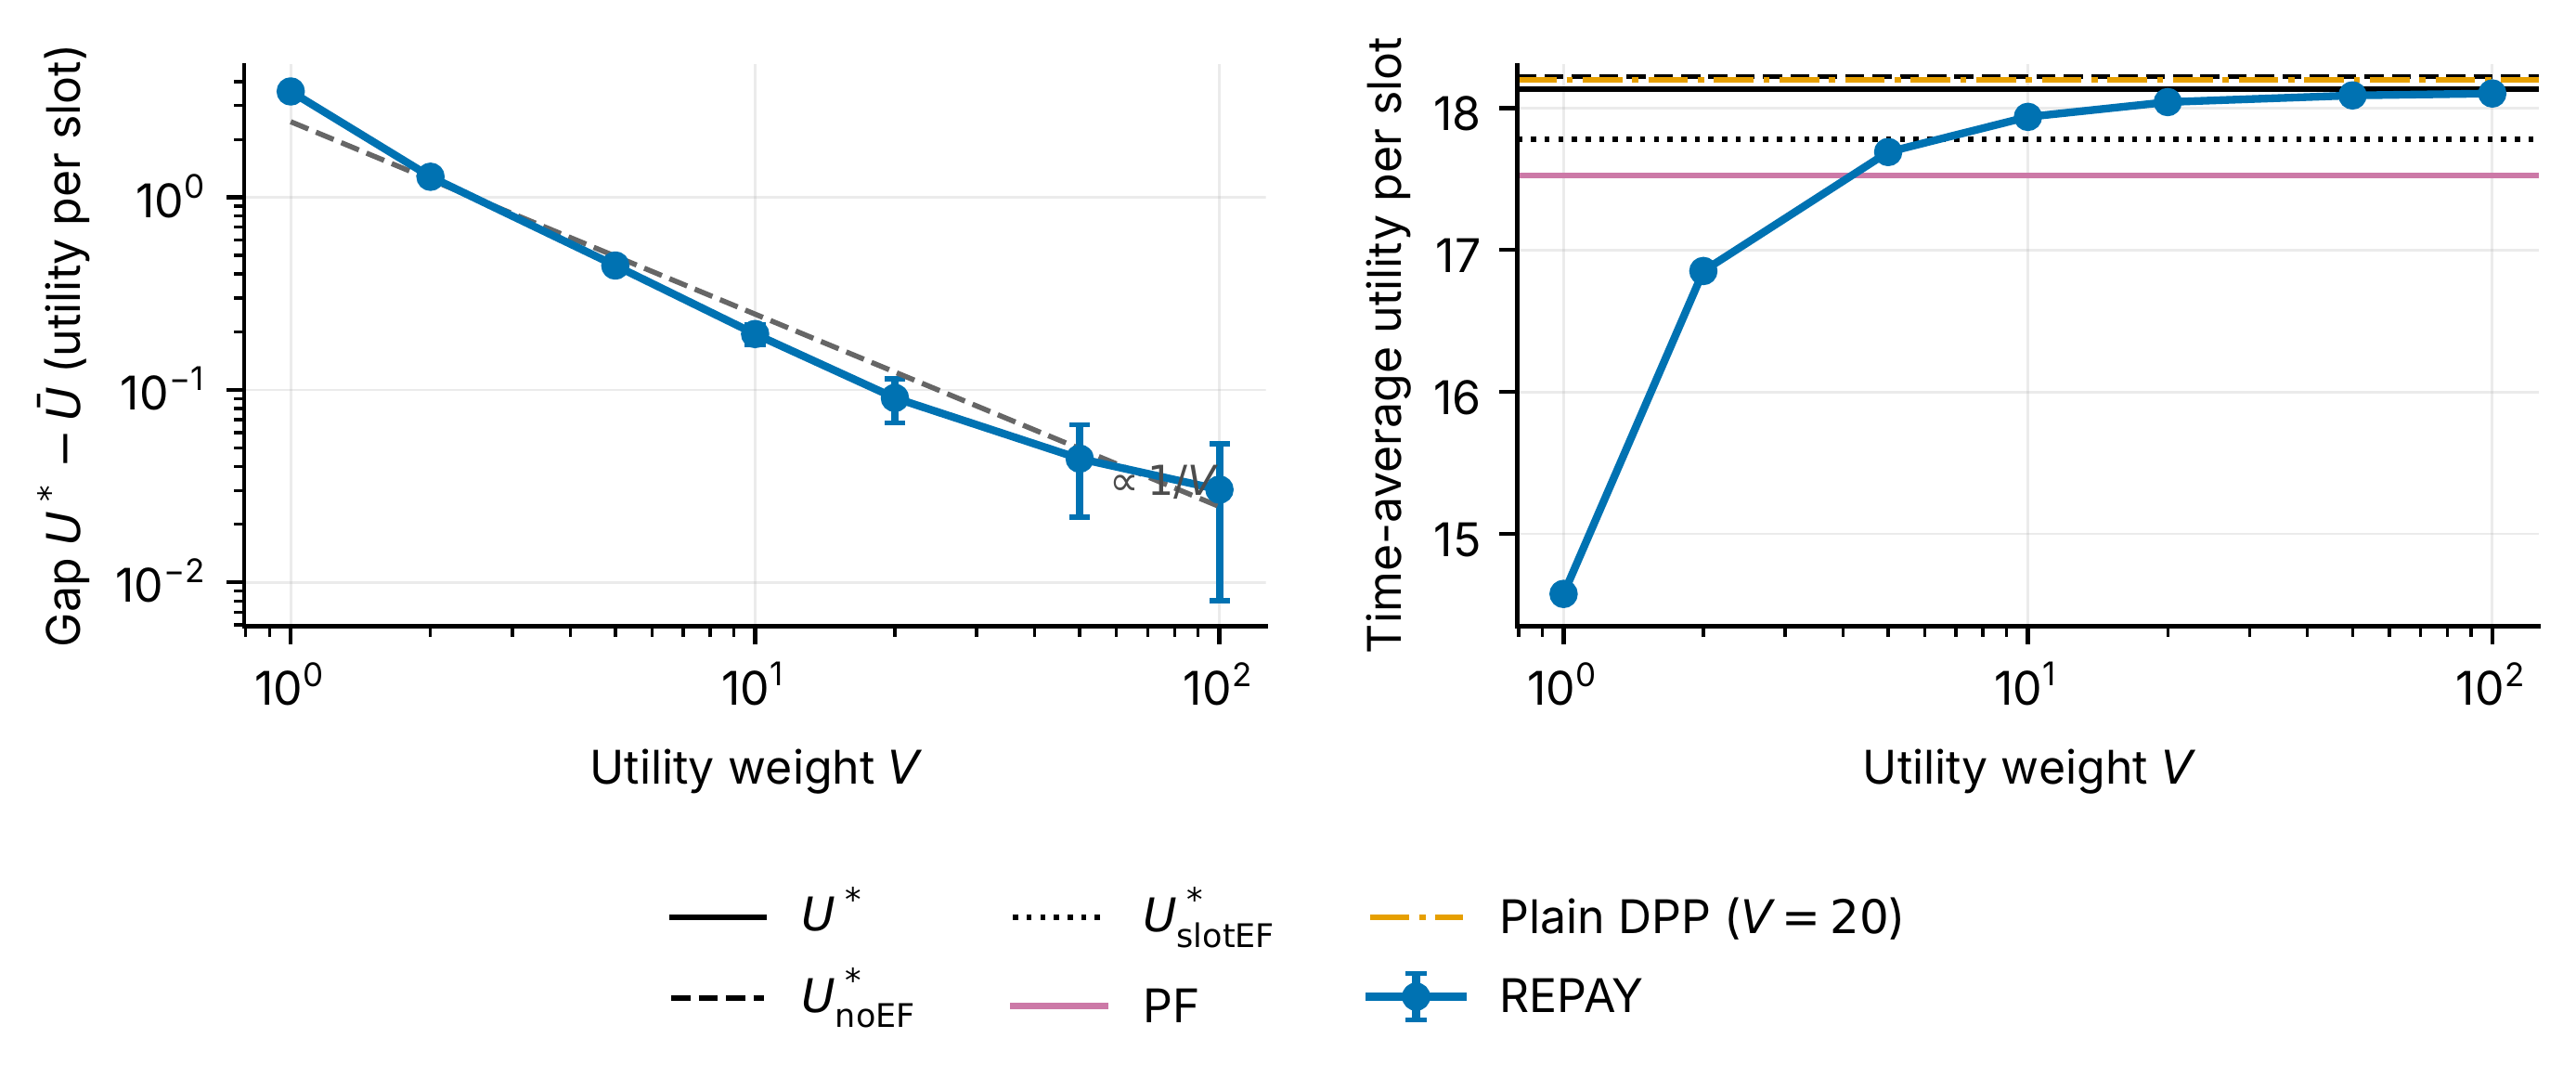
\includegraphics[width=\linewidth]{fig_optgap.png}
\caption{Optimality gap on a fixed population with i.i.d.\ capacity. Left: gap to the benchmark $U^*$ against $V$. Right: average utility against the three benchmark values.}
\label{fig:optgap}
\end{figure}

\subsection{Comparison with truthful devices}\label{sec:exp-compare}

Table~\ref{tab:compare} and Figure~\ref{fig:compare} compare all rules on the hotspot scenario when every device declares its true class ($10$ seeds, $6000$ slots).
The rules fall into three groups.
\textsc{WFQ} and \textsc{Priority} serve nearly all RT slots, but they do so by taking capacity from elastic devices for good: the elastic rate falls from about $1.75$ to $1.26$--$1.27$~Mbit/s and class envy reaches $2000$ to $2200$~Mbit; plain DPP serves $99.9\%$ of RT slots with an elastic rate of $1.52$~Mbit/s and class envy of $1070$~Mbit.
\textsc{PF} and \textsc{Credit} are fair to elastic devices and leave RT flows unprotected ($82$--$83\%$ of RT slots, $76$--$80\%$ for video).
\repay{} serves $95.0\%$ of RT slots while giving elastic devices almost what \textsc{PF} gives them ($1.74$ against $1.78$~Mbit/s) and keeping class envy at $15$~Mbit.
It closes $72\%$ of the gap in RT success between \textsc{PF} and \textsc{Priority} at a $2.3\%$ lower elastic rate and with a higher utility than \textsc{PF}.
The intervals in the table overlap because the traces differ more than the rules do; the paired differences between \repay{} and \textsc{PF} over the ten traces are $+13.1\pm1.3$ points of RT success, $+3.9\pm0.3$ in utility and $-0.040\pm0.004$~Mbit/s in elastic rate, each with the same sign on every trace.
Plain DPP, which differs from \repay{} only by the deficit queues, serves $4.9\pm1.3$ points more RT slots and has a utility higher by $2.2\pm0.3$, with an elastic rate lower by $0.23$~Mbit/s ($13\%$): this is the price of bounded envy when everyone is truthful.
The utility figures add real-time and elastic utilities on the scales of Section~\ref{sec:model}, so their ranking depends on that exchange rate; RT success and elastic rate do not.
The gain is in the free tier, where $92\%$ of RT slots are served against $70\%$ under \textsc{PF}; the paid tiers are served in more than $99\%$ of slots by every rule except \textsc{Credit} ($95\%$ for premium and $84\%$ for PAYG). These per-tier figures are computed from the result files and are not in the table.
When all devices are truthful, \textsc{Priority}, plain DPP and \textsc{WFQ} have the highest utility ($74.8$, $74.7$ and $73.9$ against $72.6$ for \repay{}); their defects are envy and, as Section~\ref{sec:exp-strategic} shows, incentives.
\textsc{Repay-WC} coincides with \repay{} in every run, so its recycling condition (spare capacity while every elastic device is at its cap) has no effect in any run and the variant is not exercised by our experiments. \textsc{Repay-E} differs by about $0.01$ in utility and $0.05$ points in video success: the entrant offer matters when a tier has no RT flow, which is rare with $75$ devices.
Dropping the debt price (No-debt) raises RT success by $2.6\pm0.5$ points and class envy from $15$ to $25$~Mbit, at an elastic rate lower by $0.025$~Mbit/s.

In the home scenario capacity is ample most of the time and all rules serve $97\%$ of RT slots or more (Table~\ref{tab:compare-home}); the differences are again in class envy, $10$~Mbit for \repay{} against $165$ for plain DPP and $460$ for \textsc{WFQ} and \textsc{Priority}, which coincide on this scenario because RT flows never have to be rationed.

\begin{table}[t]
\centering
\caption{Hotspot scenario, truthful devices (mean over 10 seeds, $\pm$ half-width of the 95\% confidence interval). Premium and PAYG ratios are served volume over committed demand and the free-floor ratio is served volume over the floor; the targets are $0.8$, $0.6$ and $1$. Utility is the unweighted sum of true utilities.}
\label{tab:compare}
\resizebox{\linewidth}{!}{\begin{tabular}{lrrrrrrrrrr}
\toprule
Mechanism & Utility & RT success (\%) & Video success (\%) & Elastic rate (Mbit/s) & Jain index & Premium ratio & PAYG ratio & Free-floor ratio & Max class envy (Mbit) & 95th-pct.\ device envy (Mbit) \\
\midrule
REPAY & 72.6 $\pm$ 2.4 & 95.0 $\pm$ 1.3 & 93.1 $\pm$ 1.8 & 1.74 & 0.791 & 1.32 & 1.29 & 2.90 & 14.6 $\pm$ 1.5 & 11.4 \\
REPAY-WC & 72.6 $\pm$ 2.4 & 95.0 $\pm$ 1.3 & 93.1 $\pm$ 1.8 & 1.74 & 0.791 & 1.32 & 1.29 & 2.90 & 14.6 $\pm$ 1.5 & 11.4 \\
REPAY-E & 72.6 $\pm$ 2.4 & 95.0 $\pm$ 1.3 & 93.0 $\pm$ 1.8 & 1.74 & 0.791 & 1.32 & 1.30 & 2.90 & 14.6 $\pm$ 1.5 & 11.4 \\
No-debt & 73.6 $\pm$ 2.4 & 97.6 $\pm$ 1.0 & 96.7 $\pm$ 1.4 & 1.72 & 0.787 & 1.22 & 1.24 & 3.15 & 25.1 $\pm$ 0.5 & 23.4 \\
Plain DPP & 74.7 $\pm$ 2.3 & 99.9 $\pm$ 0.1 & 99.9 $\pm$ 0.2 & 1.52 & 0.707 & 1.35 & 1.30 & 2.85 & 1072.1 $\pm$ 163.0 & 370.6 \\
PF & 68.7 $\pm$ 2.6 & 81.9 $\pm$ 2.2 & 79.8 $\pm$ 2.3 & 1.78 & 0.783 & 1.44 & 1.36 & 2.62 & 0.0 $\pm$ 0.0 & 0.0 \\
WFQ & 73.9 $\pm$ 2.2 & 98.7 $\pm$ 0.6 & 98.2 $\pm$ 0.8 & 1.27 & 0.630 & 1.22 & 1.25 & 3.14 & 1980.6 $\pm$ 290.2 & 708.9 \\
Priority & 74.8 $\pm$ 2.3 & 100.0 $\pm$ 0.0 & 100.0 $\pm$ 0.0 & 1.26 & 0.625 & 1.15 & 1.22 & 3.31 & 2211.7 $\pm$ 328.7 & 763.8 \\
Credit & 64.4 $\pm$ 2.5 & 82.6 $\pm$ 2.5 & 75.7 $\pm$ 3.1 & 1.87 & 0.800 & 1.21 & 1.24 & 3.17 & 127.4 $\pm$ 28.4 & 35.6 \\
\bottomrule
\end{tabular}}
\end{table}

\begin{table}[t]
\centering
\caption{Home scenario, truthful devices (mean over 10 seeds).}
\label{tab:compare-home}
\resizebox{0.85\linewidth}{!}{\begin{tabular}{lrrrrrrrr}
\toprule
Mechanism & Utility & RT success (\%) & Video success (\%) & Elastic rate (Mbit/s) & Jain index & Premium ratio & Max class envy (Mbit) & 95th-pct.\ device envy (Mbit) \\
\midrule
REPAY & 7.9 $\pm$ 0.3 & 100.0 $\pm$ 0.0 & 100.0 $\pm$ 0.0 & 3.19 & 0.998 & 1.47 & 10.3 $\pm$ 2.2 & 10.3 \\
REPAY-WC & 7.9 $\pm$ 0.3 & 100.0 $\pm$ 0.0 & 100.0 $\pm$ 0.0 & 3.19 & 0.998 & 1.47 & 10.3 $\pm$ 2.2 & 10.3 \\
REPAY-E & 7.8 $\pm$ 0.3 & 100.0 $\pm$ 0.0 & 100.0 $\pm$ 0.0 & 3.19 & 0.998 & 1.47 & 10.2 $\pm$ 2.2 & 10.1 \\
No-debt & 7.9 $\pm$ 0.3 & 100.0 $\pm$ 0.0 & 100.0 $\pm$ 0.0 & 3.18 & 0.998 & 1.47 & 24.2 $\pm$ 2.5 & 24.2 \\
Plain DPP & 7.9 $\pm$ 0.3 & 100.0 $\pm$ 0.0 & 100.0 $\pm$ 0.0 & 3.13 & 0.997 & 1.47 & 164.5 $\pm$ 37.3 & 163.1 \\
PF & 7.8 $\pm$ 0.3 & 99.3 $\pm$ 0.5 & 99.1 $\pm$ 0.6 & 3.20 & 0.998 & 1.47 & 0.0 $\pm$ 0.0 & 0.0 \\
WFQ & 7.8 $\pm$ 0.3 & 100.0 $\pm$ 0.0 & 100.0 $\pm$ 0.0 & 3.05 & 0.997 & 1.47 & 459.4 $\pm$ 143.6 & 447.2 \\
Priority & 7.8 $\pm$ 0.3 & 100.0 $\pm$ 0.0 & 100.0 $\pm$ 0.0 & 3.05 & 0.997 & 1.47 & 459.4 $\pm$ 143.6 & 447.2 \\
Credit & 7.6 $\pm$ 0.3 & 97.0 $\pm$ 2.4 & 96.1 $\pm$ 2.6 & 3.18 & 0.998 & 1.47 & 120.1 $\pm$ 37.9 & 115.7 \\
\bottomrule
\end{tabular}}
\end{table}

\begin{figure}[t]
\centering
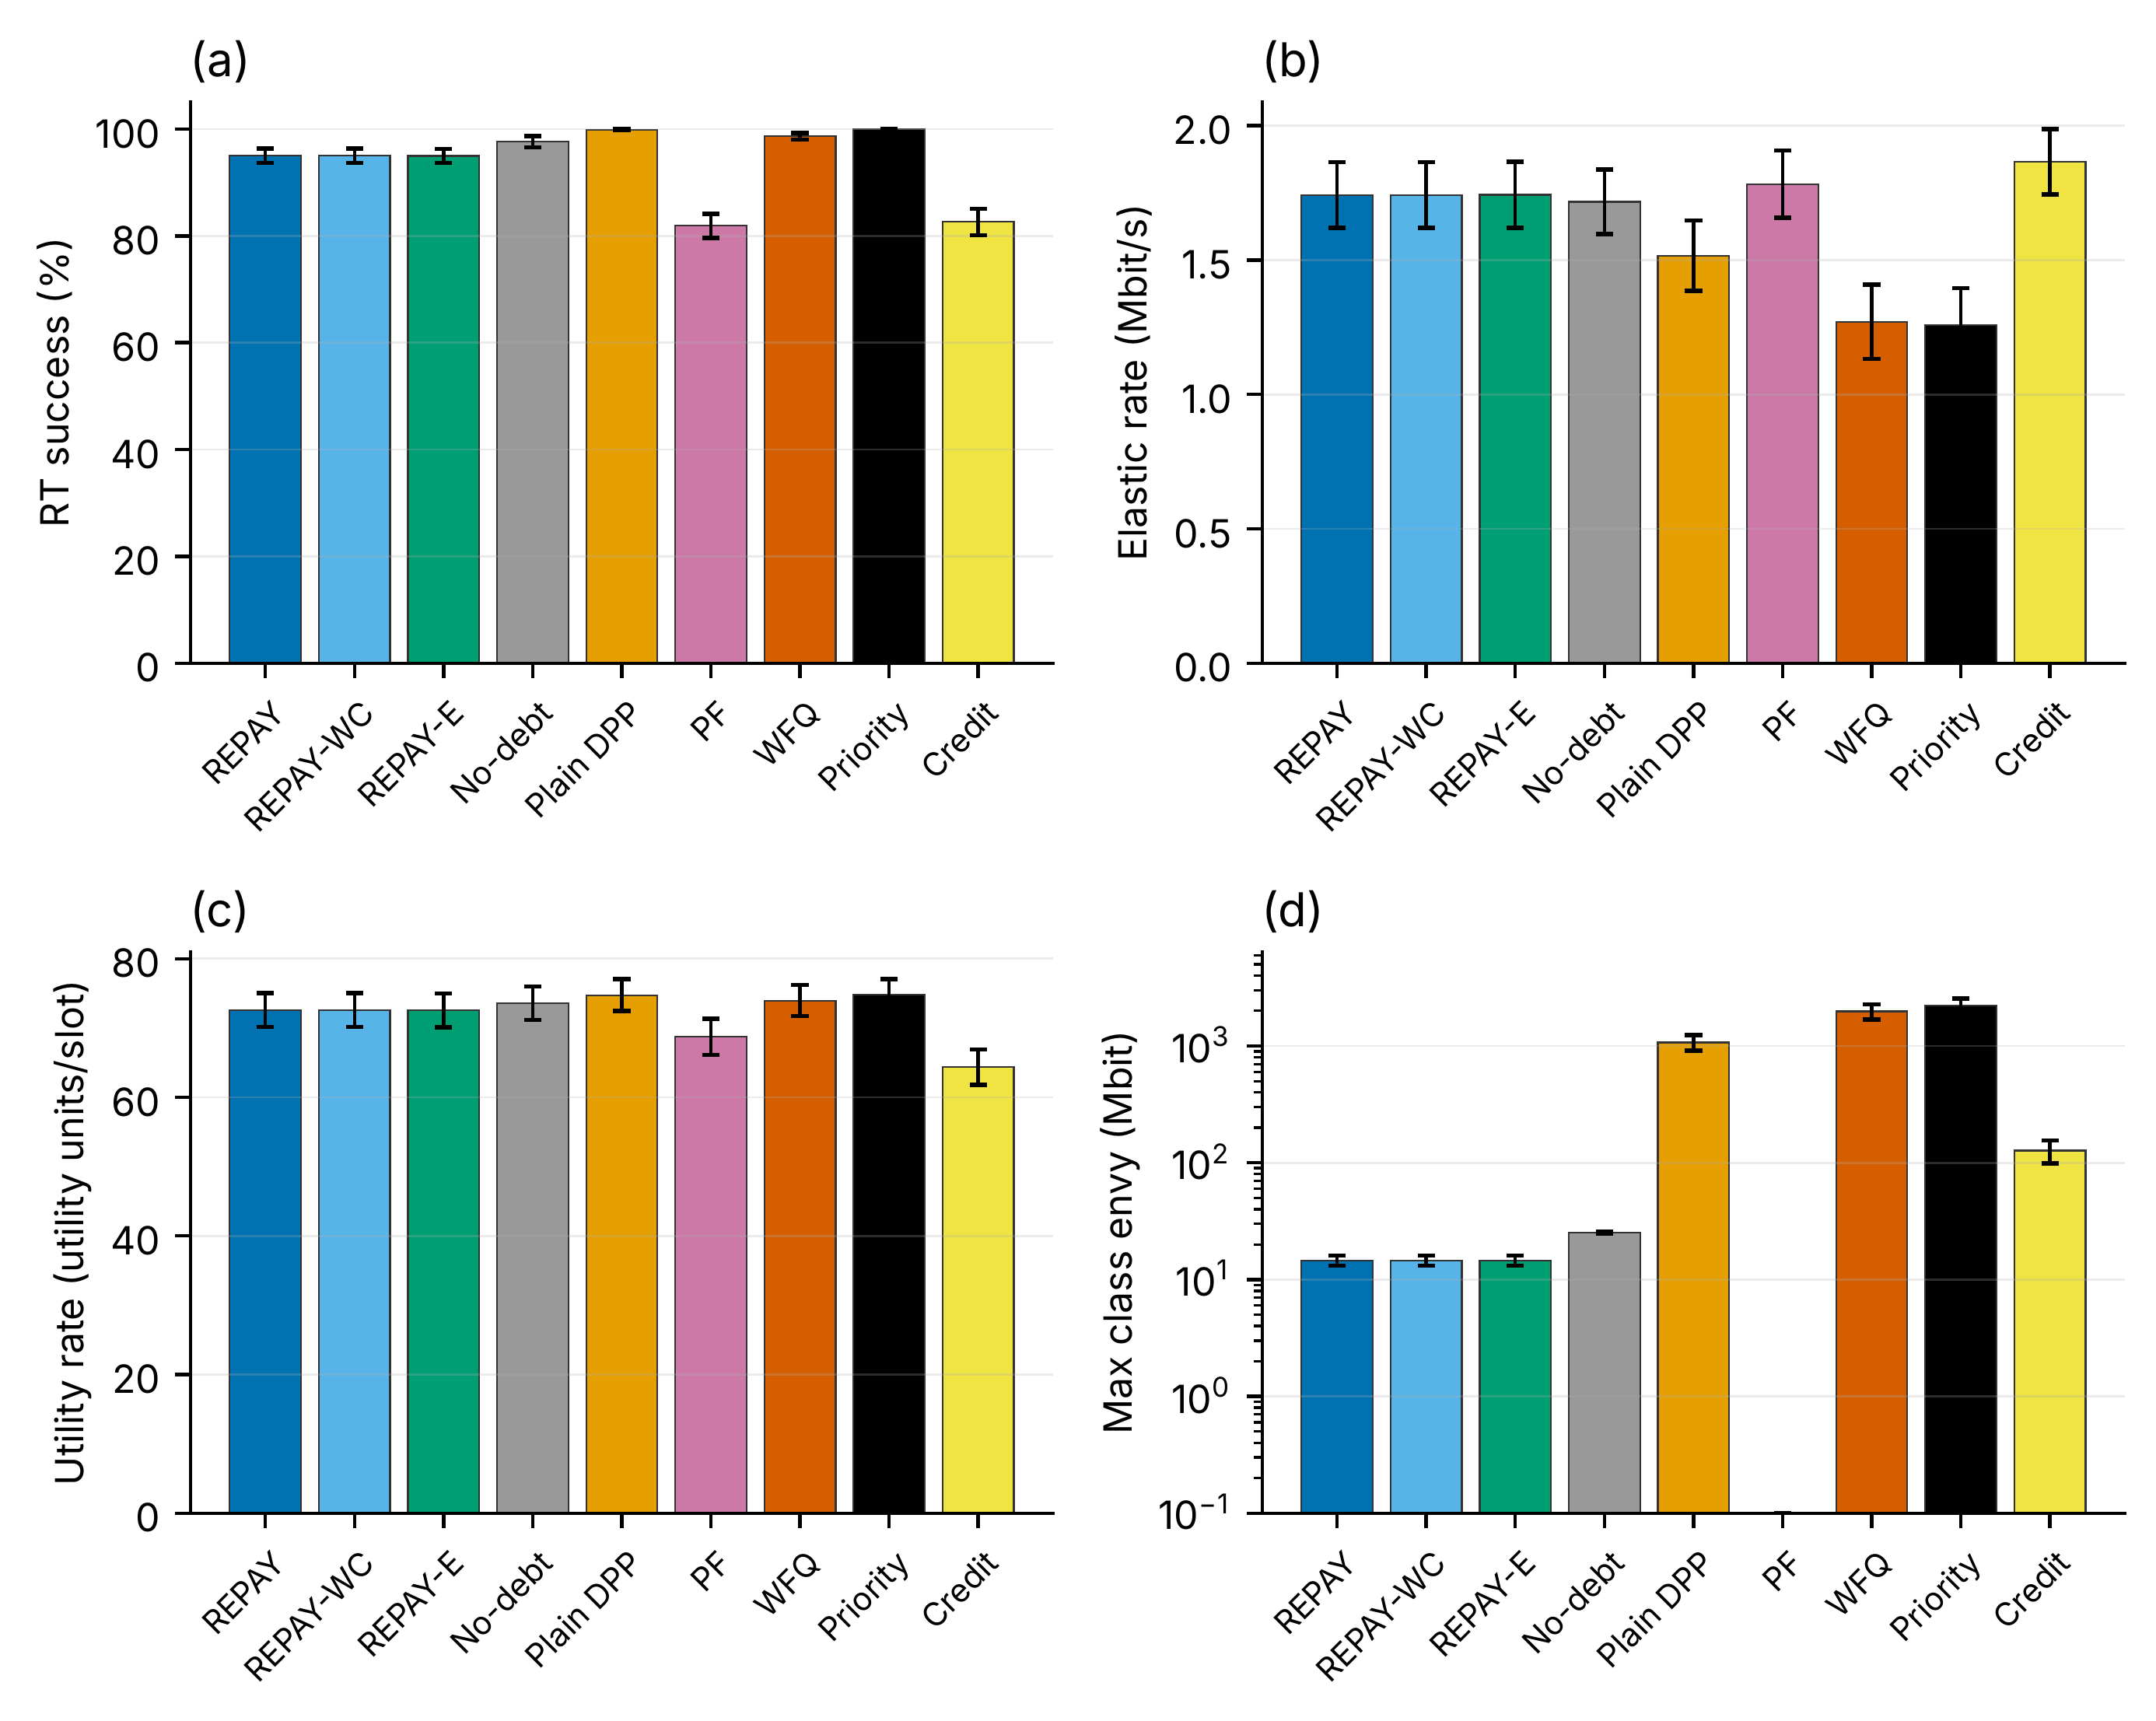
\includegraphics[width=0.9\linewidth]{fig_compare.png}
\caption{Hotspot scenario, truthful devices: (a) RT success, (b) elastic rate, (c) utility, (d) maximum class envy (logarithmic scale; \textsc{PF} has none).}
\label{fig:compare}
\end{figure}

\paragraph{Trade-off curves and a capped priority.}
Each rule has a parameter that moves it between protecting RT flows and serving elastic devices, and a single setting can flatter or penalise it.
Figure~\ref{fig:frontier} therefore sweeps $V$ for \repay{} and plain DPP and the RT weight multiplier for \textsc{WFQ}, on five traces.
We also add a baseline that a practitioner would try first, \emph{capped priority}: strict priority in which declared RT flows may use at most a fraction $q$ of the capacity of the slot, so that the reward for declaring RT is limited by construction.
\repay{} lies to the right of plain DPP and \textsc{WFQ} at every level of RT success, that is, it protects the same share of RT slots while leaving more to elastic devices.
Capped priority, however, does better than \repay{} on this pair of metrics around $q=0.3$: there it serves $93.2\%$ of RT slots with an elastic rate of $1.80$~Mbit/s, against $92.3\%$ and $1.67$ for \repay{} at $V=10$ and $94.4\%$ and $1.66$ at $V=20$, because it holds admitted calls close to their minimum rate; its utility is lower ($70.1$ against $71.9$ for \repay{} at $V=20$). At $q=0.5$ it is below the curve of \repay{} ($99.5\%$ at $1.46$~Mbit/s, against $99.3\%$ at $1.63$ for \repay{} at $V=100$).
Table~\ref{tab:cap} shows what it gives up.
Its class envy is $390$~Mbit at $q=0.3$, about $28$ times that of \repay{} at $V=20$, and grows quickly with $q$; and its resistance to misreporting depends on the cap being tight for the traffic mix at hand: with $q=0.2$ or $0.3$ a misreporting device loses on average and $2\%$ or $25\%$ of the devices gain, fewer than under \repay{} on the same $60$ devices ($58\%$, median change $+1.5\%$); with $q=0.5$ the median device gains $69\%$.
When the share of real-time devices falls from $35\%$ to $10\%$, the same cap $q=0.3$ no longer binds and the median misreporting device gains $113\%$, against $-0.9\%$ under \repay{} (Section~\ref{sec:exp-mix}); the right cap thus depends on the share of real-time traffic, which the operator does not know and which changes during the day, whereas $V$ sets the envy bound whatever the mix.
We read this as follows. If an operator only needs calls to survive short shortages, knows its traffic mix and can tune a cap, capped priority is a simple and effective answer, and the case for \repay{} rests on what it guarantees to each elastic device, not on average performance.

\begin{figure}[t]
\centering
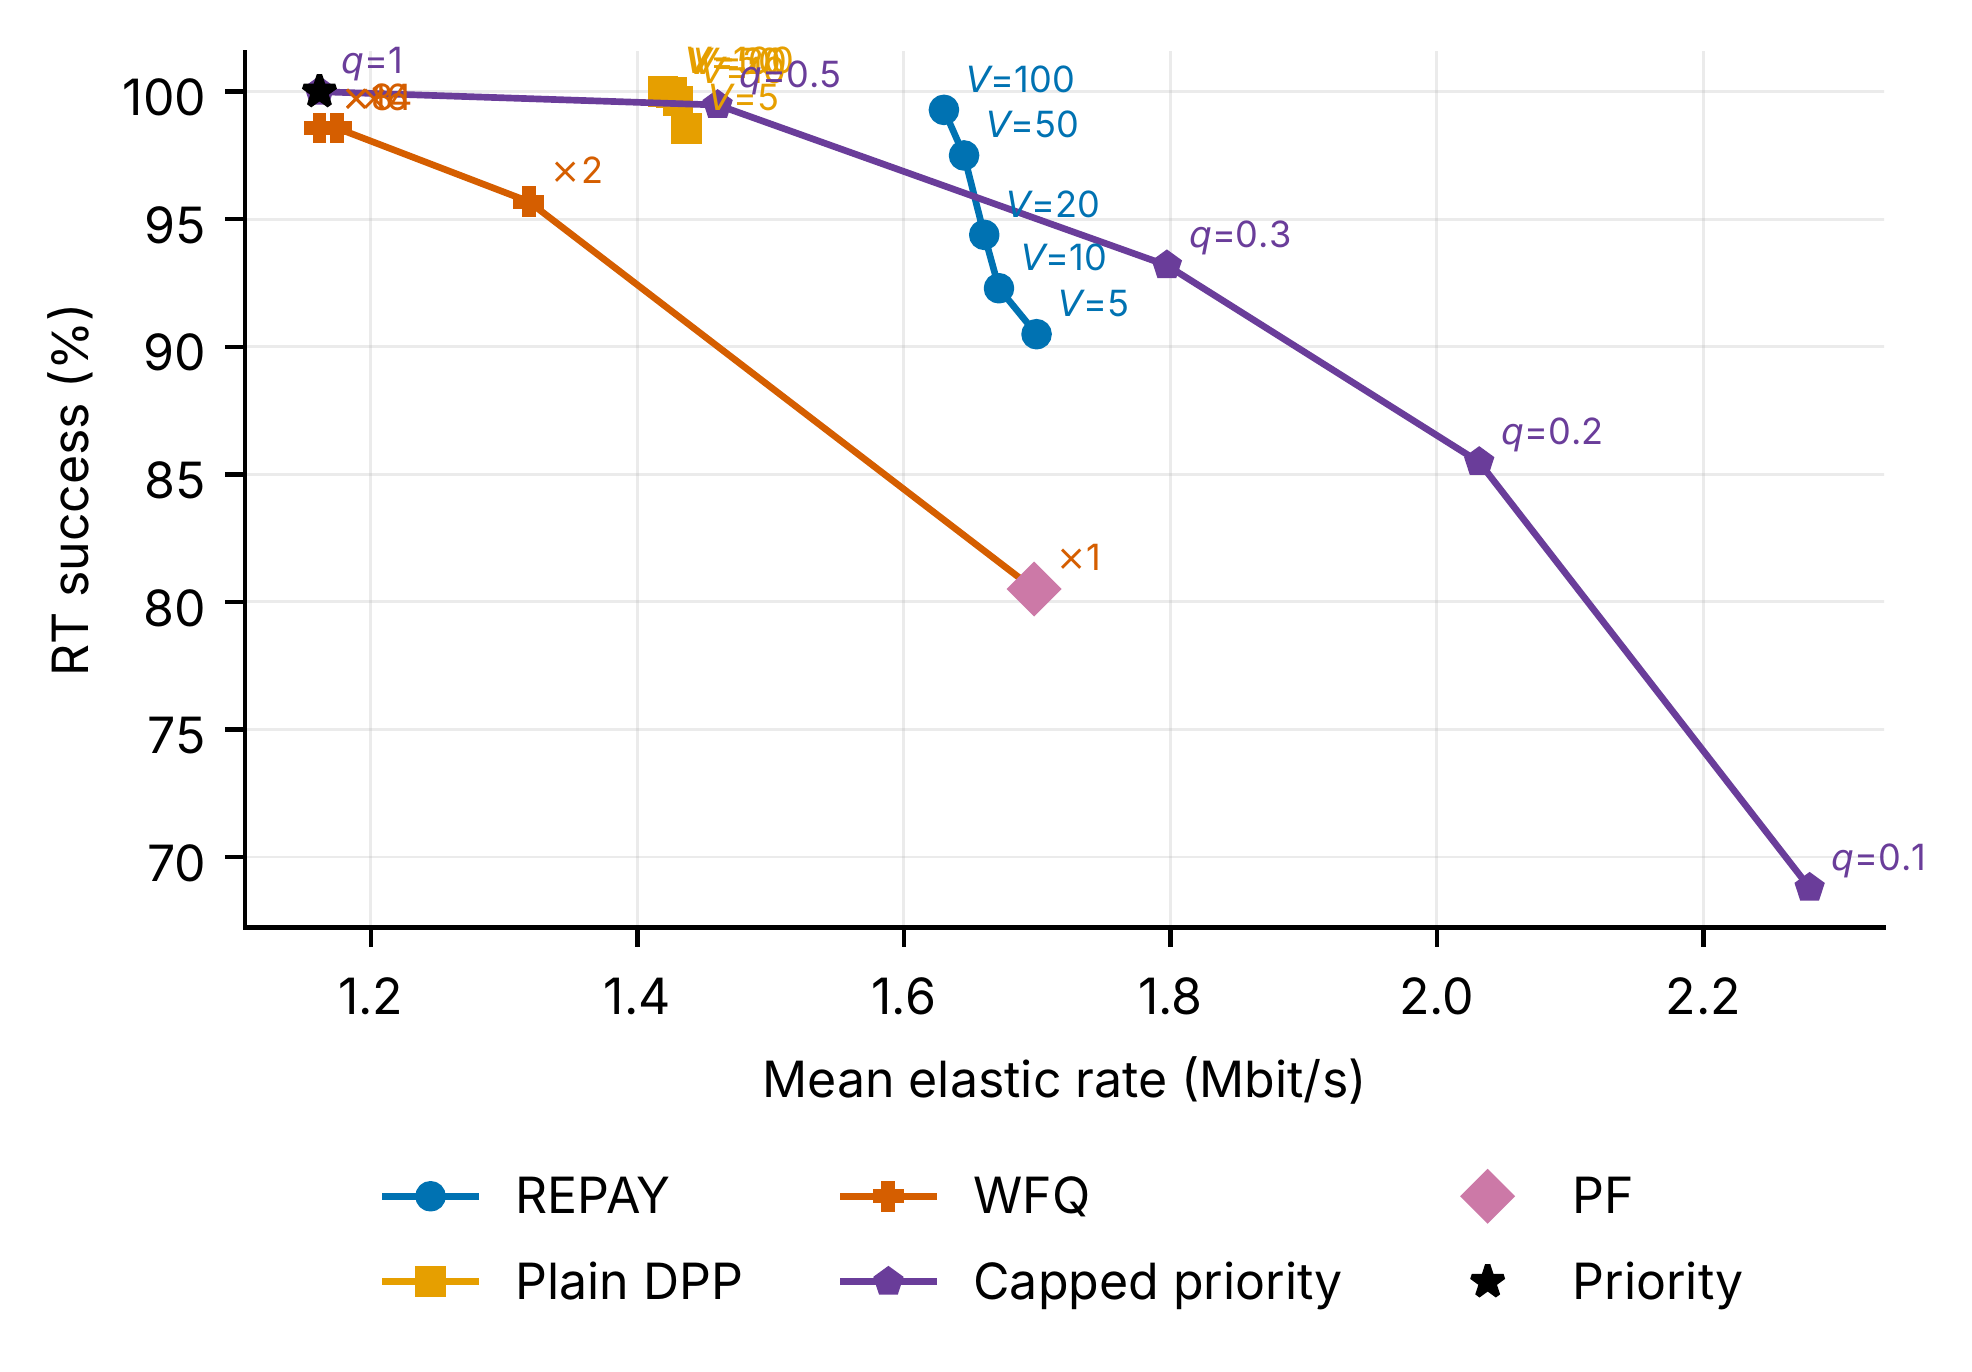
\includegraphics[width=0.7\linewidth]{fig_frontier.png}
\caption{RT success against elastic rate when the parameter of each rule is varied (hotspot, truthful devices, mean over five traces).}
\label{fig:frontier}
\end{figure}

\begin{table}[t]
\centering
\caption{Capped priority: RT flows may use at most a fraction $q$ of capacity. Left columns: truthful devices, five traces. Right columns: one elastic device declares video ($60$ devices on two traces, as in Section~\ref{sec:exp-strategic}).}
\label{tab:cap}
\resizebox{\linewidth}{!}{\begin{tabular}{rrrrrrr}
\toprule
$q$ & RT success (\%) & Elastic rate (Mbit/s) & Max class envy (Mbit) & Median rel.\ gain of misreport (\%) & Pooled volume gain (\%) & Devices gaining (\%) \\
\midrule
0.1 & 68.8 $\pm$ 1.0 & 2.28 $\pm$ 0.14 & 1.57 $\pm$ 2.65 & -- & -- & -- \\
0.2 & 85.5 $\pm$ 1.0 & 2.03 $\pm$ 0.12 & 67.97 $\pm$ 49.92 & -55.33 & -60.40 & 1.7 \\
0.3 & 93.2 $\pm$ 1.2 & 1.80 $\pm$ 0.11 & 390.66 $\pm$ 169.75 & -20.27 & -33.03 & 25.0 \\
0.5 & 99.5 $\pm$ 0.4 & 1.46 $\pm$ 0.08 & 1296.82 $\pm$ 216.89 & 68.74 & 27.02 & 66.7 \\
1 & 100.0 $\pm$ 0.0 & 1.16 $\pm$ 0.06 & 2065.24 $\pm$ 593.74 & -- & -- & -- \\
\bottomrule
\end{tabular}}
\end{table}

\paragraph{Call continuity.}
RT success counts slots, and a call that is cut for one second every few seconds is worse than the count suggests.
Table~\ref{tab:continuity} reports the interruptions of genuine video calls on five traces.
Under \repay{} a call is below its minimum rate in $7.6\%$ of its slots; outages last $2.8$~s on average and $8.2$~s at the 95th percentile, there are $2.8$ of them per $100$~s of call, and $54\%$ of the calls are never interrupted.
Plain DPP almost never interrupts a call ($0.06\%$ of slots), \textsc{WFQ} and \textsc{Priority} rarely or never, and \textsc{PF} is worse in the way that matters most: its outages are rarer ($1.3$ per $100$~s) but last $17$~s on average, and they cover $22\%$ of the slots of a call.
The rotation inside a partially admitted group is not the cause of the interruptions. Two variants of the admission order (rows \textsc{Repay}-sticky and \textsc{Repay}-block of the table), one that keeps incumbents admitted and one that rotates only every ten slots, give the same outage share and an interruption rate and mean outage length within $0.04$ of those of \repay{} (the 95th percentile differs by at most $0.6$~s), because a whole tier--class group is usually admitted or refused together.
The interruptions come from the allocation itself, which stops admitting a group when its debt price is high, and reducing them would require a cost of interruption in the objective, which our model does not have.

\begin{table}[t]
\centering
\caption{Interruptions of genuine video calls (hotspot, truthful devices, five traces). An outage is a maximal run of slots below $\rmin_{\mathrm{v}}$.}
\label{tab:continuity}
\resizebox{\linewidth}{!}{\begin{tabular}{lrrrrrr}
\toprule
Mechanism & Outage slots (\%) & Interruptions per 100 s & Mean outage length (s) & 95th pct.\ outage length (s) & Outage in runs $\geq 5$ s (\%) & Calls never interrupted (\%) \\
\midrule
REPAY & 7.61 & 2.76 & 2.79 & 8.2 & 46.6 & 53.7 \\
REPAY-sticky & 7.61 & 2.72 & 2.83 & 8.6 & 47.2 & 53.8 \\
REPAY-block & 7.61 & 2.73 & 2.82 & 8.8 & 46.8 & 53.7 \\
Plain DPP & 0.06 & 0.05 & 1.06 & 1.4 & 0.0 & 93.6 \\
PF & 21.71 & 1.33 & 17.27 & 65.9 & 94.7 & 42.1 \\
WFQ & 1.93 & 1.13 & 1.57 & 3.6 & 12.8 & 69.5 \\
Priority & 0.00 & 0.00 & -- & -- & -- & 100.0 \\
\bottomrule
\end{tabular}}
\end{table}

\paragraph{Capacity variability.}
Figure~\ref{fig:variability} varies the spread of the capacity states while holding the mean at $90$~Mbit/s.
With constant capacity every rule serves at least $99\%$ of the RT slots.
As shortages become deeper, \textsc{PF} and \textsc{Credit} lose RT slots first; \repay{} stays within six points of plain DPP at every spread ($5.6$ points at the default spread), and at the most severe spread it serves $82.5\%$ of RT slots against $85.7\%$ for plain DPP, $78.7\%$ for \textsc{WFQ} and $70.5\%$ for \textsc{PF}.
Only \textsc{Priority} remains above $90\%$ there, with class envy above $1500$~Mbit.
In that regime the fair share stays below $\rmin_{\mathrm{v}}$ for long periods and bounded envy forces rationing, as described at the end of Section~\ref{sec:baselines-theory}.

\begin{figure}[t]
\centering
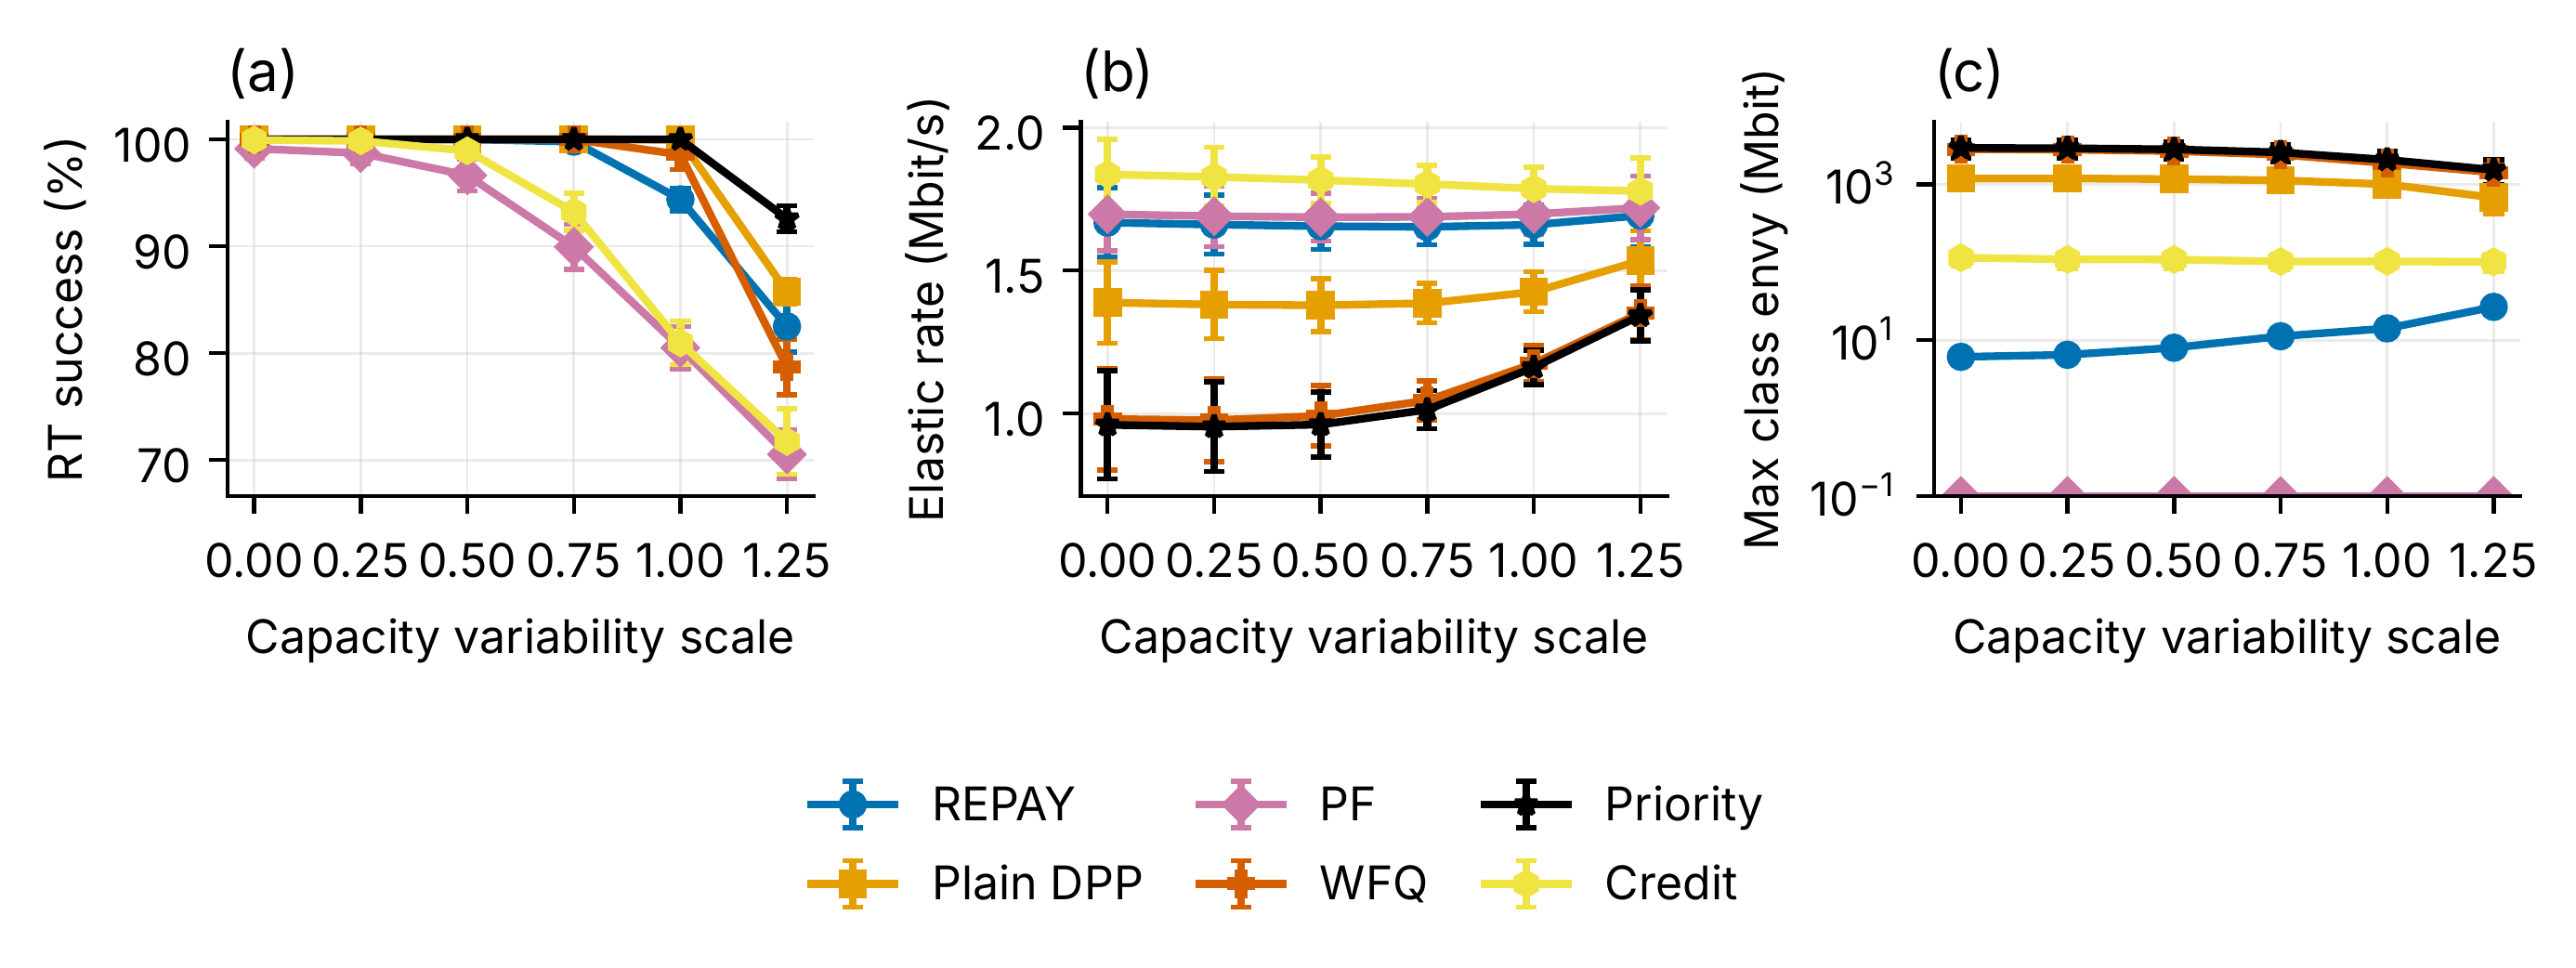
\includegraphics[width=\linewidth]{fig_variability.png}
\caption{Effect of capacity variability (scale $0$: constant capacity; scale $1$: the default hotspot scenario) at equal mean capacity.}
\label{fig:variability}
\end{figure}

\subsection{Strategic devices}\label{sec:exp-strategic}

\paragraph{Unilateral deviations.}
We take $30$ elastic devices per trace (six traces of $3000$ slots, devices present for at least $60$ slots, $180$ devices in all) and, for each of them and each rule, re-run the whole simulation with that device declaring video for its entire stay.
This measures the exact gain, including the effect of the deviation on prices and offers that the price-taking analysis ignores.
Table~\ref{tab:deviation} and Figure~\ref{fig:deviation} report the change in the volume the device receives; since relative gains are skewed by devices that receive little when truthful, we give the median and the mean of the per-device relative gain and the pooled change in volume, with confidence intervals from a bootstrap over traces.
Under \textsc{Priority} and \textsc{WFQ} misreporting pays for more than nine devices in ten: the median device gains $170\%$ and $154\%$, and the pooled volume doubles ($+105\%$ and $+100\%$).
Under plain DPP the median gain is $77\%$ and the pooled gain $35\%$.
Under \repay{} the median change is $+1.3\%$, with a confidence interval of $[0.8,1.5]$, the mean change is $-0.1\%$, and the pooled volume falls by $10\%$.
The deviation is not harmless for everyone: $63\%$ of the devices gain something, but the gains are small (the 95th percentile is $0.09$~Mbit/s and the largest gain over a whole stay is $47$~Mbit, $4\%$ of that device's volume), and no device gains more than its bound $B_{g,\mathrm{v}}$, although the largest gain reaches $0.75$ of it, so the externality term left open after Theorem~\ref{thm:static} is not negligible here.
The picture differs by tier. Free devices, whose fair share is often below the video rate, gain a median of $2.0\%$ and $83\%$ of them gain; PAYG devices gain a median of $2.3\%$ ($67\%$ gain), although their pooled volume falls by $17\%$; premium devices lose a median of $13\%$ and only $5\%$ of them gain.
Part of the losses comes from the experiment itself: every sampled device has a link rate above $3$~Mbit/s, so declaring video caps it at $\rmax_{\mathrm{v}}$ whenever capacity is plentiful.
This is why the pooled volume also falls under \textsc{PF} and \textsc{Credit}, which ignore the declaration altogether, and the comparison that matters is between \repay{} and the rules that do use the class.

\paragraph{Short stays.}
The bound of Theorem~\ref{thm:static} is a constant per stay, so it promises little to a device that stays less than a minute.
We repeat the experiment for $120$ elastic devices with stays of $5$ to $59$ slots on four traces (Table~\ref{tab:short}).
Here misreporting does pay under \repay{} for most devices: $88\%$ of them gain and the median gain is $12\%$, although the pooled volume still falls by $4\%$ and no device gains more than $15.3$~Mbit, a quarter of its bound.
The same devices gain a median of $71\%$ under plain DPP and about $140\%$ under \textsc{Priority} and \textsc{WFQ}.
\repay{} therefore reduces the size of the gain of short-lived devices by a factor of six to eleven in the median, without reducing much the share of devices that gain ($88\%$ against $91\%$ under plain DPP).

\begin{table}[t]
\centering
\caption{Unilateral misreport by devices that stay $5$ to $59$ slots ($120$ devices on four traces).}
\label{tab:short}
\resizebox{\linewidth}{!}{\begin{tabular}{lrrrrr}
\toprule
Mechanism & n & Median rel.\ gain (\%) & Pooled volume gain (\%) & Devices gaining (\%) & Max gain (Mbit) \\
\midrule
REPAY & 120 & 12.43 & -3.78 & 87.5 & 15.281 \\
Plain DPP & 120 & 70.89 & 33.17 & 90.8 & 52.828 \\
Priority & 120 & 141.13 & 99.20 & 93.3 & 142.203 \\
WFQ & 120 & 136.37 & 92.18 & 93.3 & 138.087 \\
PF & 120 & 0.00 & -15.80 & 0.0 & 0.000 \\
\bottomrule
\end{tabular}}
\end{table}

\paragraph{Thin markets.}
Theorem~\ref{thm:static} assumes price-taking devices, so we also compute the exact gain in markets where one device is a large part of its tier.
Tier prices are set to zero. One tier holds the potential deviator, $n_E$ other saturated elastic devices and $n_V$ genuine video flows, all present for $L$ slots, and capacity alternates between $0.3$ and $1$~Mbit/s per device.
Table~\ref{tab:thin} gives the gain of the deviator in Mbit.
It does not grow with the length of the stay: it is either a constant of about $5$~Mbit, an eighth of the bound $B_{F,\mathrm{v}}=43$~Mbit, or negative and decreasing in $L$.
With the incumbents-first rounding of an earlier version the gain in the three-device market grew linearly in $L$, which is what led us to the rotation of Section~\ref{sec:algorithm}.

\begin{table}[t]
\centering
\caption{Exact gain of one elastic device that declares video for its whole stay ($180$ devices on six traces). Relative gains are with respect to the volume under truthful declaration; brackets are 95\% bootstrap intervals over traces.}
\label{tab:deviation}
\resizebox{\linewidth}{!}{\begin{tabular}{lrrrrr}
\toprule
Mechanism & Median rel.\ gain (\%) [95\% CI] & Pooled volume gain (\%) [95\% CI] & Mean rel.\ gain (\%) [95\% CI] & Devices gaining (\%) & 95th pct.\ gain (Mbit/s) \\
\midrule
REPAY & $1.3$ [$0.8$, $1.5$] & $-9.9$ [$-14.4$, $-5.9$] & $-0.1$ [$-2.1$, $2.0$] & 62.8 & 0.087 \\
REPAY-E & $1.2$ [$0.8$, $1.5$] & $-9.9$ [$-14.5$, $-5.9$] & $-0.1$ [$-2.1$, $2.0$] & 62.8 & 0.086 \\
No-debt & $1.5$ [$1.0$, $2.2$] & $-6.7$ [$-11.6$, $-2.6$] & $10.0$ [$1.3$, $18.7$] & 66.1 & 0.117 \\
Plain DPP & $76.8$ [$63.7$, $95.3$] & $35.0$ [$26.1$, $49.8$] & $97.5$ [$66.4$, $130.4$] & 84.4 & 0.860 \\
Priority & $170.0$ [$131.5$, $213.4$] & $105.3$ [$87.4$, $135.0$] & $285.1$ [$188.8$, $386.2$] & 91.1 & 1.843 \\
WFQ & $153.8$ [$124.0$, $200.5$] & $99.5$ [$84.1$, $125.3$] & $271.0$ [$189.5$, $355.8$] & 92.2 & 1.764 \\
PF & $-0.8$ [$-1.6$, $-0.2$] & $-15.4$ [$-19.4$, $-11.5$] & $-7.7$ [$-8.7$, $-6.6$] & 0.0 & 0.000 \\
Credit & $-23.3$ [$-26.2$, $-21.2$] & $-26.8$ [$-28.6$, $-25.0$] & $-24.9$ [$-26.7$, $-22.9$] & 0.6 & -0.026 \\
\bottomrule
\end{tabular}}
\end{table}

\begin{table}[t]
\centering
\caption{Thin markets: exact gain in volume (Mbit) of one elastic device that declares video for $L$ slots under \repay{}, with $n_E$ other elastic devices and $n_V$ video flows in its tier.}
\label{tab:thin}
\resizebox{\linewidth}{!}{\begin{tabular}{rrrrr}
\toprule
$n_E$ & $n_V$ & $L=500$ & $L=2000$ & $L=8000$ \\
\midrule
0 & 0 & $-75.0$ & $-300.0$ & $-1200.0$ \\
1 & 0 & $4.2$ & $4.2$ & $4.2$ \\
0 & 1 & $-8.3$ & $-45.8$ & $-195.8$ \\
1 & 1 & $-12.4$ & $-62.4$ & $-262.4$ \\
2 & 1 & $5.3$ & $5.3$ & $5.3$ \\
4 & 2 & $5.6$ & $5.6$ & $5.6$ \\
9 & 4 & $5.3$ & $5.3$ & $5.3$ \\
19 & 9 & $5.5$ & $5.5$ & $5.5$ \\
39 & 19 & $5.6$ & $5.6$ & $5.6$ \\
\bottomrule
\end{tabular}}
\end{table}

\begin{figure}[t]
\centering
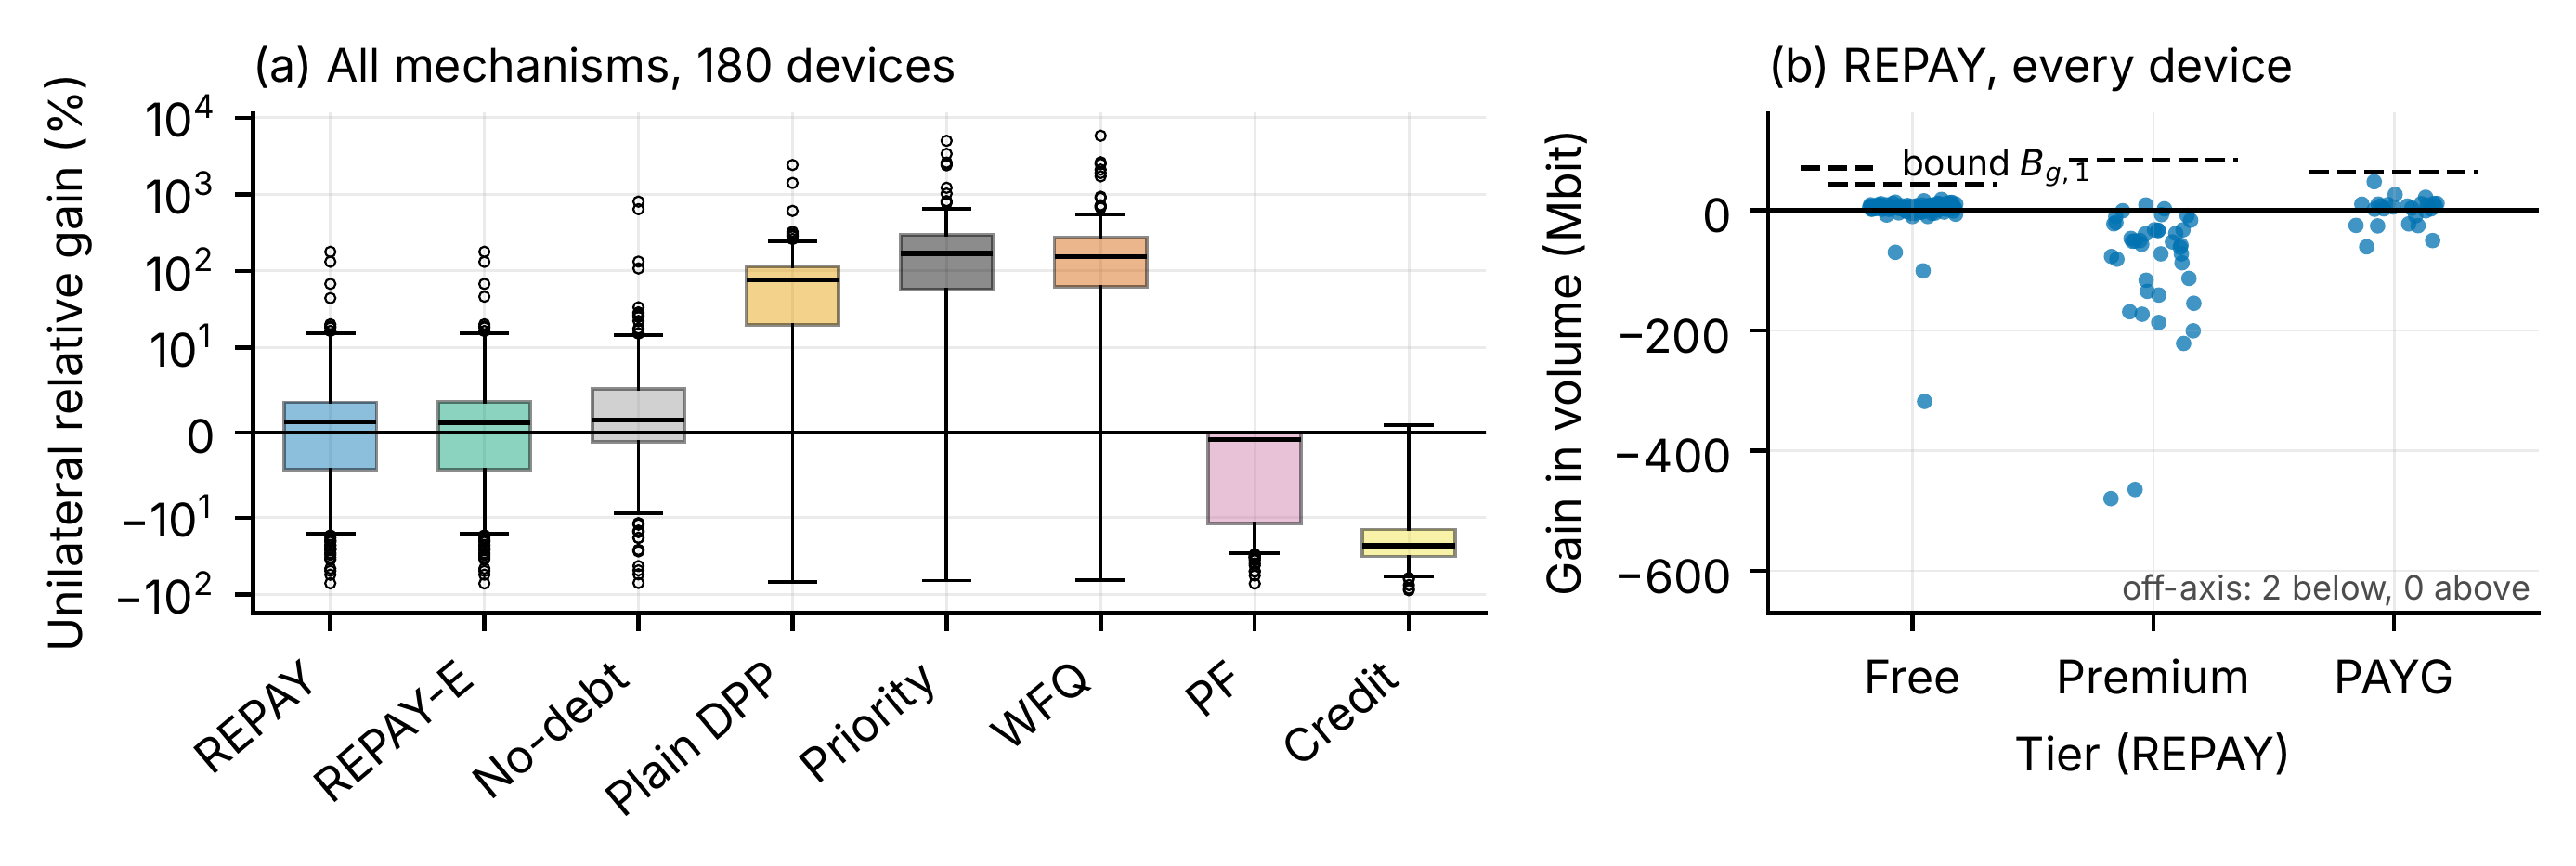
\includegraphics[width=\linewidth]{fig_deviation.png}
\caption{Unilateral misreport. Left: gain per slot for each rule. Right: gain in volume under \repay{} compared with the bound.}
\label{fig:deviation}
\end{figure}

\paragraph{When many misreport.}
Figure~\ref{fig:collapse} lets a fraction $\rho$ of the elastic devices declare video.
Under \textsc{Priority}, \textsc{WFQ} and plain DPP a misreporting device receives more than a truthful one at every interior $\rho$ we tested ($0.25$, $0.5$, $0.75$) (for instance $1.60$ against $0.63$~Mbit/s under \textsc{Priority} at $\rho=0.25$), so $\rho$ drifts to one.
At $\rho=1$ the rules have nothing left to differentiate on. \textsc{WFQ} then serves $78\%$ of genuine RT slots, the same as \textsc{PF}, and plain DPP $88\%$, the same as \repay{}, which has no elastic device left to owe anything to; total utility falls from $72.3$ to $59.8$ under \textsc{WFQ} and from $73.2$ to $63.2$ under plain DPP.
\textsc{Priority} with admission control degrades more gracefully: it still serves $95.8\%$ of genuine RT slots at $\rho=1$, because it admits flows at the minimum rate, but calls then run at lower quality (video utility $1.75$ per slot instead of $2.53$) and every elastic device, capped at the video rate, receives $0.97$~Mbit/s.
Under \repay{} a misreporting device receives \emph{less} than a truthful one ($1.08$ against $1.23$~Mbit/s at $\rho=0.25$), so in these runs no device has a reason to leave the truthful profile $\rho=0$. Part of this sign is due to the cap of the video bundle: under class-blind \textsc{PF}, where the declaration has no other effect, misreporters receive $0.26$~Mbit/s less than truthful devices, against $0.15$ less under \repay{}. (In this paragraph the rate of an elastic device is its volume divided by the length of its stay, idle periods included, hence the lower values than in Table~\ref{tab:compare}.)
Comparing the points where each rule comes to rest, \repay{} at $\rho=0$ delivers a utility of $70.9$, an elastic rate of $1.27$~Mbit/s and a video utility of $1.92$, against $64.9$, $0.97$ and $1.75$ for \textsc{Priority} at $\rho=1$.
The two serve almost the same share of genuine RT slots ($94.7\%$ for \repay{} and $95.8\%$ for \textsc{Priority}), and \textsc{Priority} does so with an elastic rate that is $24\%$ lower.

\begin{figure}[t]
\centering
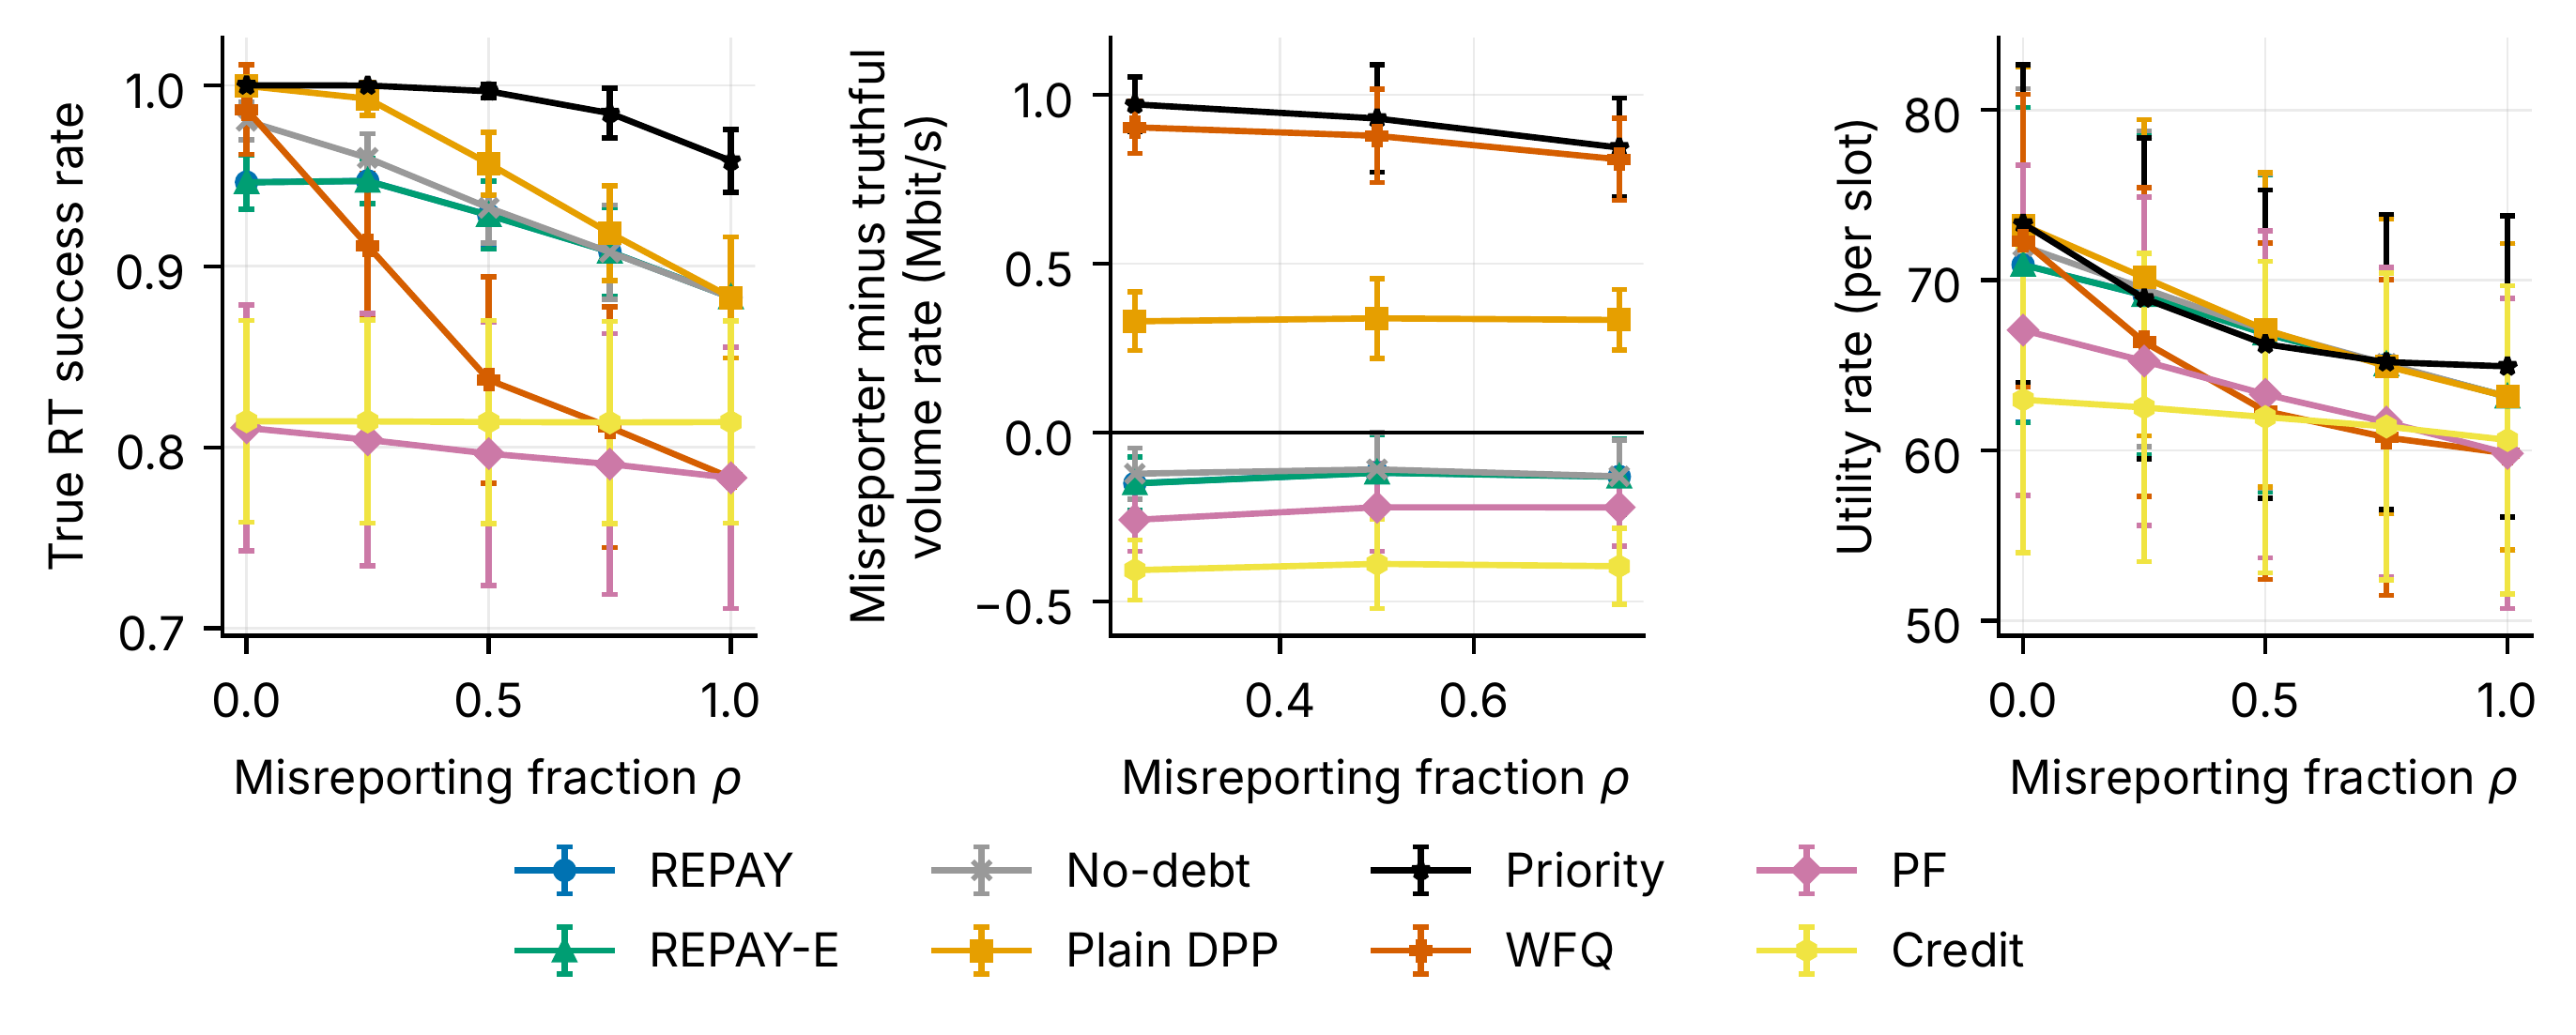
\includegraphics[width=\linewidth]{fig_collapse.png}
\caption{A fraction $\rho$ of elastic devices declares video. Left: success of genuine RT flows. Middle: rate of misreporting minus rate of truthful elastic devices (positive values mean that misreporting pays). Right: total utility.}
\label{fig:collapse}
\end{figure}

\paragraph{The reverse deviation.}
We also let $40$ video devices declare elastic, under \repay{} and under plain DPP.
Every one of them loses utility (on average $38$ utility units over its stay under \repay{}), consistent with Proposition~\ref{prop:reverse}, which covers one slot without outstanding deficits.

\paragraph{Switching strategies.}
Finally we test dynamic declarations, on $120$ elastic devices that stay at least $200$ slots ($20$ on each of six traces).
The first attacker declares video whenever capacity is below its 40th percentile and elastic otherwise, subject to a hold-down of $\tau$ slots (Figure~\ref{fig:switching}).
Under plain DPP this strategy gains $0.18$ to $0.25$~Mbit/s for every $\tau$.
Under \repay{} it loses $0.02$ to $0.05$~Mbit/s on average, the best single device gains $0.06$~Mbit/s, and no device exceeds the bound $KB$ of Theorem~\ref{thm:dynamic}.
The second attacker is an oracle built to exploit Proposition~\ref{prop:commit}: it observes, on the truthful path, the slots in which its video reference exceeds its own allocation, and declares video exactly in those slots, again subject to a hold-down.
Under the price-taking hypothesis this strategy would gain $24$ to $40$~Mbit per device.
In the actual system it loses (Table~\ref{tab:oracle}): the mean change is between $-0.035$ and $-0.053$~Mbit/s for $\tau$ from $1$ to $60$, and at most $24\%$ of the devices gain anything, the largest gain being $0.06$~Mbit/s.
One rule of the implementation that the price-taking calculation ignores works against the attacker: a device that leaves the elastic class forfeits its deficits and restarts from zero when it returns.
Table~\ref{tab:ablation} isolates it on two of the traces. If deficits are instead kept frozen while the device poses as video, the attack becomes profitable for most devices at $\tau=1$ ($95\%$ of them gain), though by little: $0.016$~Mbit/s on average, about $1.4\%$ of their volume, and at most $0.09$~Mbit/s for any device at any $\tau$. Admitting incumbents first in addition changes nothing material.
Forfeiture is thus what makes slot-by-slot switching unprofitable in these runs (two traces; without it the mean gain is positive at $\tau=1$ and $\tau=5$ and negative at $\tau=20$). It has a cost for an honest user who makes a call and then resumes a download: the credit accumulated before the call is lost.
The experiments therefore do not show that a hold-down is needed in practice; in these experiments it is a restriction placed on the attacker, not something the allocation code enforces. Proposition~\ref{prop:commit} says that without one there is no guarantee, and we keep it as a safeguard.

\begin{figure}[t]
\centering
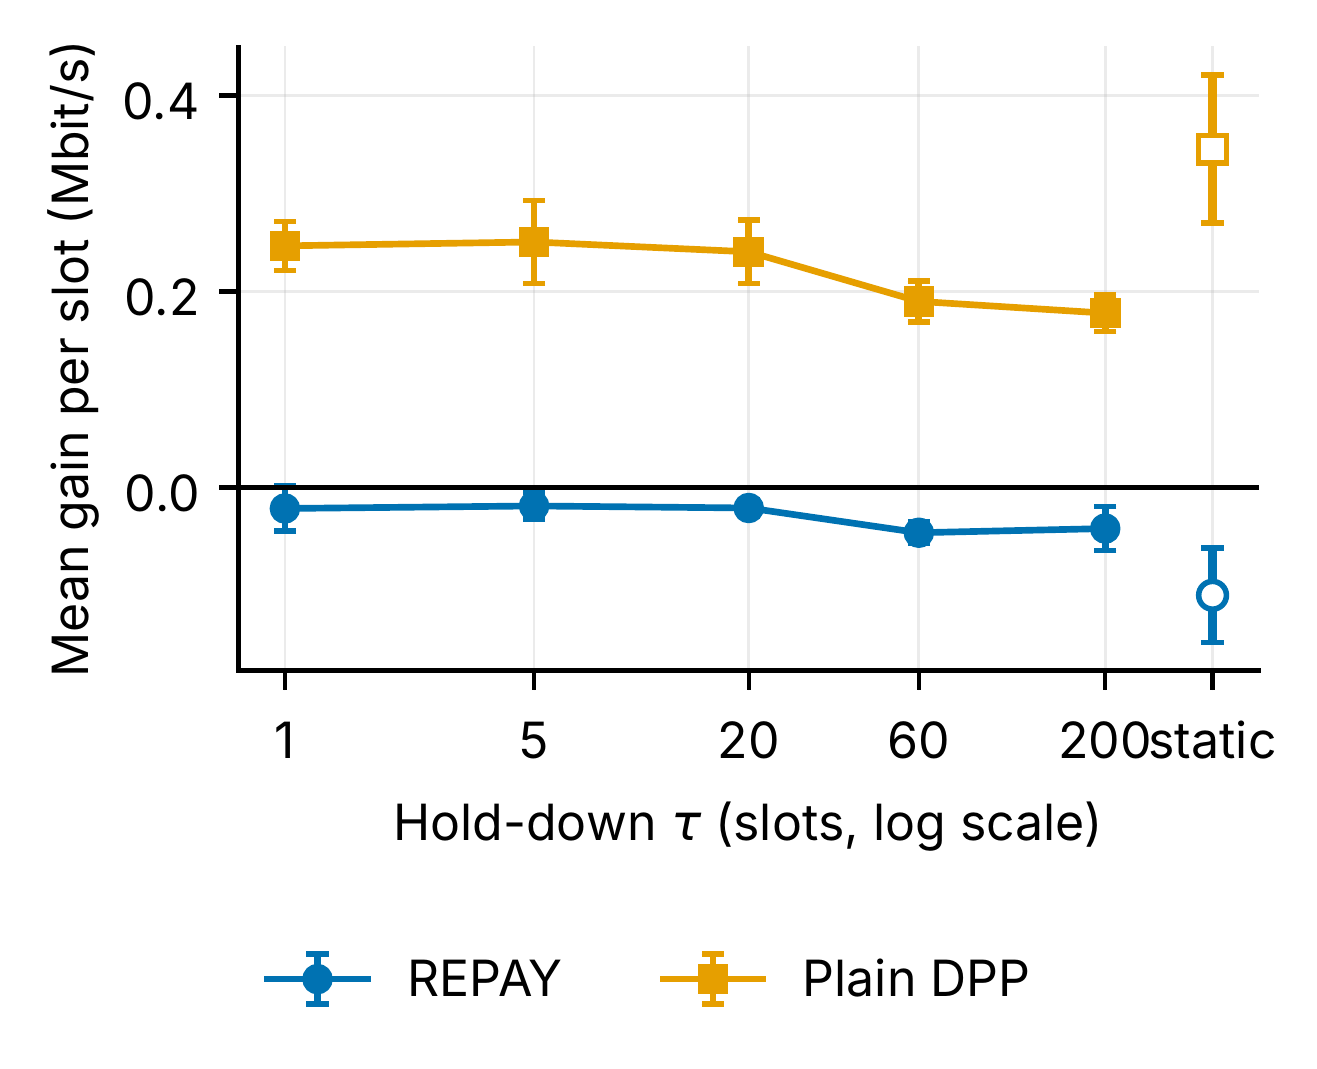
\includegraphics[width=0.45\linewidth]{fig_switching.png}
\caption{Mean gain per slot of the congestion-triggered switching strategy as a function of the hold-down $\tau$ ($120$ devices on six traces).}
\label{fig:switching}
\end{figure}

\begin{table}[t]
\centering
\caption{Oracle slot-switching attack against \repay{} ($120$ devices on six traces): change in volume relative to truthful declaration.}
\label{tab:oracle}
\resizebox{\linewidth}{!}{\begin{tabular}{rrrrrr}
\toprule
Hold-down $\tau$ & Mean gain per slot (Mbit/s) & Max gain per slot (Mbit/s) & Mean relative gain (\%) & Share with positive gain (\%) & Mean video phases \\
\midrule
1 & -0.035 & 0.062 & -3.93 & 15.0 & 58.89 \\
5 & -0.051 & 0.025 & -5.05 & 5.8 & 22.66 \\
20 & -0.046 & 0.048 & -3.80 & 6.7 & 8.40 \\
60 & -0.053 & 0.055 & -2.98 & 24.2 & 3.42 \\
\bottomrule
\end{tabular}}
\end{table}

\begin{table}[t]
\centering
\caption{Oracle attack ($40$ devices on two traces) against \repay{}, against a variant in which deficits are kept frozen while a device declares video, and against that variant with incumbents-first admission.}
\label{tab:ablation}
\resizebox{\linewidth}{!}{\begin{tabular}{llrrr}
\toprule
Rule & Hold-down $\tau$ & Mean gain per slot (Mbit/s) & Max gain per slot (Mbit/s) & Share gaining (\%) \\
\midrule
REPAY & 1 & -0.044 & 0.044 & 7.5 \\
REPAY & 5 & -0.056 & 0.019 & 5.0 \\
REPAY & 20 & -0.048 & 0.038 & 7.5 \\
\midrule
REPAY-keep & 1 & 0.016 & 0.072 & 95.0 \\
REPAY-keep & 5 & 0.002 & 0.044 & 72.5 \\
REPAY-keep & 20 & -0.009 & 0.092 & 65.0 \\
\midrule
REPAY-keep-sticky & 1 & 0.015 & 0.072 & 92.5 \\
REPAY-keep-sticky & 5 & 0.001 & 0.044 & 70.0 \\
REPAY-keep-sticky & 20 & -0.011 & 0.090 & 62.5 \\
\bottomrule
\end{tabular}}
\end{table}

\subsection{Traffic mix and population size}\label{sec:exp-mix}

The comparisons so far use one traffic mix, in which $35\%$ of the devices are real-time, and about $75$ devices.
We vary both on the hotspot scenario with truthful devices.
First, the real-time share $\rho_{\mathrm{RT}}$ takes the values $5$, $10$, $20$, $35$ and $50\%$, split between video and gaming in the ratio $5:2$ of the default (five traces per value).
Second, at the default mix, the arrival rate, the batch size and the mean capacity are multiplied together by $0.25$, $0.5$, $1$, $2$ and $4$, so that the load per device is unchanged and between $19$ and $288$ devices are present on average (three traces per value).
Third, at $\rho_{\mathrm{RT}}=10\%$ we repeat the unilateral deviation of Section~\ref{sec:exp-strategic} for $60$ elastic devices on two traces.

Figure~\ref{fig:mix} shows the first sweep.
\repay{} serves between $91.1\%$ and $95.1\%$ of RT slots at every share, with class envy between $5$ and $18$~Mbit and an elastic rate between $1.65$ and $1.72$~Mbit/s, close to that of \textsc{PF} ($1.67$ to $1.79$).
\textsc{Priority} serves all RT slots at every share, with class envy above $2000$~Mbit; plain DPP serves at least $99.4\%$ with class envy above $1000$~Mbit.
Capped priority with $q=0.3$ changes character with the mix: when real-time devices are few the cap does not bind, and it behaves like strict priority ($100\%$ of RT slots, class envy of $2070$~Mbit at $\rho_{\mathrm{RT}}=5\%$), and when they are many it rations them ($86.7\%$ of RT slots at $\rho_{\mathrm{RT}}=50\%$, with an elastic rate of $2.32$~Mbit/s).
Table~\ref{tab:mix-dev} gives the corresponding incentives at $\rho_{\mathrm{RT}}=10\%$: under capped priority the median misreporting device gains $113\%$ and $82\%$ of the devices gain, close to \textsc{WFQ} ($133\%$) and \textsc{Priority} ($145\%$), while under \repay{} the median change is $-0.9\%$, $45\%$ of the devices gain and none exceeds its bound (the largest gain is $0.19$ of it).
Without the debt price the median gain is $3.4\%$, $75\%$ of the devices gain and three of the $60$ exceed the bound, by up to a factor $1.75$.

The population sweep (Table~\ref{tab:mix-scale}) shows no degradation with size: \repay{} serves between $92.9\%$ and $95.5\%$ of RT slots from $19$ to $288$ devices, its class envy decreases from $19$ to $13$~Mbit, and its elastic rate stays within $0.06$~Mbit/s of that of \textsc{PF}.
This is the experiment in which the unnormalised tier queues of the earlier version failed (Section~\ref{sec:algorithm}).

\begin{figure}[t]
\centering
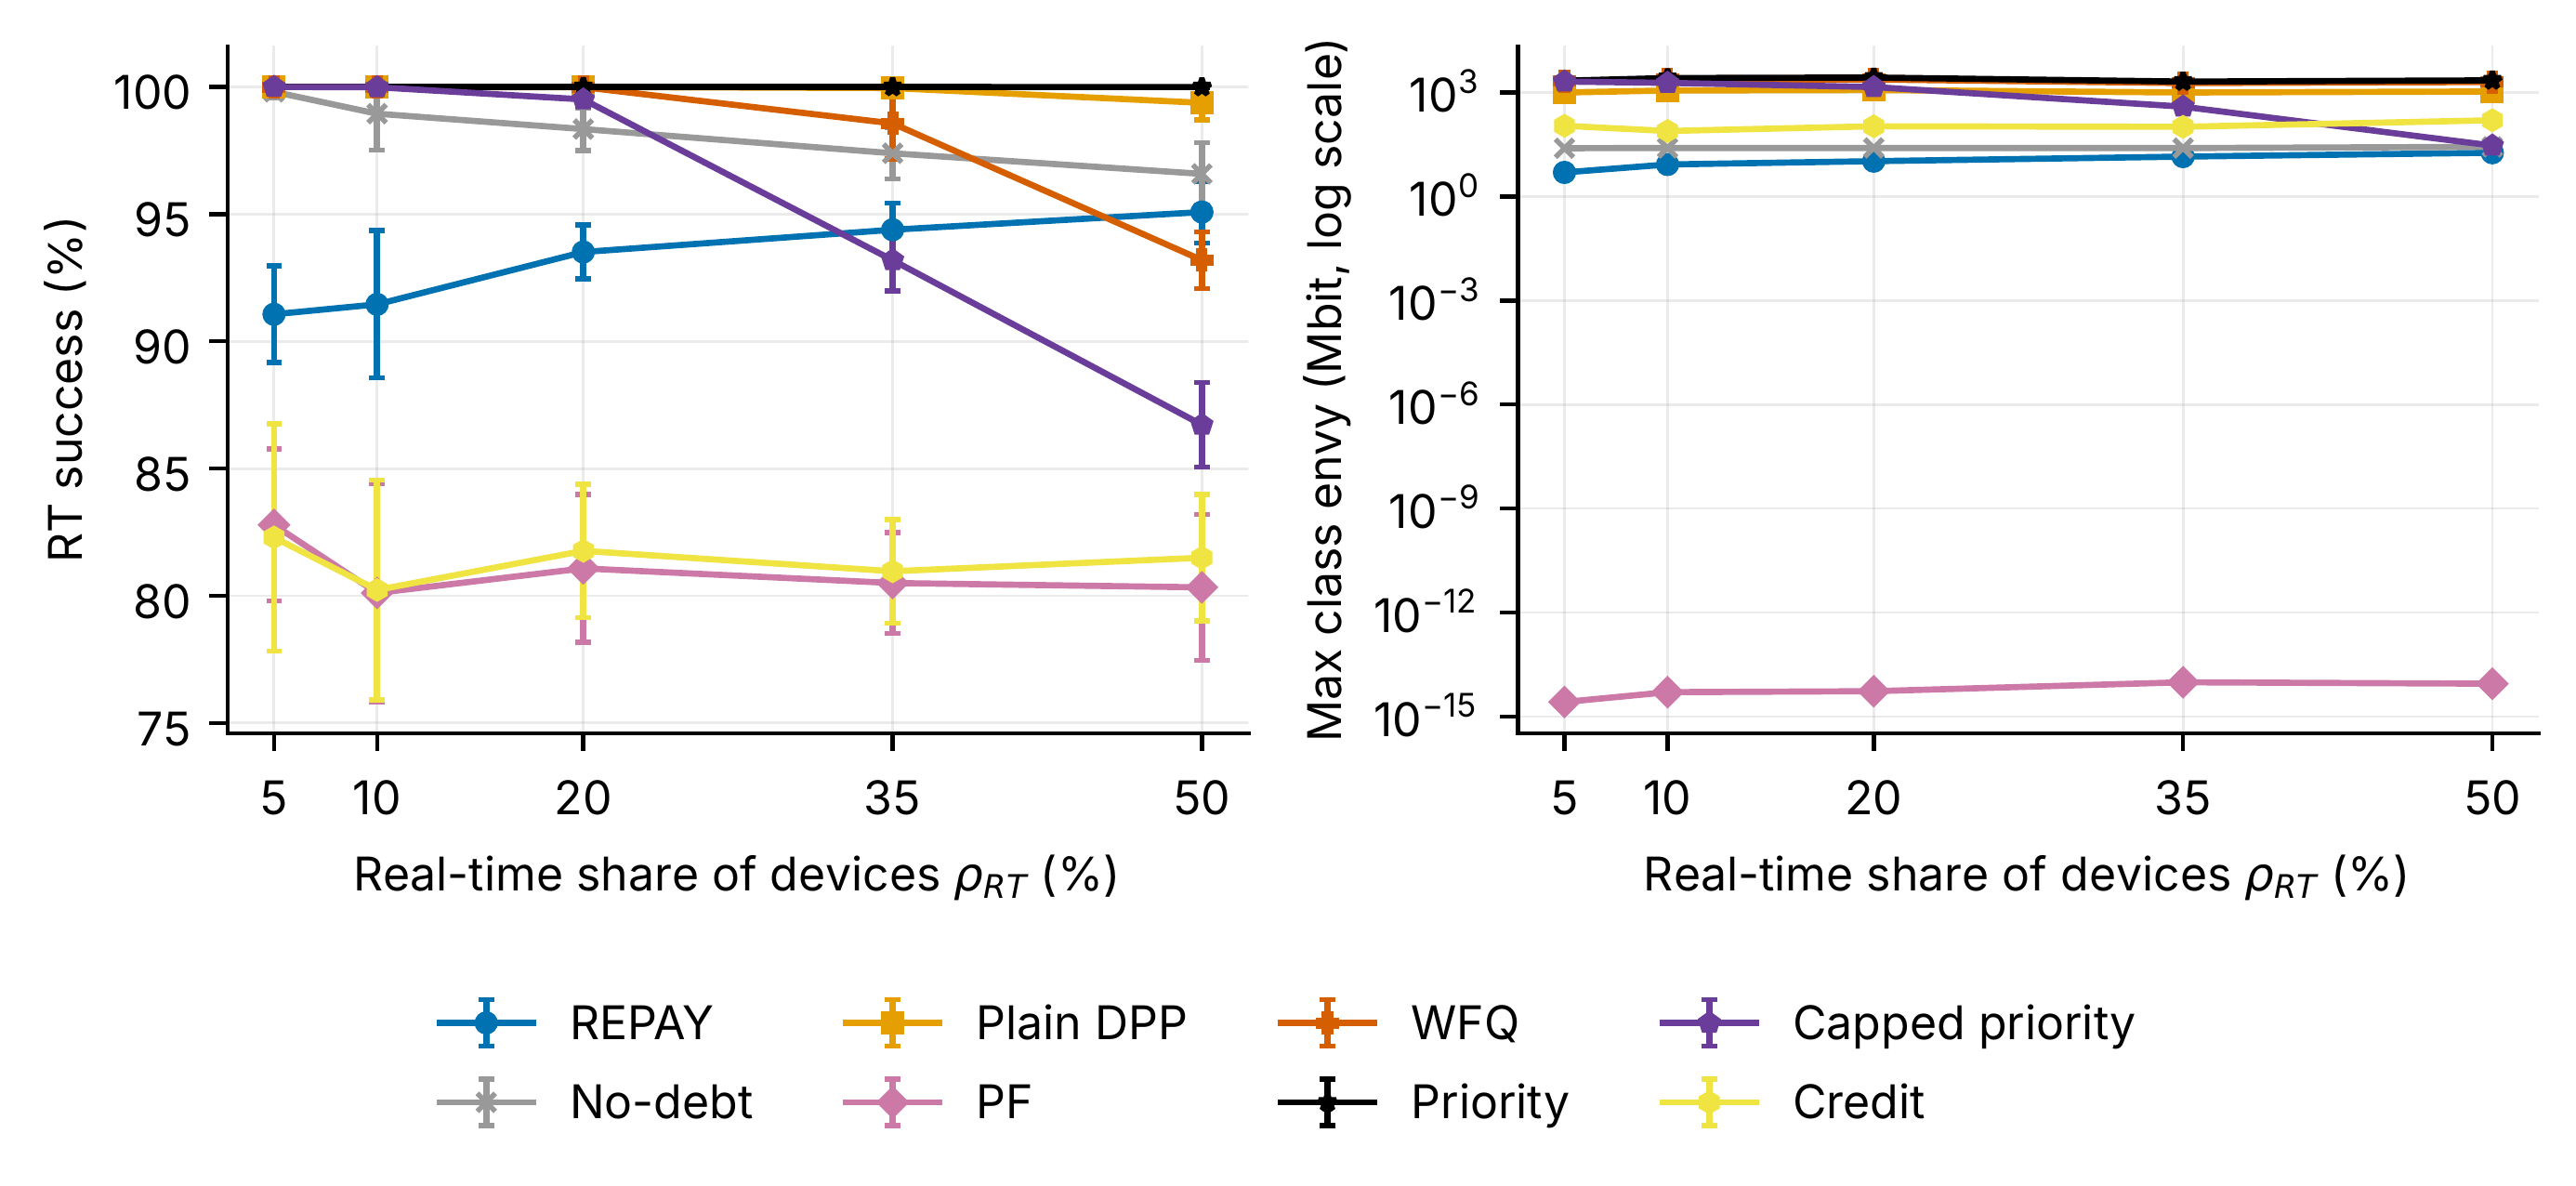
\includegraphics[width=\linewidth]{fig_mix.png}
\caption{Hotspot scenario with truthful devices, varying the share of real-time devices (mean over five traces): (a) RT success, (b) maximum class envy (logarithmic scale; \textsc{PF} has none).}
\label{fig:mix}
\end{figure}

\begin{table}[t]
\centering
\caption{RT success (\%) when the population is scaled at the default mix (columns: mean number of devices present; mean over three traces $\pm$ half-width of the 95\% interval).}
\label{tab:mix-scale}
\resizebox{\linewidth}{!}{\begin{tabular}{lrrrrr}
\toprule
Mechanism & 19 & 37 & 75 & 146 & 288 \\
\midrule
REPAY & 92.9 $\pm$ 4.8 & 94.7 $\pm$ 2.8 & 94.1 $\pm$ 1.7 & 95.5 $\pm$ 2.9 & 95.4 $\pm$ 2.6 \\
No-debt & 95.1 $\pm$ 3.7 & 97.6 $\pm$ 1.9 & 96.9 $\pm$ 1.1 & 98.7 $\pm$ 1.7 & 98.5 $\pm$ 1.5 \\
Plain DPP & 97.9 $\pm$ 3.3 & 99.7 $\pm$ 0.4 & 99.9 $\pm$ 0.1 & 100.0 $\pm$ 0.0 & 100.0 $\pm$ 0.0 \\
PF & 81.2 $\pm$ 8.1 & 80.1 $\pm$ 8.2 & 81.1 $\pm$ 4.5 & 82.4 $\pm$ 4.3 & 82.2 $\pm$ 3.3 \\
WFQ & 96.5 $\pm$ 3.1 & 97.3 $\pm$ 2.4 & 98.2 $\pm$ 3.4 & 99.5 $\pm$ 0.4 & 99.7 $\pm$ 0.1 \\
Priority & 100.0 $\pm$ 0.0 & 100.0 $\pm$ 0.0 & 100.0 $\pm$ 0.0 & 100.0 $\pm$ 0.0 & 100.0 $\pm$ 0.0 \\
Capped priority & 90.9 $\pm$ 2.1 & 91.9 $\pm$ 3.2 & 92.8 $\pm$ 2.0 & 94.7 $\pm$ 0.7 & 95.1 $\pm$ 1.1 \\
Credit & 81.8 $\pm$ 3.9 & 80.6 $\pm$ 7.2 & 81.4 $\pm$ 5.0 & 83.0 $\pm$ 3.8 & 83.1 $\pm$ 4.1 \\
\bottomrule
\end{tabular}}
\end{table}

\begin{table}[t]
\centering
\caption{Unilateral misreport at a real-time share of $10\%$ ($60$ devices on two traces). The bound is $B_{g,\mathrm{v}}$ at $V=20$ for the tier of the device; capped priority uses $q=0.3$.}
\label{tab:mix-dev}
\resizebox{\linewidth}{!}{\begin{tabular}{lrrrrr}
\toprule
Mechanism & $n$ & Median rel.\ gain (\%) & Pooled volume gain (\%) & Devices gaining (\%) & Devices above bound \\
\midrule
REPAY & 60 & -0.90 & -13.31 & 45.0 & 0 \\
No-debt & 60 & 3.37 & -5.06 & 75.0 & 3 \\
Plain DPP & 60 & 72.71 & 28.11 & 81.7 & -- \\
Priority & 60 & 144.79 & 79.78 & 90.0 & -- \\
WFQ & 60 & 133.21 & 75.17 & 90.0 & -- \\
Capped priority & 60 & 113.34 & 51.11 & 81.7 & -- \\
PF & 60 & -0.11 & -15.64 & 0.0 & -- \\
\bottomrule
\end{tabular}}
\end{table}

\subsection{Trace-driven evaluation}\label{sec:exp-real}

The experiments so far use synthetic arrivals, stays, demands, classes and capacity.
We now build them from public logs. The result is a trace-driven scenario, not the trace of one operator.

\paragraph{Construction.}
Arrivals, stays, demand levels and service classes come from the session logs that the City of Paris publishes for its public Wi-Fi network \citep{pariswifi2026}, which give, for every session, its start, its duration and the bytes and packets transferred in each direction.
We take a site with a large population (code PW0127, ``Quartier Jeunes'' in the data), the six days with the most sessions since January 2025 and, in each, the two hours with the highest occupancy; a second, smaller site (PW0232, the Petit Palais museum) serves as a check.
These are the busiest days by construction and all six are Thursdays, four of them consecutive, so the traces are not an independent sample of days.
A device is a session: the network limits connections to two hours, so a user who reconnects counts as a new device, and the roughly one hundred sessions already open at the start of a window enter with zero deficits and are observed only for the part of their stay that falls in the window.

The \emph{class} of a device is inferred from the traffic of its session.
A session is taken to be a video call if its traffic is two-way, with a ratio of uplink to downlink bytes between $1/3$ and $3$, and its mean uplink rate is at least $0.1$~Mbit/s; to be a game if it is two-way at a lower uplink rate (at least $0.01$~Mbit/s) with a mean downlink packet below $700$ bytes; and to be elastic otherwise.
This is a heuristic on session averages and not a validated classifier, so we also report a stricter rule (ratio between $1/2$ and $2$ for both classes, uplink at least $0.2$~Mbit/s for video).
Only the class is taken from the log: a device classified as real-time has the rate requirements of the model ($\rmin_{\mathrm{v}}$, $\rmax_{\mathrm{v}}$, $r_{\mathrm{g}}$), not its logged rate.
Table~\ref{tab:real-classes} gives the resulting shares: $8\%$ of the sessions of the main site are video-like and $2\%$ game-like, against the $25\%$ and $10\%$ that we assumed in the synthetic hotspot.
For an elastic device the demand cap is set so that its mean demand equals the mean downlink rate observed for its session (median cap $0.29$ to $0.52$~Mbit/s), with on--off periods as before.

The logs contain no \emph{tier}, since the network is free.
We draw tiers at random from an estimate assembled from two public figures: the connectivity sessions of a commercial in-flight Wi-Fi service equalled $11.6\%$ of its passengers in North America in 2018, sessions paid by third parties or airlines included \citep{gogo2019tenk}, which we take as a proxy for the share of paying users, and $8\%$ of mobile users in metropolitan France are on prepaid cards \citep{arcep2026mobile}, which we take as the share of pay-as-you-go among paying users.
This gives $88.4\%$ free, $10.7\%$ premium and $0.9\%$ PAYG. It is a rough estimate from unrelated markets; a variant with every device in the free tier is reported as well.

\emph{Capacity} follows the throughput logs, at roughly one sample per second, that \citet{riiser2013commute} recorded in a 3G network on metro, tram, train, bus and ferry routes in Oslo, which has nothing to do with the Paris network; we treat each sample as one slot (gaps in the logs are skipped), concatenate the logs in random order and scale them by a constant so that mean capacity is a multiple (the \emph{load}, $1$ by default) of the mean nominal demand.
Table~\ref{tab:real-traces} describes the traces.
Compared with the synthetic hotspot, about $120$ devices are present instead of $75$, the median stay in the window is $35$ to $48$ minutes instead of a mean of four minutes, real-time traffic is three times rarer, elastic demand is light, and capacity is far more variable, with a coefficient of variation of $0.70$ to $0.84$ and deep fades.
All parameters of the rules, including $V=20$ and the cap $q=0.3$, are those of the synthetic experiments and were not retuned.

\begin{table}[t]
\centering
\caption{Share of sessions classified as video-like and game-like, and median session rates of each group (sessions since January 2025).}
\label{tab:real-classes}
\resizebox{0.85\linewidth}{!}{\begin{tabular}{llrrrrr}
\toprule
Site & Rule & Share video (\%) & Share gaming (\%) & Video down (Mbit/s) & Video up (Mbit/s) & Gaming down (Mbit/s) \\
\midrule
PW0127 & default & 7.7 & 2.4 & 0.353 & 0.241 & 0.047 \\
PW0127 & strict & 3.0 & 2.3 & 0.515 & 0.460 & 0.056 \\
PW0232 & default & 12.0 & 0.5 & 0.349 & 0.322 & 0.029 \\
PW0232 & strict & 5.5 & 0.4 & 0.478 & 0.476 & 0.040 \\
\bottomrule
\end{tabular}}
\end{table}

\begin{table}[t]
\centering
\caption{Trace-driven scenario: two-hour windows of the Paris public Wi-Fi session logs, with capacity from 3G commute logs scaled to load $1$.}
\label{tab:real-traces}
\resizebox{\linewidth}{!}{\begin{tabular}{llrrrrrrrrr}
\toprule
Trace & Date & Devices & Video & Gaming & Mean conc. & Median stay (s) & Median elastic cap (Mbit/s) & 90th pct.\ elastic cap (Mbit/s) & Mean capacity (Mbit/s) & CV of capacity \\
\midrule
PW0127, $k=0$ & 2025-04-03 & 283 & 16 & 8 & 125.5 & 2677 & 0.29 & 1.26 & 51.8 & 0.72 \\
PW0127, $k=1$ & 2025-10-30 & 270 & 20 & 9 & 120.6 & 2645 & 0.35 & 1.33 & 58.7 & 0.84 \\
PW0127, $k=2$ & 2026-04-09 & 305 & 29 & 9 & 131.7 & 2535 & 0.43 & 1.54 & 71.5 & 0.74 \\
PW0127, $k=3$ & 2026-04-16 & 226 & 19 & 3 & 88.1 & 2078 & 0.52 & 1.81 & 53.8 & 0.70 \\
PW0127, $k=4$ & 2026-04-23 & 272 & 23 & 9 & 113.2 & 2407 & 0.40 & 1.88 & 66.0 & 0.75 \\
PW0127, $k=5$ & 2026-04-30 & 295 & 28 & 10 & 131.4 & 2880 & 0.41 & 1.77 & 70.9 & 0.70 \\
\midrule
PW0232, mean of $k=0,\dots,5$ & -- & 153.7 & 25.7 & 1.3 & 37.3 & 1288 & 0.58 & 2.01 & 26.5 & 0.74 \\
\bottomrule
\end{tabular}}
\end{table}

\begin{table}[t]
\centering
\caption{Trace-driven scenario, site PW0127, load $1$, truthful devices (mean over six traces $\pm$ half-width of the 95\% interval). The premium target is $0.8$.}
\label{tab:real-compare}
\resizebox{\linewidth}{!}{\begin{tabular}{lrrrrrr}
\toprule
Mechanism & Utility & RT success (\%) & Video success (\%) & Elastic rate (Mbit/s) & Max class envy (Mbit) & Premium served ratio \\
\midrule
REPAY & 44.82 $\pm$ 7.06 & 82.4 $\pm$ 4.4 & 79.0 $\pm$ 3.7 & 0.44 $\pm$ 0.08 & 43.92 $\pm$ 12.97 & 1.02 $\pm$ 0.11 \\
No-debt & 45.24 $\pm$ 7.16 & 90.0 $\pm$ 3.0 & 87.2 $\pm$ 3.1 & 0.44 $\pm$ 0.08 & 46.12 $\pm$ 15.54 & 0.92 $\pm$ 0.09 \\
Plain DPP & 46.47 $\pm$ 7.27 & 96.2 $\pm$ 1.8 & 95.3 $\pm$ 2.0 & 0.39 $\pm$ 0.08 & 2556.78 $\pm$ 301.64 & 1.04 $\pm$ 0.12 \\
PF & 43.47 $\pm$ 6.87 & 75.4 $\pm$ 4.9 & 73.2 $\pm$ 4.6 & 0.44 $\pm$ 0.08 & 0.00 $\pm$ 0.00 & 1.04 $\pm$ 0.08 \\
WFQ & 44.80 $\pm$ 6.97 & 94.1 $\pm$ 1.6 & 93.6 $\pm$ 1.6 & 0.32 $\pm$ 0.07 & 5088.25 $\pm$ 1132.22 & 0.99 $\pm$ 0.20 \\
Priority & 45.13 $\pm$ 7.11 & 97.1 $\pm$ 1.2 & 96.6 $\pm$ 1.4 & 0.32 $\pm$ 0.07 & 5356.58 $\pm$ 1313.04 & 0.91 $\pm$ 0.19 \\
Capped priority ($q=0.3$) & 45.24 $\pm$ 7.01 & 91.3 $\pm$ 2.1 & 89.8 $\pm$ 2.3 & 0.43 $\pm$ 0.07 & 1159.08 $\pm$ 443.83 & 0.92 $\pm$ 0.04 \\
Credit & 40.36 $\pm$ 6.41 & 58.8 $\pm$ 6.5 & 50.2 $\pm$ 4.4 & 0.47 $\pm$ 0.08 & 167.45 $\pm$ 163.49 & 0.87 $\pm$ 0.06 \\
\bottomrule
\end{tabular}}
\end{table}

\begin{table}[t]
\centering
\caption{Trace-driven scenario, site PW0127: RT success and elastic rate at three loads (mean over six traces).}
\label{tab:real-load}
\resizebox{\linewidth}{!}{\begin{tabular}{lrrrrrr}
\toprule
 & \multicolumn{3}{c}{RT success (\%)} & \multicolumn{3}{c}{Elastic rate (Mbit/s)} \\
\cmidrule(lr){2-4}\cmidrule(lr){5-7}
Mechanism & 0.7 & 1.0 & 1.5 & 0.7 & 1.0 & 1.5 \\
\midrule
REPAY & 73.9 & 82.4 & 88.3 & 0.37 & 0.44 & 0.50 \\
No-debt & 84.3 & 90.0 & 93.5 & 0.37 & 0.44 & 0.51 \\
Plain DPP & 94.5 & 96.2 & 97.6 & 0.31 & 0.39 & 0.47 \\
PF & 63.5 & 75.4 & 83.4 & 0.37 & 0.44 & 0.51 \\
WFQ & 91.7 & 94.1 & 95.9 & 0.21 & 0.32 & 0.43 \\
Priority & 95.9 & 97.1 & 98.0 & 0.20 & 0.32 & 0.43 \\
Capped priority ($q=0.3$) & 88.0 & 91.3 & 93.9 & 0.36 & 0.43 & 0.50 \\
Credit & 44.1 & 58.8 & 73.1 & 0.40 & 0.47 & 0.52 \\
\bottomrule
\end{tabular}}
\end{table}

\begin{table}[t]
\centering
\caption{Trace-driven scenario, site PW0127, load $1$: sensitivity to the classification rule and to the tier assumption.}
\label{tab:real-variants}
\resizebox{\linewidth}{!}{\begin{tabular}{lrrrrrr}
\toprule
 & \multicolumn{3}{c}{strict rule} & \multicolumn{3}{c}{all devices free} \\
\cmidrule(lr){2-4}\cmidrule(lr){5-7}
Mechanism & RT success (\%) & Elastic rate (Mbit/s) & Max class envy (Mbit) & RT success (\%) & Elastic rate (Mbit/s) & Max class envy (Mbit) \\
\midrule
REPAY & 87.3 $\pm$ 2.9 & 0.44 $\pm$ 0.08 & 15.29 $\pm$ 3.81 & 83.7 $\pm$ 3.6 & 0.45 $\pm$ 0.07 & 56.00 $\pm$ 14.80 \\
No-debt & 94.2 $\pm$ 1.7 & 0.44 $\pm$ 0.08 & 45.70 $\pm$ 15.10 & 90.4 $\pm$ 2.6 & 0.45 $\pm$ 0.07 & 34.84 $\pm$ 3.65 \\
Plain DPP & 98.4 $\pm$ 1.2 & 0.42 $\pm$ 0.08 & 2299.79 $\pm$ 431.29 & 97.1 $\pm$ 1.2 & 0.40 $\pm$ 0.07 & 2664.79 $\pm$ 233.44 \\
PF & 79.8 $\pm$ 5.4 & 0.44 $\pm$ 0.08 & 0.00 $\pm$ 0.00 & 76.1 $\pm$ 4.2 & 0.45 $\pm$ 0.07 & 0.00 $\pm$ 0.00 \\
WFQ & 97.3 $\pm$ 2.0 & 0.40 $\pm$ 0.08 & 4226.98 $\pm$ 907.16 & 95.0 $\pm$ 2.0 & 0.32 $\pm$ 0.07 & 5367.10 $\pm$ 1073.94 \\
Priority & 98.6 $\pm$ 1.0 & 0.40 $\pm$ 0.08 & 4433.03 $\pm$ 915.53 & 97.1 $\pm$ 1.2 & 0.32 $\pm$ 0.07 & 5363.43 $\pm$ 1073.40 \\
Capped priority ($q=0.3$) & 95.6 $\pm$ 2.2 & 0.42 $\pm$ 0.08 & 3194.39 $\pm$ 363.56 & 91.5 $\pm$ 2.2 & 0.43 $\pm$ 0.07 & 991.82 $\pm$ 365.81 \\
Credit & 71.4 $\pm$ 4.5 & 0.45 $\pm$ 0.08 & 284.40 $\pm$ 161.43 & 59.0 $\pm$ 5.3 & 0.47 $\pm$ 0.07 & 149.32 $\pm$ 150.79 \\
\bottomrule
\end{tabular}}
\end{table}

\begin{table}[t]
\centering
\caption{Trace-driven scenario, site PW0127, load $1$: one elastic device declares video for its whole stay ($120$ devices on six traces).}
\label{tab:real-dev}
\resizebox{0.9\linewidth}{!}{\begin{tabular}{lrrrrr}
\toprule
Mechanism & $n$ & Median rel.\ gain (\%) & Pooled volume gain (\%) & Devices gaining (\%) & 95th pct.\ gain (Mbit/s) \\
\midrule
REPAY & 120 & -0.36 & -0.66 & 47.5 & 0.0390 \\
Plain DPP & 120 & 27.69 & 36.60 & 100.0 & 0.4121 \\
Priority & 120 & 64.28 & 83.22 & 100.0 & 0.7362 \\
WFQ & 120 & 65.99 & 78.74 & 100.0 & 0.7270 \\
PF & 120 & 0.00 & -0.78 & 0.0 & 0.0000 \\
Capped priority ($q=0.3$) & 120 & 3.65 & 9.40 & 65.8 & 0.1815 \\
\bottomrule
\end{tabular}}
\end{table}

\paragraph{Truthful devices.}
Table~\ref{tab:real-compare} repeats the comparison of Section~\ref{sec:exp-compare}.
\repay{} serves $82.4\%$ of RT slots against $75.4\%$ for \textsc{PF}; the paired difference over the six traces is $7.0\pm0.9$ points, at an elastic rate lower by $0.004\pm0.001$~Mbit/s.
Its class envy is $44$~Mbit on average and at most $69$~Mbit, and no deficit exceeds $0.39$ of its bound in any run.
The rules that give RT flows priority serve many more RT slots than \repay{} here, whereas on the synthetic hotspot the difference was at most five points: plain DPP serves $13.8\pm3.1$ points more RT slots than \repay{}, \textsc{WFQ} $11.7\pm3.3$ and \textsc{Priority} $14.7\pm3.8$, while the elastic rate falls by $0.05$ to $0.12$~Mbit/s, that is by $11\%$ under plain DPP and $27$--$28\%$ under \textsc{WFQ} and \textsc{Priority}.
The reason is the traffic mix. When one device in ten is real-time, serving all of them first lowers the elastic rate by a similar fraction as in the synthetic hotspot ($28\%$ under \textsc{Priority} in both cases) but by less in absolute terms, and the cost is concentrated: class envy under these rules is $2600$ to $5400$~Mbit.
Capped priority with the untuned cap $q=0.3$ sits in between, with $8.9\pm3.0$ points more RT slots than \repay{} at an elastic rate that does not differ significantly ($-0.007\pm0.014$~Mbit/s) and class envy of $1160$~Mbit.
The variant without the debt price serves $7.6\pm1.8$ points more RT slots than \repay{} at the same elastic rate and with about the same class envy ($46$~Mbit).
The premium service level is met on average by every rule; \textsc{Priority} falls below the target on two of the six traces, and \textsc{WFQ} and \textsc{Credit} on one each.
The pattern is the same at loads $0.7$ and $1.5$ (Table~\ref{tab:real-load}), on the second site ($82.9\%$ for \repay{} against $76.7\%$ for \textsc{PF} and $94.1\%$ for plain DPP), under the stricter classification rule and with all devices free (Table~\ref{tab:real-variants}).

\paragraph{The role of $V$ and of the debt price.}
On these traces \repay{} gives up twelve to fifteen points of RT success relative to the priority rules, and one may ask whether a larger $V$, which loosens the envy bound, would recover them.
It does not (Table~\ref{tab:real-sweep} and Figure~\ref{fig:real-frontier}).
Between $V=5$ and $V=500$ the RT success of \repay{} rises only from $81.3\%$ to $86.9\%$, while its class envy grows from $24$ to $189$~Mbit; plain DPP stays between $95\%$ and $97\%$ over the same range.
What holds \repay{} back is the debt price, the part of the deficit that is charged to the RT group.
The variant without it (No-debt), which keeps the deficit queues and the bonus of the creditor, serves $88.0\%$ of RT slots at $V=5$ with a class envy of $19$~Mbit and $96.6\%$ at $V=500$ with $467$~Mbit: for a given level of envy it serves about seven points more RT slots than \repay{}, at the same elastic rate, and its deficits also stay below their bound (at most $0.82$ of it in any run).
Capped priority traces a similar curve when its cap is varied ($87.4\%$ at $q=0.2$ with envy of $239$~Mbit), with no bound behind it.
At equal $V$ the debt price does reduce the gain from misreporting, as the next paragraph shows, but $V$ and the debt price turn out to be substitutes for that purpose, and the cheaper instrument is a small $V$.
The variant without the debt price at $V=5$ serves $88.0\%$ of RT slots with a class envy of $19$~Mbit and leaves a median gain from misreporting of $-0.2\%$ ($45\%$ of the devices gain, three exceed the bound); the full rule at $V=20$ serves $82.4\%$ with $44$~Mbit and $-0.4\%$ ($48\%$ gain, nine exceed the bound).
On these traces the first configuration is therefore the better one on RT success and envy, at a similar incentive to misreport.
We had taken the full rule with $V=20$ as the default on the strength of the synthetic experiments, where No-debt at the same $V$ served $2.6$ more points of RT slots at a higher envy ($25$ against $15$~Mbit), and did not retune it; the traces show that this default is not the best one when real-time traffic is rare.

\begin{figure}[t]
\centering
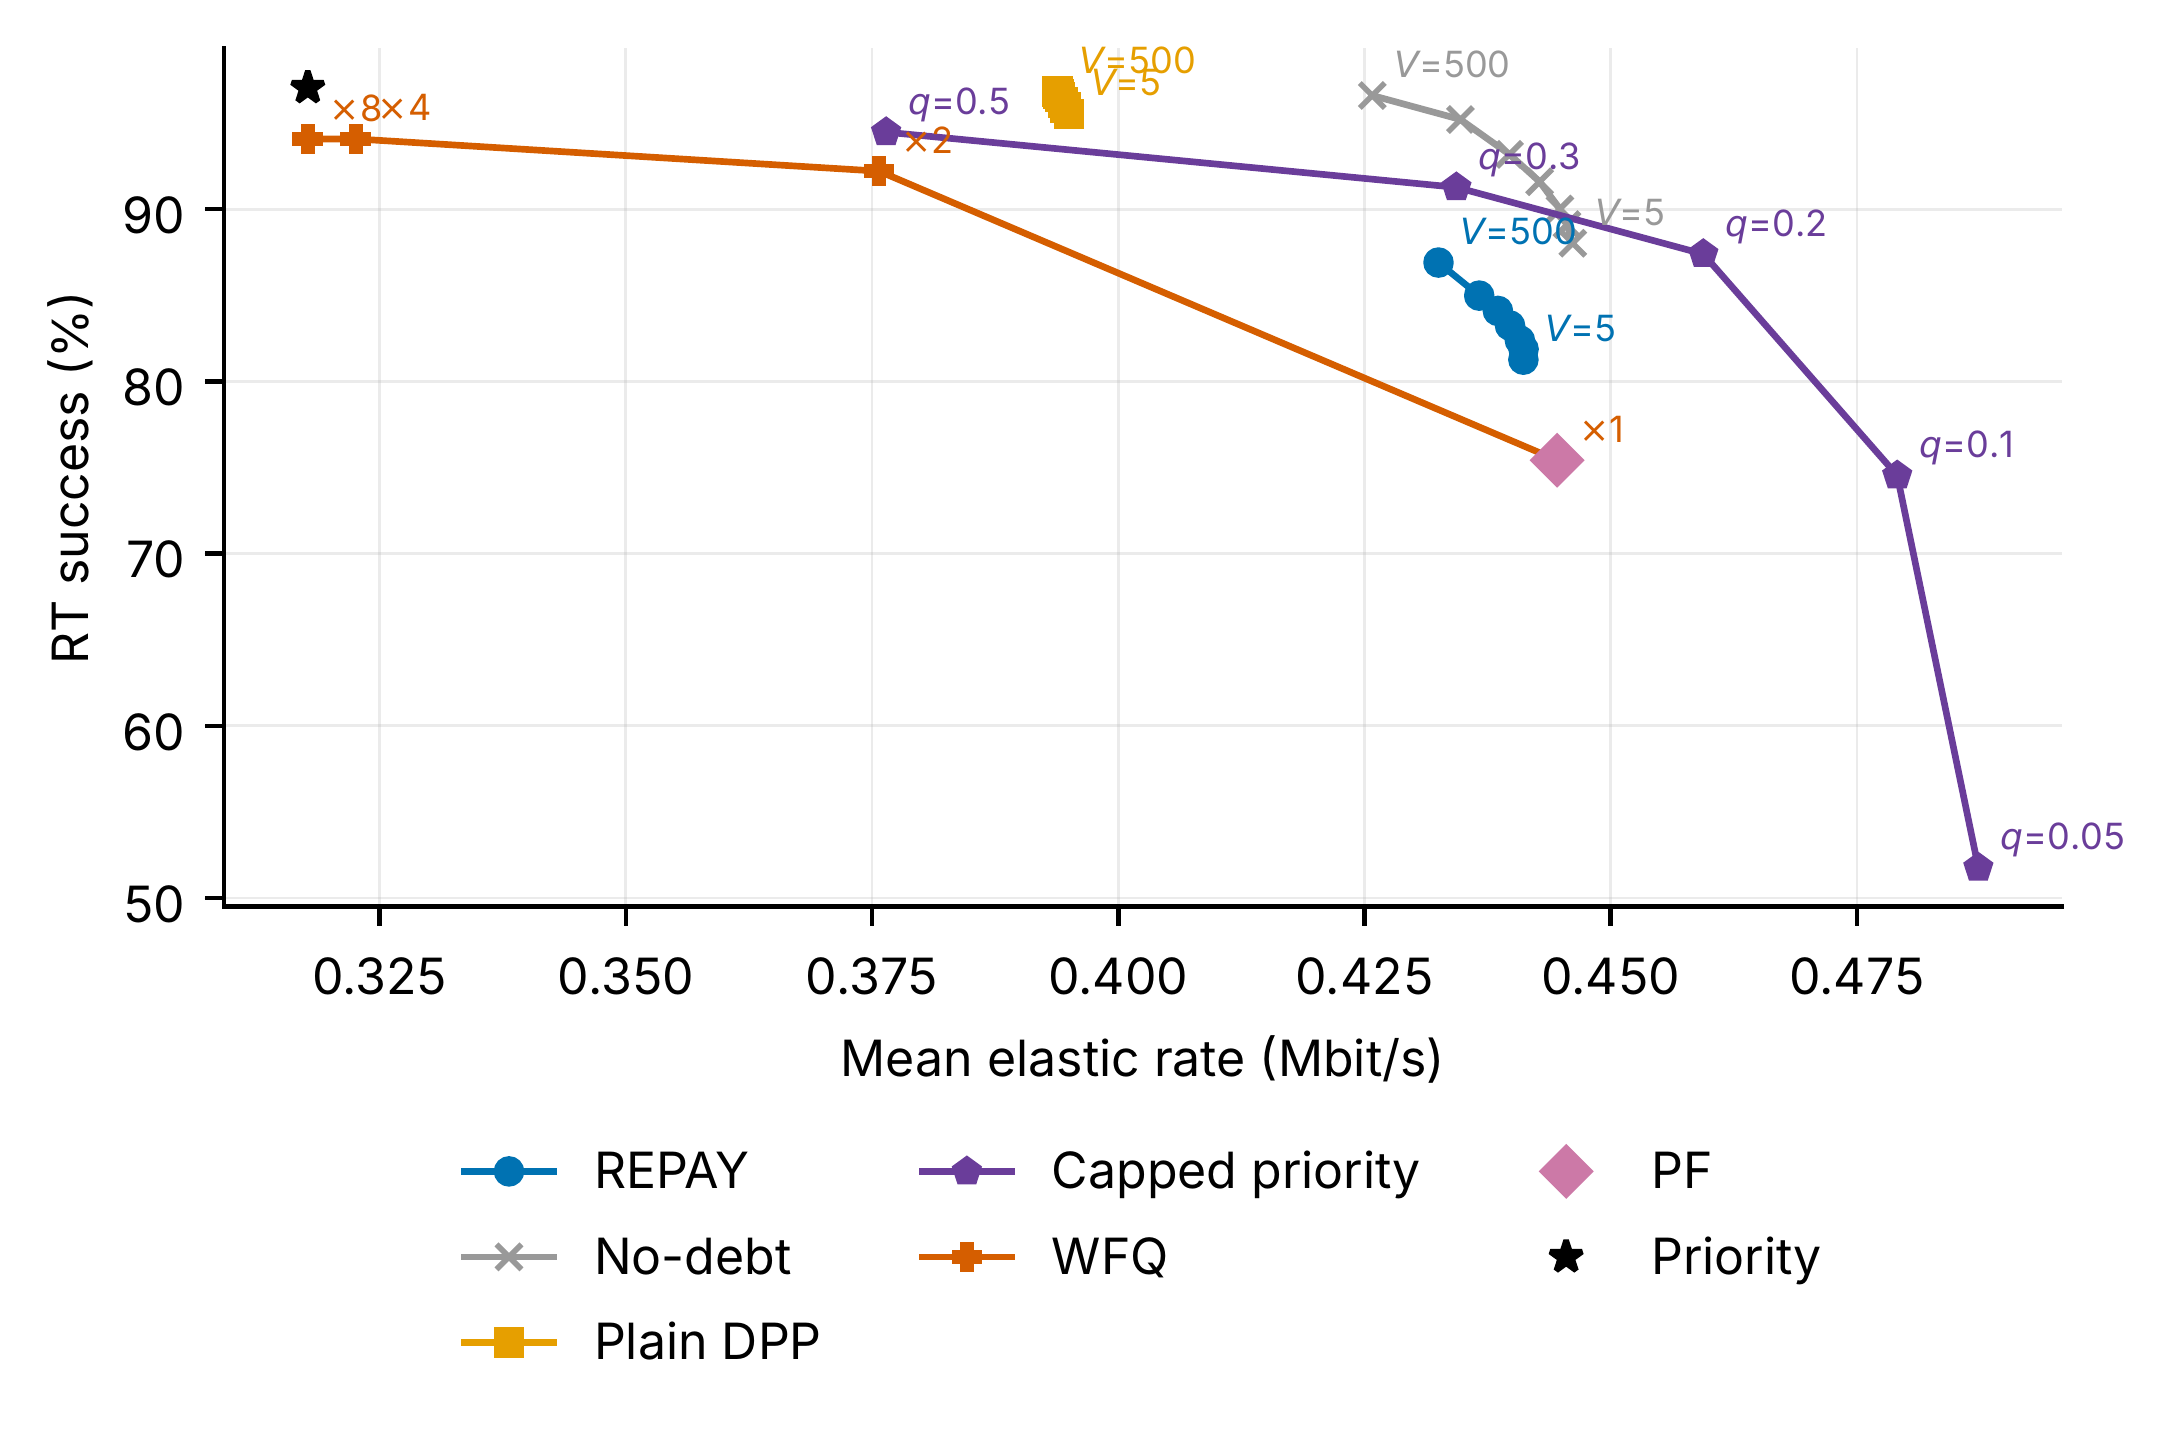
\includegraphics[width=0.75\linewidth]{fig_real_frontier.png}
\caption{Trace-driven scenario, site PW0127, load $1$: RT success against elastic rate when the parameter of each rule is varied (mean over six traces). For the families swept over $V$ only the smallest and the largest value are labelled.}
\label{fig:real-frontier}
\end{figure}

\begin{table}[t]
\centering
\caption{Trace-driven scenario: effect of $V$ (mean over six traces). The class envy reported is the largest over tiers and RT classes; the bound shown is that of the free tier and the video class, and the bounds of the premium tier and of the gaming class are larger.}
\label{tab:real-sweep}
\resizebox{0.9\linewidth}{!}{\begin{tabular}{llrrrrr}
\toprule
Mechanism & $V$ & RT success (\%) & Elastic rate (Mbit/s) & Max class envy (Mbit) & Envy bound $B$ (Mbit) & Premium served ratio \\
\midrule
REPAY & 5 & 81.3 & 0.44 & 24.12 & 13.0 & 1.025 \\
REPAY & 10 & 81.9 & 0.44 & 35.48 & 23.0 & 1.022 \\
REPAY & 20 & 82.4 & 0.44 & 43.92 & 43.0 & 1.020 \\
REPAY & 50 & 83.2 & 0.44 & 53.65 & 103.0 & 1.018 \\
REPAY & 100 & 84.1 & 0.44 & 69.43 & 203.0 & 1.019 \\
REPAY & 200 & 85.0 & 0.44 & 99.73 & 403.0 & 1.021 \\
REPAY & 500 & 86.9 & 0.43 & 189.25 & 1003.0 & 1.025 \\
\midrule
No-debt & 5 & 88.0 & 0.45 & 18.64 & 13.0 & 0.936 \\
No-debt & 10 & 89.1 & 0.45 & 30.57 & 23.0 & 0.928 \\
No-debt & 20 & 90.0 & 0.44 & 46.12 & 43.0 & 0.921 \\
No-debt & 50 & 91.6 & 0.44 & 77.26 & 103.0 & 0.910 \\
No-debt & 100 & 93.2 & 0.44 & 122.87 & 203.0 & 0.904 \\
No-debt & 200 & 95.2 & 0.43 & 234.89 & 403.0 & 0.908 \\
No-debt & 500 & 96.6 & 0.43 & 467.00 & 1003.0 & 0.937 \\
\midrule
Plain DPP & 5 & 95.5 & 0.39 & 2525.02 & -- & 1.049 \\
Plain DPP & 10 & 95.9 & 0.39 & 2542.32 & -- & 1.044 \\
Plain DPP & 20 & 96.2 & 0.39 & 2556.78 & -- & 1.039 \\
Plain DPP & 50 & 96.5 & 0.39 & 2570.50 & -- & 1.033 \\
Plain DPP & 100 & 96.7 & 0.39 & 2576.73 & -- & 1.030 \\
Plain DPP & 200 & 96.8 & 0.39 & 2580.46 & -- & 1.029 \\
Plain DPP & 500 & 96.8 & 0.39 & 2582.72 & -- & 1.027 \\
\bottomrule
\end{tabular}}
\end{table}

\begin{table}[t]
\centering
\caption{Trace-driven scenario: unilateral misreport under \repay{} and under the variant without the debt price, for several $V$ ($120$ devices on six traces). The bound is $B_{g,\mathrm{v}}$ at that $V$ for the tier of the device.}
\label{tab:real-sweep-dev}
\resizebox{0.9\linewidth}{!}{\begin{tabular}{lrrrrrr}
\toprule
Rule & $V$ & Median rel.\ gain (\%) & Pooled volume gain (\%) & Devices gaining (\%) & Devices above bound & Max gain / bound \\
\midrule
REPAY (ref.) & 20 & -0.36 & -0.66 & 47.5 & 9 & 11.638 \\
\midrule
REPAY & 5 & -1.38 & -1.46 & 37.5 & 13 & 36.091 \\
REPAY & 50 & 0.68 & 0.20 & 55.8 & 1 & 5.046 \\
REPAY & 100 & 1.34 & 1.29 & 63.3 & 1 & 2.668 \\
REPAY & 200 & 2.76 & 3.11 & 75.0 & 1 & 1.473 \\
\midrule
No-debt & 5 & -0.15 & -1.02 & 45.0 & 3 & 17.762 \\
No-debt & 20 & 1.92 & 1.25 & 85.0 & 2 & 7.725 \\
No-debt & 50 & 6.86 & 3.99 & 94.2 & 2 & 4.375 \\
No-debt & 100 & 11.59 & 7.23 & 99.2 & 2 & 2.889 \\
No-debt & 200 & 20.31 & 12.02 & 100.0 & 1 & 1.794 \\
\bottomrule
\end{tabular}}
\end{table}

\paragraph{Misreporting.}
Table~\ref{tab:real-dev} repeats the unilateral deviation of Section~\ref{sec:exp-strategic} for $20$ elastic devices per trace.
Under \textsc{Priority} and \textsc{WFQ} every device gains, with a median gain of about $65\%$; under plain DPP every device gains and the median gain is $28\%$; under capped priority $66\%$ of the devices gain, with a median of $3.7\%$.
Under \repay{} the median change is $-0.4\%$, the pooled change $-0.7\%$, and $48\%$ of the sampled devices gain something from this one deviation.

The bound of Theorem~\ref{thm:static} is exceeded, however, by $9$ of the $120$ devices.
Eight of them are in the free tier and gain between $1.07$ and $1.82$ times $B_{F,\mathrm{v}}$, that is $46$ to $78$~Mbit or $2.5$ to $13\%$ of their volume, over stays of twenty minutes to two hours in the window.
The ninth is a premium device that gains $966$~Mbit, almost twelve times its bound and $16\%$ of its volume.
The premium tier of that trace has $25$ devices and two video flows, so the device is often the only video flow of its tier and its reference on the truthful path is zero: this is the empty-group case in which the price-taking hypothesis fails outright (Section~\ref{sec:ic}).
With the entrant offer of \textsc{Repay-E} the same device gains $222$~Mbit, still more than twice its bound.
Table~\ref{tab:real-sweep-dev} shows how these gains move with $V$ and what the debt price contributes.
Under \repay{} the median gain rises from $-1.4\%$ at $V=5$ and $-0.4\%$ at $V=20$ to $2.8\%$ at $V=200$, and the share of devices that gain from $38\%$ to $75\%$.
Without the debt price the gain is larger at every $V$: the median is $-0.2\%$ at $V=5$ ($45\%$ of the devices gain), $1.9\%$ at $V=20$ ($85\%$) and $20\%$ at $V=200$, where every device gains and the figure approaches the $28\%$ of plain DPP.
The number of devices above the bound moves the other way, because the bound shrinks with $V$: thirteen under \repay{} and three without the debt price at $V=5$, and one or two for $V\ge50$.
None of this contradicts the theorem, whose hypothesis is not satisfied, and every deficit stays below its bound as Theorem~\ref{thm:bound} requires; but it shows that in thin tiers and over long stays the incentive guarantee is weaker than the bound suggests, and that the gains, although small relative to those under the other class-aware rules, are not confined to the constant $B$.

\subsection{Two further trace-driven scenarios}\label{sec:exp-real2}

To see whether these findings depend on the Paris logs and the Oslo capacity traces, we build two further scenarios from other public sources, with the same construction: the busiest two-hour window of each of the six busiest days, sessions as devices, the same class heuristic, tiers drawn from the same estimate, the same rule for elastic demand caps, and capacity scaled to load $1$ (Table~\ref{tab:real2-traces}).

\paragraph{Construction.}
The first scenario takes its sessions from the RADIUS accounting records of the public Wi-Fi network of the Grand Paris Sud agglomeration, 29 July to 31 August 2026 \citep{grandparissud2026wifi}, which give the start, the duration and the volume in each direction of every session.
No single site has enough concurrent sessions (the busiest averages eight in its busiest windows), so the unit is the whole intercommunal network, which reaches a mean concurrency of $26$ to $41$ in the chosen windows; it is thus a pool of many sites treated as one link, not one access point.
Capacity comes from the 4G bandwidth logs recorded in Ghent by \citet{vanderhooft2016http2}.
The second scenario takes its sessions from the per-association records of the public network of the City of Mesa, Arizona, in July 2025 \citep{mesa2026wifi}, at the site with the highest concurrency (code LI in the data, $14$ to $27$ concurrent sessions on average in the chosen windows), and its capacity from the 4G traces recorded in Cork by \citet{raca2018beyond4g}.
These logs have no packet counts, so the gaming rule cannot apply and no device is a game; $2$ to $13\%$ of the devices of a window are video-like.

These scenarios are weaker than the first in several respects.
Stays are short (median $12$ to $245$~s in the Grand Paris Sud windows and $24$ to $79$~s at Mesa), and elastic demand is very light: the median demand cap is at the floor of $0.05$~Mbit/s in four of the six Grand Paris Sud windows and in all Mesa windows, where even the 90th percentile is at most $0.08$~Mbit/s.
In the Mesa file the uplink counter is about ten times the downlink counter in total ($13\,071$ against $1242$~GB), which is unusual for a public hotspot; we take the counters as named, but a class heuristic based on the ratio of uplink to downlink is questionable there.
The Mesa start times carry no time zone and are read as Arizona local time.
Finally, the licence of the Grand Paris Sud data is not stated on its portal, the terms of use of the Mesa portal could not be retrieved, and the Ghent logs come with a request for citation but no licence; only the Cork traces carry an explicit licence (CC~BY~4.0). We use these data for simulation only and do not redistribute them.

\paragraph{Results.}
Table~\ref{tab:real2-compare} gives the truthful comparison, including the additional baselines of Section~\ref{sec:exp-baselines} and the variant without the debt price at $V=5$ suggested by the previous section.
On the Grand Paris Sud scenario the ordering is that of the Paris traces: \repay{} serves $89.3\%$ of RT slots against $84.5\%$ for \textsc{PF} (paired difference $4.8\pm1.9$ points, at an elastic rate lower by $0.003\pm0.002$~Mbit/s), the variant without the debt price at $V=5$ serves $94.0\%$ with a smaller class envy ($8$ against $16$~Mbit), and plain DPP, \textsc{WFQ} and \textsc{Priority} serve $97$--$98\%$ with an elastic rate lower by $0.02$ to $0.06$~Mbit/s and class envy of $1450$ to $2590$~Mbit.
On the Mesa scenario no rule does well: capacity is so variable (coefficient of variation $0.84$ to $1.21$) that RT success lies between $27\%$ and $61\%$ for every rule and the premium service level is missed on at least three of the six traces by every rule. \repay{} serves $54.2\%$ against $40.0\%$ for \textsc{PF} ($14.2\pm5.8$ points), \textsc{Priority} $60.5\%$, and capped priority only $26.8\%$, because its cap binds when capacity collapses; class envy is small for every rule, since elastic demand is tiny.
Table~\ref{tab:real2-dev} repeats the unilateral deviation.
On Grand Paris Sud the median change under \repay{} is $+0.08\%$ and $51\%$ of the devices gain, against $+17\%$ under \textsc{Priority} and $+3.3\%$ under plain DPP; five of the $120$ devices, all in the free tier, gain more than the bound, by $1.1$ to $2.2$ times $B_{F,\mathrm{v}}$ ($47$ to $93$~Mbit, $2$ to $5\%$ of their volume).
Without the debt price at $V=5$ the median gain is $3.1\%$, $81\%$ of the devices gain, and $13$ devices exceed the smaller bound of $V=5$, by up to a factor of $8.3$; on this scenario, unlike the Paris traces, the low-$V$ variant is the more manipulable configuration.
On Mesa most deviations lose (median $-7.0\%$ under \repay{}, $23\%$ of the devices gain); no device exceeds the bound under \repay{} and two do without the debt price at $V=5$.
Over all runs of both scenarios the largest deficit of \repay{} or of the variant is $0.55$ of its bound ($0.32$ in the truthful runs of \repay{}), and no allocation exceeds capacity.

\begin{table}[t]
\centering
\caption{Further trace-driven scenarios: session sources, chosen unit and capacity sources (means over the six windows).}
\label{tab:real2-traces}
\resizebox{\linewidth}{!}{\begin{tabular}{llllrrrrlr}
\toprule
Source & Unit & Period & Devices per window & Video-like share (\%) & Mean concurrency & Median stay (s) & Median elastic cap (Mbit/s) & Capacity source & CV of capacity \\
\midrule
Grand Paris Sud & perimetre=GPS & 2026-07-31 to 2026-08-31 & 232.2 & 6.5 & 32.7 & 132 & 0.05 & Ghent 4G logs & 0.55 \\
City of Mesa & site=LI & 2025-07-01 to 2025-07-31 & 205.2 & 3.6 & 18.6 & 45 & 0.05 & RACA 4G traces & 1.06 \\
\bottomrule
\end{tabular}}
\end{table}

\begin{table}[t]
\centering
\caption{Further trace-driven scenarios, load $1$, truthful devices (mean over six traces $\pm$ half-width of the 95\% interval).}
\label{tab:real2-compare}
\resizebox{\linewidth}{!}{\begin{tabular}{lrrrrrr}
\toprule
 & \multicolumn{3}{c}{Grand Paris Sud / Ghent 4G logs} & \multicolumn{3}{c}{City of Mesa / RACA 4G traces} \\
\cmidrule(lr){2-4}\cmidrule(lr){5-7}
Mechanism & RT success (\%) & Elastic rate (Mbit/s) & Max class envy (Mbit) & RT success (\%) & Elastic rate (Mbit/s) & Max class envy (Mbit) \\
\midrule
REPAY & 89.3 $\pm$ 5.8 & 0.31 $\pm$ 0.07 & 16.03 $\pm$ 15.98 & 54.2 $\pm$ 12.9 & 0.05 $\pm$ 0.01 & 10.40 $\pm$ 4.44 \\
No-debt ($V=5$) & 94.0 $\pm$ 3.4 & 0.32 $\pm$ 0.07 & 8.40 $\pm$ 4.33 & 54.2 $\pm$ 12.4 & 0.05 $\pm$ 0.01 & 6.03 $\pm$ 2.88 \\
Plain DPP & 97.5 $\pm$ 1.1 & 0.29 $\pm$ 0.08 & 1451.26 $\pm$ 1188.41 & 58.6 $\pm$ 14.4 & 0.05 $\pm$ 0.01 & 99.52 $\pm$ 93.42 \\
PF & 84.5 $\pm$ 7.1 & 0.32 $\pm$ 0.07 & 0.00 $\pm$ 0.00 & 40.0 $\pm$ 11.7 & 0.05 $\pm$ 0.01 & 0.00 $\pm$ 0.00 \\
WFQ & 96.8 $\pm$ 2.2 & 0.26 $\pm$ 0.10 & 2498.33 $\pm$ 2010.18 & 57.3 $\pm$ 12.3 & 0.04 $\pm$ 0.02 & 181.80 $\pm$ 136.43 \\
Priority & 97.7 $\pm$ 0.9 & 0.25 $\pm$ 0.10 & 2585.37 $\pm$ 2117.20 & 60.5 $\pm$ 12.3 & 0.04 $\pm$ 0.02 & 169.22 $\pm$ 133.82 \\
Capped priority ($q=0.3$) & 93.4 $\pm$ 4.0 & 0.32 $\pm$ 0.08 & 621.23 $\pm$ 882.82 & 26.8 $\pm$ 12.5 & 0.06 $\pm$ 0.02 & 0.56 $\pm$ 0.86 \\
Credit & 65.6 $\pm$ 15.1 & 0.33 $\pm$ 0.07 & 263.71 $\pm$ 185.95 & 31.3 $\pm$ 12.3 & 0.06 $\pm$ 0.02 & 10.22 $\pm$ 11.32 \\
FQ-w & 84.9 $\pm$ 7.1 & 0.32 $\pm$ 0.07 & 0.00 $\pm$ 0.00 & 33.3 $\pm$ 13.0 & 0.06 $\pm$ 0.02 & 0.00 $\pm$ 0.00 \\
JS & 90.1 $\pm$ 1.0 & 0.30 $\pm$ 0.08 & 940.91 $\pm$ 890.88 & 58.6 $\pm$ 12.8 & 0.05 $\pm$ 0.02 & 102.92 $\pm$ 111.56 \\
LendRecoup & 69.2 $\pm$ 15.0 & 0.33 $\pm$ 0.07 & 131.47 $\pm$ 87.15 & 33.0 $\pm$ 13.0 & 0.06 $\pm$ 0.02 & 3.11 $\pm$ 4.05 \\
Potential & 97.7 $\pm$ 0.9 & 0.31 $\pm$ 0.08 & 750.86 $\pm$ 592.17 & 60.5 $\pm$ 12.2 & 0.05 $\pm$ 0.02 & 86.40 $\pm$ 87.46 \\
DMMF & 69.0 $\pm$ 15.0 & 0.33 $\pm$ 0.07 & 130.63 $\pm$ 87.68 & 33.0 $\pm$ 13.0 & 0.06 $\pm$ 0.02 & 2.73 $\pm$ 3.99 \\
\bottomrule
\end{tabular}}
\end{table}

\begin{table}[t]
\centering
\caption{Further trace-driven scenarios: one elastic device declares video for its whole stay ($120$ devices on six traces per scenario). Devices above bound: gain larger than $B_{g,\mathrm{v}}$ at the $V$ of the rule.}
\label{tab:real2-dev}
\resizebox{\linewidth}{!}{\begin{tabular}{lrrrrrr}
\toprule
 & \multicolumn{3}{c}{Grand Paris Sud / Ghent 4G logs} & \multicolumn{3}{c}{City of Mesa / RACA 4G traces} \\
\cmidrule(lr){2-4}\cmidrule(lr){5-7}
Mechanism & Median rel.\ gain (\%) & Devices gaining (\%) & Devices above bound & Median rel.\ gain (\%) & Devices gaining (\%) & Devices above bound \\
\midrule
REPAY & 0.08 & 50.8 & 5 & -7.01 & 23.3 & 0 \\
No-debt ($V=5$) & 3.09 & 80.8 & 13 & -8.50 & 24.2 & 2 \\
Plain DPP & 3.27 & 85.8 & -- & 0.00 & 40.8 & -- \\
Priority & 17.20 & 95.8 & -- & 4.42 & 58.3 & -- \\
Capped priority ($q=0.3$) & -2.12 & 27.5 & -- & -59.47 & 0.0 & -- \\
PF & 0.00 & 0.0 & -- & 0.00 & 0.0 & -- \\
\bottomrule
\end{tabular}}
\end{table}

\subsection{Additional baselines}\label{sec:exp-baselines}

We add six rules that represent other approaches to the same problem. Each is our adaptation to a single shared link with one-second slots, churn and our demand conventions, not the original system, and the guarantees proved for the originals are not claimed here.
\textsc{FQ} is a rate-level model of flow-queueing schedulers such as FQ-CoDel \citep{rfc8290} and CAKE \citep{hoiland2018cake}: class-blind max-min sharing across devices, each capped at its demand ($\rmax_k$ for real-time flows); it models their long-run sharing of throughput, not their control of packet delay. \textsc{FQ-w} weights the shares by the tier weights, which the originals do not do.
\textsc{JS} adapts the elastic/inelastic scheduler of \citet{jaramillo2011elastic}: congestion control with virtual queues for elastic devices and per-flow deficit counters that enforce a delivery ratio of $0.9$ for declared real-time flows, combined by a max-weight rule with $V=20$; the original is a multi-hop, frame-based system with a fixed set of flows.
\textsc{LendRecoup} adapts the credit-fair mechanism of \citet{zahedi2026credit} to time-varying capacity and churn, with endowments equal to tier-weighted shares of the current capacity; it is class-blind, and the original is defined for a fixed pool and a fixed set of agents.
\textsc{Potential} instantiates the fully online potential rule of \citet{kahana2026perpetual}: each slot it chooses rates that minimise a soft-max potential of the devices' normalised deficits of usable volume, where real-time service below $\rmin_k$ counts as zero; the original allocates indivisible items.
\textsc{DMMF} adapts the dynamic max-min fair mechanism studied by \citet{fikioris2025dmmf}: each slot it water-fills capacity so as to equalise the devices' cumulative volume relative to their cumulative tier-weighted entitlement since arrival; it is class-blind, and the original allocates a single item per round.
\textsc{FQ} is not run in the deviation experiments; \textsc{FQ-w} is.

Tables~\ref{tab:baselines-synth} and~\ref{tab:baselines-real} give the truthful comparison on the hotspot scenario and on the Paris traces, and Tables~\ref{tab:baselines-synth-dev} and~\ref{tab:baselines-real-dev} the unilateral deviation; Table~\ref{tab:real2-compare} includes the same rules on the two further scenarios.
\textsc{FQ} and \textsc{FQ-w} behave like \textsc{PF}: they are class-blind, have no class envy and, on the Paris traces, serve $76\%$ of RT slots (\textsc{PF} $75\%$). On the hotspot they serve $87$--$89\%$ of RT slots against $82\%$ for \textsc{PF}, the unweighted \textsc{FQ} partly by ignoring the tier weights (its premium ratio is $0.85$, against $1.44$ for \textsc{PF} and a target of $0.8$). A misreport does not pay under \textsc{FQ-w} (median $-0.7\%$ on the hotspot, $0.0\%$ on the traces).
\textsc{Potential} serves all RT slots on the hotspot and $97\%$ on the traces, with the highest utility on the hotspot ($76.5$), an elastic rate of $1.59$~Mbit/s (\repay{} $1.74$) and class envy of $505$ and $1350$~Mbit. It is manipulable: the median misreporting device gains $28\%$ on the hotspot and $14\%$ on the traces, and $92\%$ and $99\%$ of the devices gain.
\textsc{JS} serves $85.5\%$ of RT slots on the hotspot and $90.3\%$ on the traces, close to its delivery target of $0.9$, with class envy of $780$ and $2150$~Mbit and the lowest utility on the hotspot ($40.6$). On the traces the median misreporting device gains $19\%$ ($94\%$ gain); on the hotspot the median device loses $8.8\%$, but $52\%$ of the devices still gain.
\textsc{LendRecoup} and \textsc{DMMF} are not manipulable in these experiments (median changes of $-25\%$ on the hotspot and $-40$ to $-41\%$ on the traces, at most $2\%$ of the devices gain), but, being class-blind, they protect RT flows less than \textsc{PF}: $80.9\%$ of RT slots on the hotspot and $61$--$62\%$ on the traces.
On the two further scenarios the ranking is the same: \textsc{Potential} matches \textsc{Priority} on RT success, \textsc{JS} lies between \repay{} and the priority rules, and \textsc{LendRecoup} and \textsc{DMMF} are close to \textsc{Credit}.
Among the six, only the class-blind \textsc{FQ} and \textsc{FQ-w} combine zero class envy, no gain from misreporting and an RT success at least that of \textsc{PF}, but they serve six to eight points fewer RT slots than \repay{} on the hotspot and about six fewer on the traces; the rules that serve more RT slots than \repay{} (\textsc{Potential}, and \textsc{JS} on the traces) reward misreporting.

\begin{table}[t]
\centering
\caption{Additional baselines, hotspot scenario, truthful devices (mean over 10 seeds $\pm$ half-width of the 95\% interval). The first four rows are repeated from Table~\ref{tab:compare}.}
\label{tab:baselines-synth}
\resizebox{\linewidth}{!}{\begin{tabular}{lrrrrr}
\toprule
Mechanism & Utility & RT success (\%) & Elastic rate (Mbit/s) & Max class envy (Mbit) & Premium ratio \\
\midrule
REPAY & 72.57 $\pm$ 2.43 & 95.0 $\pm$ 1.3 & 1.74 $\pm$ 0.12 & 14.59 $\pm$ 1.45 & 1.32 $\pm$ 0.07 \\
PF & 68.71 $\pm$ 2.61 & 81.9 $\pm$ 2.2 & 1.78 $\pm$ 0.13 & 0.00 $\pm$ 0.00 & 1.44 $\pm$ 0.08 \\
Plain DPP & 74.73 $\pm$ 2.31 & 99.9 $\pm$ 0.1 & 1.52 $\pm$ 0.13 & 1072.08 $\pm$ 163.00 & 1.35 $\pm$ 0.07 \\
Priority & 74.79 $\pm$ 2.28 & 100.0 $\pm$ 0.0 & 1.26 $\pm$ 0.14 & 2211.74 $\pm$ 328.71 & 1.15 $\pm$ 0.08 \\
\midrule
FQ & 72.22 $\pm$ 2.53 & 89.4 $\pm$ 2.4 & 1.73 $\pm$ 0.12 & 0.00 $\pm$ 0.00 & 0.85 $\pm$ 0.06 \\
FQ-w & 70.78 $\pm$ 2.58 & 87.0 $\pm$ 2.0 & 1.76 $\pm$ 0.12 & 0.00 $\pm$ 0.00 & 1.22 $\pm$ 0.08 \\
JS & 40.62 $\pm$ 1.18 & 85.5 $\pm$ 0.1 & 2.01 $\pm$ 0.15 & 781.95 $\pm$ 118.33 & 1.35 $\pm$ 0.11 \\
LendRecoup & 64.16 $\pm$ 2.46 & 80.9 $\pm$ 2.2 & 1.86 $\pm$ 0.12 & 226.81 $\pm$ 79.33 & 1.26 $\pm$ 0.09 \\
Potential & 76.49 $\pm$ 2.34 & 100.0 $\pm$ 0.0 & 1.59 $\pm$ 0.12 & 504.84 $\pm$ 49.90 & 0.85 $\pm$ 0.06 \\
DMMF & 64.14 $\pm$ 2.46 & 80.9 $\pm$ 2.2 & 1.86 $\pm$ 0.12 & 225.25 $\pm$ 79.45 & 1.26 $\pm$ 0.09 \\
\bottomrule
\end{tabular}}
\end{table}

\begin{table}[t]
\centering
\caption{Additional baselines, hotspot scenario: one elastic device declares video for its whole stay ($60$ devices on two traces; the first four rows are those of Table~\ref{tab:deviation} restricted to the same devices).}
\label{tab:baselines-synth-dev}
\resizebox{\linewidth}{!}{\begin{tabular}{lrrrr}
\toprule
Mechanism & $n$ & Median rel.\ gain (\%) & Pooled volume gain (\%) & Devices gaining (\%) \\
\midrule
REPAY & 60 & 1.46 & -6.62 & 58.3 \\
PF & 60 & -0.52 & -12.82 & 0.0 \\
Plain DPP & 60 & 76.72 & 34.91 & 85.0 \\
Priority & 60 & 164.33 & 106.06 & 93.3 \\
\midrule
FQ-w & 60 & -0.67 & -9.32 & 1.7 \\
JS & 60 & -8.75 & -44.96 & 51.7 \\
LendRecoup & 60 & -25.19 & -27.34 & 0.0 \\
Potential & 60 & 28.27 & 19.82 & 91.7 \\
DMMF & 60 & -25.19 & -27.79 & 1.7 \\
\bottomrule
\end{tabular}}
\end{table}

\begin{table}[t]
\centering
\caption{Additional baselines, trace-driven scenario, site PW0127, load $1$, truthful devices (mean over six traces $\pm$ half-width of the 95\% interval). The first four rows are repeated from Table~\ref{tab:real-compare}.}
\label{tab:baselines-real}
\resizebox{\linewidth}{!}{\begin{tabular}{lrrrrr}
\toprule
Mechanism & Utility & RT success (\%) & Elastic rate (Mbit/s) & Max class envy (Mbit) & Premium ratio \\
\midrule
REPAY & 44.82 $\pm$ 7.06 & 82.4 $\pm$ 4.4 & 0.44 $\pm$ 0.08 & 43.92 $\pm$ 12.97 & 1.02 $\pm$ 0.11 \\
PF & 43.47 $\pm$ 6.87 & 75.4 $\pm$ 4.9 & 0.44 $\pm$ 0.08 & 0.00 $\pm$ 0.00 & 1.04 $\pm$ 0.08 \\
Plain DPP & 46.47 $\pm$ 7.27 & 96.2 $\pm$ 1.8 & 0.39 $\pm$ 0.08 & 2556.78 $\pm$ 301.64 & 1.04 $\pm$ 0.12 \\
Priority & 45.13 $\pm$ 7.11 & 97.1 $\pm$ 1.2 & 0.32 $\pm$ 0.07 & 5356.58 $\pm$ 1313.04 & 0.91 $\pm$ 0.19 \\
\midrule
FQ & 43.73 $\pm$ 6.80 & 76.2 $\pm$ 4.1 & 0.45 $\pm$ 0.07 & 0.00 $\pm$ 0.00 & 0.77 $\pm$ 0.04 \\
FQ-w & 43.64 $\pm$ 6.85 & 75.9 $\pm$ 4.5 & 0.45 $\pm$ 0.08 & 0.00 $\pm$ 0.00 & 0.89 $\pm$ 0.06 \\
JS & 43.46 $\pm$ 6.71 & 90.3 $\pm$ 0.6 & 0.40 $\pm$ 0.08 & 2147.62 $\pm$ 256.36 & 1.01 $\pm$ 0.11 \\
LendRecoup & 41.32 $\pm$ 6.18 & 60.9 $\pm$ 4.7 & 0.47 $\pm$ 0.08 & 157.52 $\pm$ 115.89 & 0.92 $\pm$ 0.05 \\
Potential & 46.57 $\pm$ 7.32 & 97.0 $\pm$ 1.2 & 0.42 $\pm$ 0.07 & 1347.85 $\pm$ 149.75 & 0.77 $\pm$ 0.07 \\
DMMF & 41.36 $\pm$ 6.21 & 61.5 $\pm$ 5.0 & 0.48 $\pm$ 0.08 & 147.41 $\pm$ 111.25 & 0.92 $\pm$ 0.05 \\
\bottomrule
\end{tabular}}
\end{table}

\begin{table}[t]
\centering
\caption{Additional baselines, trace-driven scenario, site PW0127, load $1$: one elastic device declares video for its whole stay ($120$ devices on six traces).}
\label{tab:baselines-real-dev}
\resizebox{\linewidth}{!}{\begin{tabular}{lrrrr}
\toprule
Mechanism & $n$ & Median rel.\ gain (\%) & Pooled volume gain (\%) & Devices gaining (\%) \\
\midrule
REPAY & 120 & -0.36 & -0.66 & 47.5 \\
PF & 120 & 0.00 & -0.78 & 0.0 \\
Plain DPP & 120 & 27.69 & 36.60 & 100.0 \\
Priority & 120 & 64.28 & 83.22 & 100.0 \\
\midrule
FQ-w & 120 & 0.00 & -0.78 & 0.0 \\
JS & 120 & 18.67 & 17.34 & 94.2 \\
LendRecoup & 120 & -39.99 & -35.74 & 0.8 \\
Potential & 120 & 14.22 & 21.57 & 99.2 \\
DMMF & 120 & -40.87 & -36.12 & 0.0 \\
\bottomrule
\end{tabular}}
\end{table}

\subsection{Business constraints}\label{sec:exp-tiers}

With the default weights the service levels are met with a margin by every rule, including \textsc{PF} (Table~\ref{tab:compare}): the tier weights alone give paid tiers enough, and the queues are active only during shortages.
Figure~\ref{fig:tiers} shows the running ratios for \repay{}; they settle above their targets for all $V$.
Raising the premium target moves capacity as intended: for $\theta_P=0.6,0.8,1.0,1.2$ the premium ratio is $1.27,1.29,1.34,1.42$, and RT success, which is dominated by the more numerous free users, falls from $94.9\%$ to $91.9\%$.
The largest deficit relative to its bound stays at $0.34$--$0.35$ throughout, as Theorem~\ref{thm:bound} predicts: tier prices do not enter the bound.

To see the constraints bind we remove the tier weights ($w_F=w_P=w_Y=1$) and ask for more: committed rates $c_P=3$, $c_Y=2$, targets $\theta_P=0.8$, $\theta_Y=0.7$, and a free floor of $\phi=0.2$.
Table~\ref{tab:tiers-binding} shows that the weight-based rules now deliver only $55\%$ of the committed premium demand, whatever their treatment of classes, while \repay{} and plain DPP, which share the tier queues, deliver $82\%$ and also meet the other two targets.
This comparison is one-sided by construction: with equal weights the weight-based rules have no instrument for the commitments, and an operator could retune their weights by hand; what the experiment shows is that the tier queues find the allocation without such tuning.
With the normalised queues, meeting the commitment costs little in aggregate in this configuration: \repay{} has a utility of $72.9$ against $72.6$ for \textsc{PF} and serves $94.5\%$ of RT slots against $88.5\%$. The cost falls on free elastic devices, whose rate drops from $1.23$~Mbit/s under \textsc{PF} to $0.97$, while premium elastic devices receive $1.92$ instead of $1.22$; class envy under \repay{} remains at $16$~Mbit.
With $V=100$ the premium ratio is $0.80$, at the target, and that of PAYG $0.80$; with $V=5$ the targets are met with a larger margin ($0.85$ and $0.90$) at an RT success of $87.4\%$.

\begin{figure}[t]
\centering
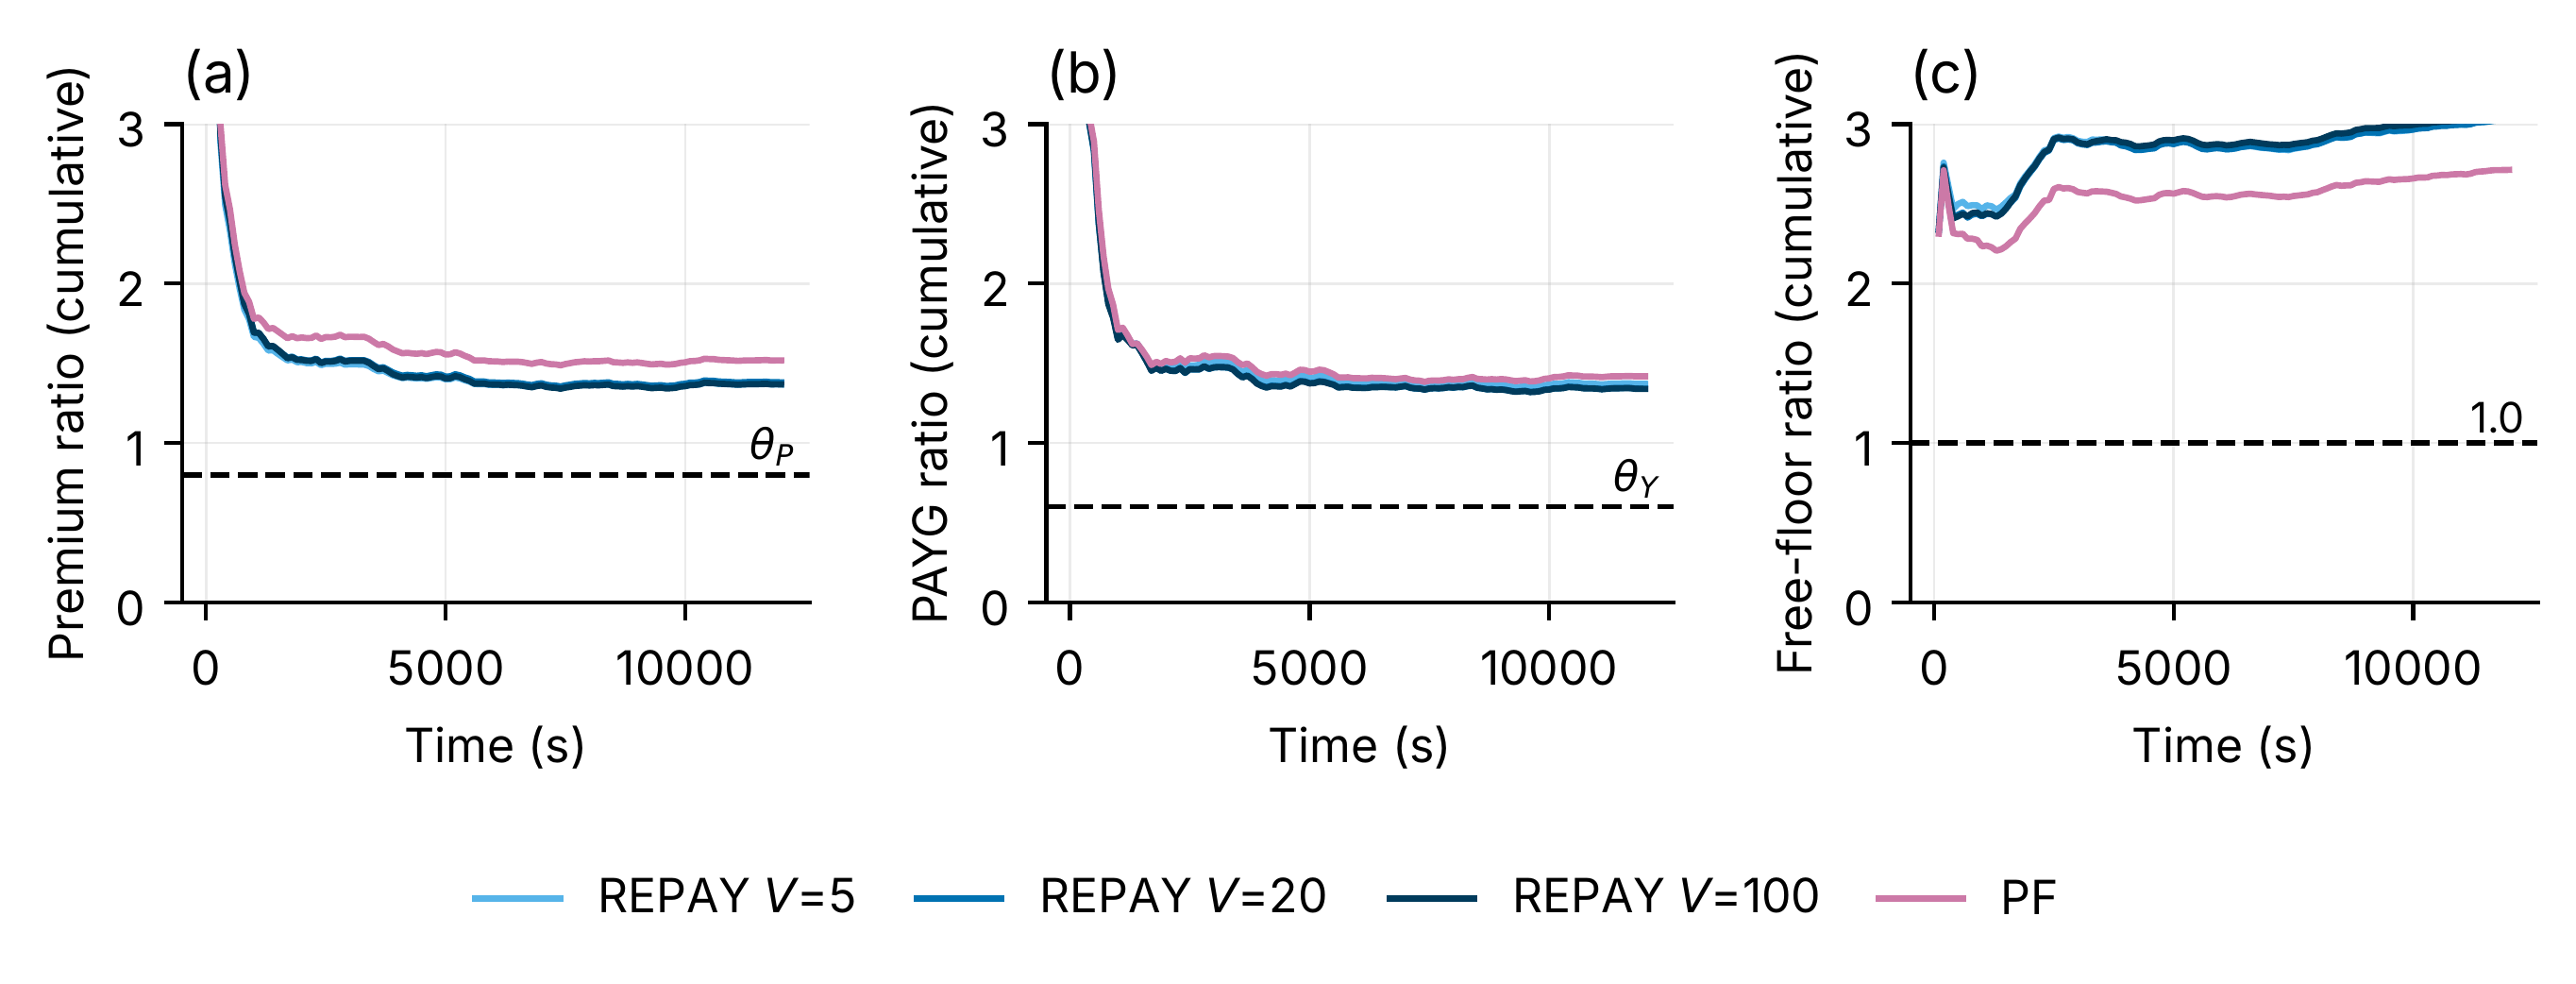
\includegraphics[width=\linewidth]{fig_tiers.png}
\caption{Running averages of the three service levels relative to their targets (dashed), default configuration.}
\label{fig:tiers}
\end{figure}

\begin{table}[t]
\centering
\caption{Equal tier weights and demanding targets: the business constraints bind (mean over 5 seeds $\pm$ half-width of the 95\% confidence interval).}
\label{tab:tiers-binding}
\resizebox{0.9\linewidth}{!}{\begin{tabular}{lcccccc}
\toprule
Mechanism & Premium ($\ge 0.8$) & PAYG ($\ge 0.7$) & Free-floor ($\ge 1.0$) & Utility & RT success (\%) & Max envy (Mbit) \\
\midrule
REPAY & $0.819\pm0.012$ & $0.852\pm0.041$ & $2.434\pm0.081$ & $72.89\pm5.68$ & $94.5\pm2.0$ & $16.48\pm1.72$ \\
Plain DPP & $0.821\pm0.013$ & $0.859\pm0.039$ & $2.425\pm0.083$ & $75.23\pm5.68$ & $99.5\pm0.6$ & $1038.51\pm111.09$ \\
PF & $0.549\pm0.023$ & $0.833\pm0.044$ & $3.041\pm0.092$ & $72.61\pm5.24$ & $88.5\pm1.7$ & $0.00\pm0.00$ \\
WFQ & $0.550\pm0.019$ & $0.833\pm0.057$ & $3.038\pm0.089$ & $76.78\pm5.24$ & $100.0\pm0.0$ & $1825.24\pm103.67$ \\
Priority & $0.550\pm0.019$ & $0.833\pm0.057$ & $3.038\pm0.089$ & $76.78\pm5.24$ & $100.0\pm0.0$ & $1825.24\pm103.67$ \\
Credit & $0.551\pm0.028$ & $0.828\pm0.036$ & $3.042\pm0.089$ & $64.58\pm5.34$ & $77.6\pm3.8$ & $120.67\pm46.98$ \\
\bottomrule
\end{tabular}}
\end{table}

\subsection{Running time}\label{sec:exp-runtime}

The solver performs at most $80$ bisection steps per slot, each a vectorised pass over the devices.
On single-slot instances with $10$ to $3000$ devices the median solve time stays between $1.4$ and $2.0$~ms on one core of a commodity server (Figure~\ref{fig:runtime}); a conic solver applied to the same problem takes $11$ to $27$~ms for $10$ to $300$ devices and agrees with the bisection to a relative difference of $10^{-8}$ in the objective (evaluated at the conic solver's primal point).
The complete allocation step, including rounding and bookkeeping, takes about $1.5$~ms per slot on average in the hotspot scenario (about $75$ devices) in our simulator, so one-second slots leave more than two orders of magnitude of headroom.

\begin{figure}[t]
\centering
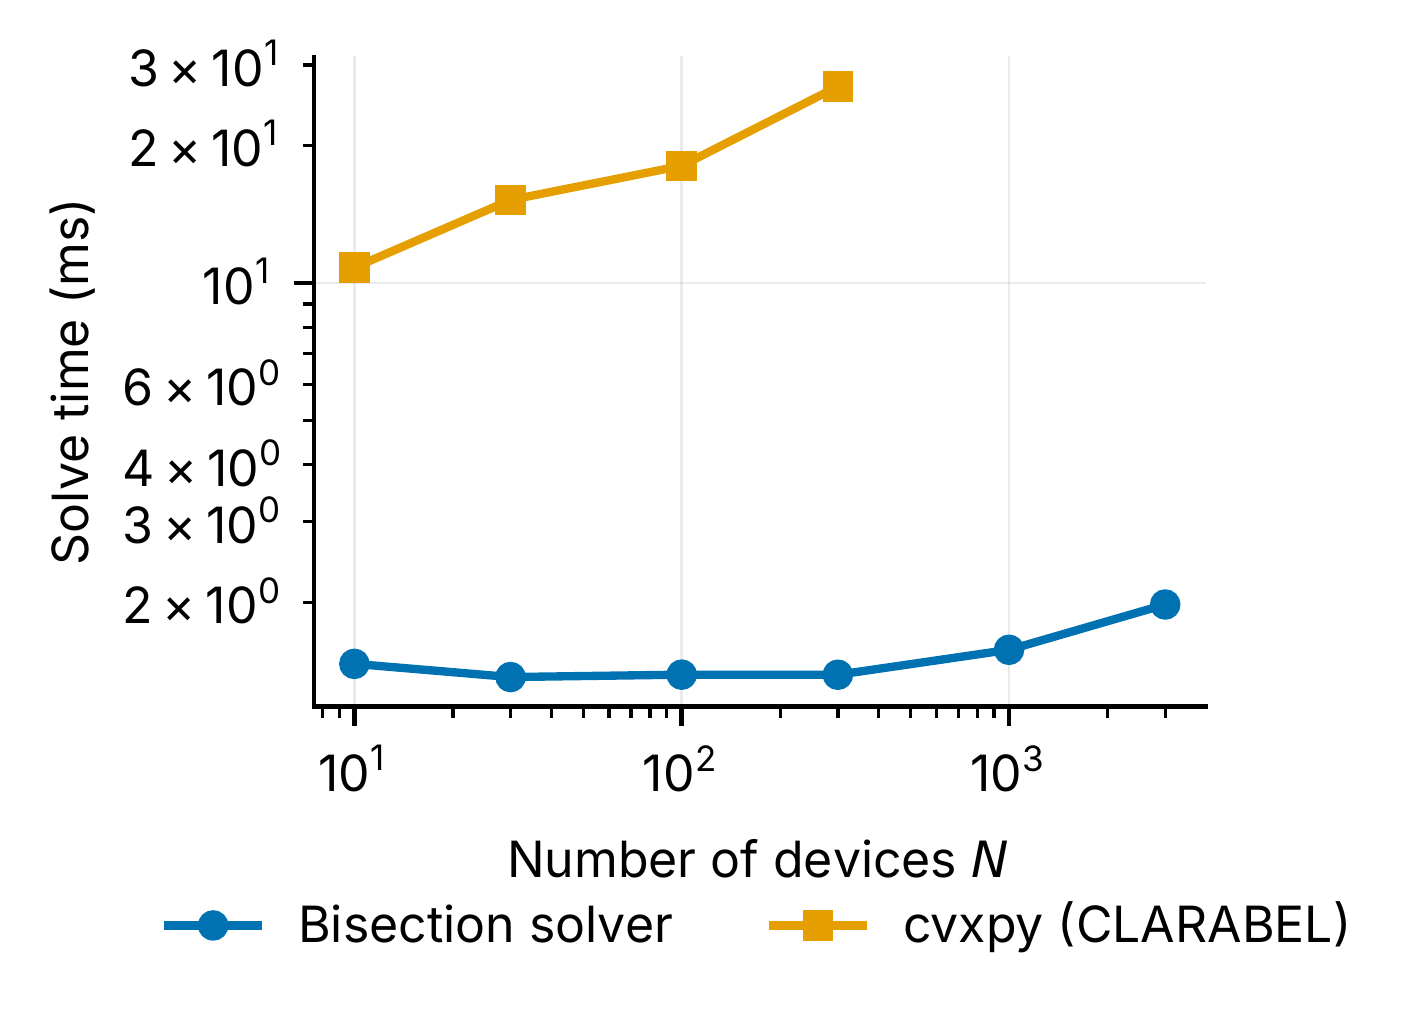
\includegraphics[width=0.45\linewidth]{fig_runtime.png}
\caption{Time to solve one slot against the number of active devices.}
\label{fig:runtime}
\end{figure}


\section{Discussion and limitations}\label{sec:discussion}

\paragraph{What bounded envy costs.}
Class-envy-freeness ties the volume of a real-time flow to that of its elastic tier-mates.
When capacity per device stays below $\rmin_k$ for a long time, no rule can serve every call without making calls permanently better off than downloads, and \repay{} then admits calls part of the time.
We conjecture, without proof, that an operator who prefers to protect calls in such regimes can scale the reference by a factor $\gamma<1$, at the price of an incentive slack proportional to $1-\gamma$, or sell the protection: a premium tier with a larger weight $w_g$ has a larger envy bound and therefore a longer horizon over which its calls can borrow.

\paragraph{The size of the bound.}
The bound grows linearly in $V$ and the utility gap shrinks as $1/V$.
For a device that stays $L$ slots the incentive to misreport is at most $B/L$ per slot, so short visits are weakly protected, and a device that leaves before it is repaid keeps its loss; this is hard to avoid for a rule that settles accounts over time. At $V=20$ the video bound is a sixth to a little over a quarter of the volume of a median stay (Table~\ref{tab:bsize}), and among devices that stay less than a minute almost nine in ten gain by misreporting, by a median of $12\%$ (Table~\ref{tab:short}).
The gaming class has a small rate, hence a large $\eta_{\mathrm{g}}$ and a loose $B_{g,\mathrm{g}}$, although the envy it can actually cause is small because its rate is small.

\paragraph{Incentives.}
Our guarantees are of three kinds, and they should not be confused.
The envy bound is exact and holds on every path; technically it is a deterministic queue bound of the kind familiar from drift-plus-penalty analysis, and what is specific to our construction is that the queue measures the envy of one device and that the tier prices cancel.
The translation into incentives assumes price-taking devices; it is an approximation that fails in thin tiers and degrades over long stays: in the trace-driven scenario $9$ devices in $120$ gained more than the bound, eight of them by up to a factor $1.8$ and one, often the only video flow of a premium tier with $25$ devices, by a factor of twelve, and in a second trace-driven scenario five devices gained up to $2.2$ times the bound. On the synthetic hotspot no device of the $180$ exceeded it, but the largest gain reached three quarters of it. The experiments, not the theorem, are the evidence on incentives.
Finally, the approach relies on two operational assumptions: demand is measured by the access point, which holds for downlink traffic, and a subscriber cannot change its declared class more often than every $\tau$ slots.
Uplink demand would have to be inferred from buffer reports, which a device can inflate; the credit held at any time through such inflation is at most one envy bound, but we did not bound repeated accumulation, nor model its cost to others.
Most of the empirical incentive effect is already present when only the bonus of the elastic device is kept and the debt price of the RT group is dropped (variant No-debt: median change $+1.5\%$ against $+1.3\%$, $66\%$ of devices gaining against $63\%$), although the mean relative gain is then $+10\%$ instead of $-0.1\%$; in the synthetic experiments the debt price also lowers envy, from $25$ to $15$~Mbit, at a cost of $2.6$ points of RT success.
The simple monotonicity one would like for dynamic strategies fails, so for switching strategies our analytical statement covers only the phases in which the device poses as real-time.
The rotation that equalises admissions inside a real-time group, which the incentive argument needs, had no measurable effect on call continuity in our experiments (Table~\ref{tab:continuity}).

\paragraph{Modelling choices.}
We treat a single bottleneck with slot-level rates.
Latency inside a slot, which matters for gaming, is represented only through the requirement of service in every slot.
Several access points that share a backhaul would add a second layer of capacity constraints; the per-slot problem remains concave, but the bisection on one price would become a small dual problem.
The utility theorem assumes that the population process and the demand caps do not react to the allocation, whereas real users leave when service is poor and finite transfers end sooner when served faster; its benchmark imposes the business constraints in every population state, and its constant is too large for the bound to be informative at the parameter values we simulate.
The business constraints are stated per unit of rate; a commitment on the admission probability of premium calls would break the cancellation used in Theorem~\ref{thm:bound} and add the corresponding multiplier to the bound.
The evaluation is by simulation at the level of one-second rates. Most of it uses synthetic traces; the trace-driven experiments take arrivals, stays and demand levels from public Wi-Fi session logs and capacity from mobile throughput logs, but classes are inferred from session averages by a heuristic, tiers are drawn from a rough estimate, the two sources are unrelated to each other, and the session logs give a mean rate per session, not a demand process; capacity is an exogenous number of Mbit/s, not airtime shared by stations with different physical rates; every device keeps one class for its stay; elastic devices are saturated while active, so we did not test finite transfers, for which later repayment is worth less; and several experiments use two to five traces. The two further trace-driven scenarios are weaker still: very light elastic demand, short stays, a whole network pooled into one link in one case, counters of doubtful direction in the other, and data whose licences are not stated. A packet-level implementation on an access point, with real applications, is the natural next step, and without it the results say how the allocation rule behaves, not how calls would sound.
In the simulations a simpler rule, strict priority with a cap on the share of capacity given to RT flows, protects about as many RT slots as \repay{} at a higher elastic rate when its cap suits the traffic mix (Figure~\ref{fig:frontier}); with fewer real-time devices the same cap stops binding and rewards misreporting nearly as much as strict priority does (Section~\ref{sec:exp-mix}). In the trace-driven scenario, where real-time traffic is rarer, the same cap and the plain priority rules all serve many more RT slots than \repay{}; the cap does so at about the same elastic rate, while plain priority and \textsc{WFQ} lower it by $27$--$28\%$ and plain DPP by $11\%$ (Section~\ref{sec:exp-real}), and raising $V$ does not close the gap. What does help there is to drop the debt price and lower $V$: at $V=5$ the variant without the debt price serves about six points more RT slots than the full rule at $V=20$ with less than half the envy, a similar, negligible, median gain from misreporting, and fewer devices above the bound. At larger $V$ the variant leaves a growing incentive to misreport (a median gain of $20\%$ at $V=200$), and on one of the two further trace-driven scenarios the same low-$V$ variant is the more manipulable configuration, with $13$ of $120$ devices above its smaller bound against five under the default. Our default, chosen on synthetic traces where the two variants differed by under three points, is thus not the best configuration on the Paris traces, and we report both. Among six further baselines adapted from the literature, those that serve more RT slots than \repay{} reward misreporting and the others serve fewer. What \repay{} adds is the bound for every elastic device, the independence of that bound from the traffic mix, and the business constraints; an operator who needs none of these and knows its traffic mix may prefer the cap.
Calls are interrupted under \repay{} more often than under the priority rules and plain DPP, in $7.6\%$ of their slots (Table~\ref{tab:continuity}), since nothing in the objective penalises an interruption.
The comparisons use fixed values of $V$, of the tier weights and of the capacity level, chosen before the comparison runs and not tuned afterwards; with these values the business constraints are slack, and they bind only in the dedicated experiment of Section~\ref{sec:exp-tiers}.
The gain from misreporting is measured for a video bundle capped at $3$~Mbit/s, a cap that by itself makes the deviation unattractive to devices with a large fair share; the credit baseline and the six additional baselines are our adaptations of published systems and mechanisms, not those systems.

\section{Conclusion}\label{sec:conclusion}

Protecting real-time traffic on a shared access link invites every other application to claim to be real-time.
We proposed to grant the protection on credit: priority now is paid back in volume later, through per-device deficit queues embedded in a drift-plus-penalty allocation with commercial tiers and long-run business constraints.
The resulting rule bounds the envy between service classes by a constant on every sample path and for every device, whatever the churn, while its fluid allocation stays within $O(1/V)$, in utility, of a benchmark of policies that meet the business constraints and are class-envy-free in expectation in every population state.
It is not the rule with the best averages: a capped strict priority tuned to the traffic mix can serve as many real-time slots at a higher elastic rate, and when real-time traffic is rare plain priority serves more of it ($15$ points more on the Paris traces, $3$ to $8$ on the two further scenarios); on synthetic traces \repay{} serves $95\%$ of real-time slots against $82\%$ for proportional fairness at a similar elastic rate, and it is the choice when each delay-tolerant user must be guaranteed what it is owed.
The construction is not tied to access networks.
It applies wherever an operator must differentiate users whose needs differ in timing rather than in quantity and cannot verify what they are, for instance in shared compute clusters with interactive and batch jobs or in charging infrastructure; adapting the analysis to several resources and to learned, rather than declared, classes are the directions we find most interesting.


\section*{Declaration of competing interest}
The author declares that he has no known competing financial interests or personal relationships that could have appeared to influence the work reported in this paper.

\section*{Data availability}
All code, random seeds and result files needed to reproduce the figures and tables are available at \url{https://github.com/vinhqdang/computer_network_optimization}. The public datasets used in Section~\ref{sec:exp-real} and the subsequent trace-driven scenarios are available from their publishers under the licences stated in the repository.

\section*{CRediT authorship contribution statement}
\textbf{Quang-Vinh Dang}: Conceptualization, Methodology, Software, Validation, Formal analysis, Investigation, Data curation, Writing -- original draft, Writing -- review \& editing, Visualization.

\appendix
\section{Proofs}\label{app:proofs}

\subsection{Proof of Proposition~\ref{prop:reverse}}\label{app:reverse}

Fix a slot and a tier $g$ whose deficits are all zero, so that $\pi_{g,k}=\zeta_{g,k}=0$ and elastic devices of the tier have no bonus.
The flow takes $\lambda$, $\beta_g$, the size of its group and the group's offer as given, and we compare with the fluid elastic allocation (the leftover that rounding may add to an elastic device is ignored).
Write $\lambda'=\lambda-\beta_g$ and $w=w_g$.
A class-$k$ flow that declared $E$ would receive at most $\hat x$, where $\hat x$ is the unconstrained elastic response: $\hat x=\infty$ if $\lambda'\le0$ and $Vw\,u'(\hat x)=\lambda'$ otherwise (with $\hat x=0$ if $\lambda'\ge Vw\,u'(0)$).
Its true utility from a rate $x$ is $\tilde u_k(x)=u_k(\min(x,\rmax_k))\,\ind\{x\ge\rmin_k\}$, which is nondecreasing, so it suffices to show that the offer of group $(g,k)$ is worth at least $\tilde u_k(\hat x)$.

If $\hat x<\rmin_k$ then $\tilde u_k(\hat x)=0$ and there is nothing to prove.
Otherwise put $\bar x=\min(\hat x,\rmax_k)\ge\rmin_k$.
Since $u'$ is decreasing, $\lambda'\le Vw\,u'(\hat x)\le Vw\,u'(\bar x)\le Vw\,u'(\rmin_k)$.

\emph{Rate.} With zero debts, $\psi_{g,k}(z;\lambda)=n[Vw\,u_k(z)-\lambda'z]$. For $z\le\bar x$, concavity of $u_k$ and the first hypothesis give $Vw\,u_k'(z)\ge Vw\,u_k'(\bar x)\ge Vw\,u'(\bar x)\ge\lambda'$, so $\psi$ is nondecreasing on $[\rmin_k,\bar x]$ and $z^*\ge\bar x$. (If $\rmin_k=\rmax_k$ then $z^*=\bar x$ trivially.)

\emph{Admission.} By the second hypothesis, $\max_z\psi\ge\psi(\rmin_k)=n[Vw\,u_k(\rmin_k)-\lambda'\rmin_k]\allowbreak>n\,\rmin_k[Vw\,u'(\rmin_k)-\lambda']\ge0$, so $a^*=1$.

Hence the flow is admitted at rate $z^*\ge\bar x$ and its utility is $u_k(z^*)\ge u_k(\bar x)=\tilde u_k(\hat x)$.

For $u(x)=\log(1+x)$ and $u_{\mathrm{v}}(z)=1+\log(z/\rmin_{\mathrm{v}})$ the hypotheses read $1/z\ge1/(1+z)$ and $1>\rmin_{\mathrm{v}}/(1+\rmin_{\mathrm{v}})$; for gaming, $1>r_{\mathrm{g}}/(1+r_{\mathrm{g}})$. \qed

\subsection{Proof of Theorem~\ref{thm:opt}}\label{app:opt}

Let $\Phi(t)=\tfrac12\sum_jQ_j(t)^2+\tfrac12\sum_{i\in\cE_t}\sum_{k\in\cK}D_{i,k}(t)^2$.

\emph{One-slot drift.}
From \eqref{eq:Q}, $Q_j(t+1)^2\le(Q_j(t)+e_{j,t})^2$, so
$\tfrac12Q_j(t+1)^2-\tfrac12Q_j(t)^2\le Q_j(t)e_{j,t}+\tfrac12(e_j^{\max})^2$.
From \eqref{eq:D}, in the same way and using $|r_{i,k,t}-x_{i,t}|\le\ell^{\max}$, $D_{i,k}(t)\ge0$ and $r_{i,k,t}\le a\,m_{d_{i,t}}(z)$,
\[
\tfrac12D_{i,k}(t+1)^2-\tfrac12D_{i,k}(t)^2\le D_{i,k}(t)\big(a_{g_i,k}\,m_{d_{i,t}}(z_{g_i,k})-x_{i,t}\big)+\tfrac12(\ell^{\max})^2 .
\]
Between slots $t$ and $t+1$ the population changes. A device that leaves removes the nonnegative term $\tfrac12\sum_kD_{i,k}^2$ from $\Phi$, and a device that arrives contributes zero. Summing over the at most $N_{\max}$ elastic devices of slot $t$,
\[
\Phi(t+1)-\Phi(t)\le B_0+\sum_jQ_j(t)e_{j,t}+\sum_{i\in\cE_t}\sum_kD_{i,k}(t)\big(a\,m_{d_{i,t}}(z)-x_{i,t}\big).
\]
Subtracting $VU_t$ from both sides, the right-hand side becomes $B_0$ minus the expression \eqref{eq:dpp}, which is the objective of \eqref{eq:slot} up to a decision-independent constant. \repay{} maximises that objective over all feasible decisions, and a policy $\mu\in\Pi(\xi_t)$ returns, for the realised $C_t$, a feasible decision of the same problem, so
\begin{equation}\label{eq:app1}\begin{aligned}
\Phi(t+1)-\Phi(t)-VU_t&\le B_0+\sum_jQ_j(t)e^{\mu}_{j,t}\\&\quad+\sum_{i,k}D_{i,k}(t)\big(a^\mu m_{d_{i,t}}(z^\mu)-x^\mu_{i}\big)-VU^{\mu}_t .
\end{aligned}\end{equation}

\emph{Comparison with the benchmark.}
Let $\mathcal H_t$ consist of the history up to the start of slot $t$ together with $\xi_t$; the queues $Q(t)$ and $D(t)$ are $\mathcal H_t$-measurable.
By Assumption~\ref{ass:model}(ii), $C_t$ has distribution $F_{\xi_t}$ conditionally on $\mathcal H_t$, and $\mu$ depends on $C_t$ only (and on independent randomisation).
Taking conditional expectations in \eqref{eq:app1} and using \eqref{eq:bench},
\[
\E\big[\Phi(t+1)-\Phi(t)-VU_t\mid\mathcal H_t\big]\le B_0-V\,\E_{F_{\xi_t}}[U(\mu)],
\]
because the queues are nonnegative and multiply quantities with nonpositive conditional mean.
Letting $\mu$ approach the supremum, the right-hand side becomes $B_0-VU^*(\xi_t)$.

\emph{Telescoping.}
Take expectations, sum over $t=1,\dots,T$, and use $\Phi(1)=0$, $\Phi(T+1)\ge0$:
\[
-V\sum_{t\le T}\E[U_t]\le TB_0-V\sum_{t\le T}\E[U^*(\xi_t)],
\]
which is the utility bound after dividing by $VT$.
The same inequality with $U^*\ge0$ and $U_t\le U^{\max}$ gives $\E[\Phi(T+1)]\le T(B_0+VU^{\max})$.
Since $Q_j(T+1)\ge\sum_{t\le T}e_{j,t}$ by \eqref{eq:Q} and $\E[Q_j(T+1)]\le\sqrt{\E[Q_j(T+1)^2]}\le\sqrt{2\,\E[\Phi(T+1)]}$,
\[
\frac1T\sum_{t\le T}\E[e_{j,t}]\le\frac{\E[Q_j(T+1)]}{T}\le\sqrt{\frac{2(B_0+VU^{\max})}{T}} .
\]

\emph{Sample paths.}
The previous step also gives $\E[(Q_j(T+1)/T)^2]\le2(B_0+VU^{\max})/T$.
Along $T=m^2$ these bounds are summable, so by Chebyshev's inequality and the Borel--Cantelli lemma $Q_j(m^2+1)/m^2\to0$ almost surely.
For $m^2\le T<(m+1)^2$ the increments of $Q_j$ are bounded by $e_j^{\max}$, hence $Q_j(T+1)\le Q_j(m^2+1)+(2m+1)e_j^{\max}$ and $Q_j(T+1)/T\to0$ almost surely.
As $\sum_{t\le T}e_{j,t}\le Q_j(T+1)$, the long-run averages in \eqref{eq:ps}--\eqref{eq:ff} are nonpositive on almost every path. \qed


\begin{thebibliography}{99}
\expandafter\ifx\csname natexlab\endcsname\relax\def\natexlab#1{#1}\fi
\providecommand{\url}[1]{\texttt{#1}}
\providecommand{\href}[2]{#2}
\providecommand{\path}[1]{#1}
\providecommand{\DOIprefix}{doi:}
\providecommand{\ArXivprefix}{arXiv:}
\providecommand{\URLprefix}{URL: }
\providecommand{\Pubmedprefix}{pmid:}
\providecommand{\doi}[1]{\href{http://dx.doi.org/#1}{\path{#1}}}
\providecommand{\Pubmed}[1]{\href{pmid:#1}{\path{#1}}}
\providecommand{\bibinfo}[2]{#2}
\ifx\xfnm\relax \def\xfnm[#1]{\unskip,\space#1}\fi
%Type = Article
\bibitem[{Kelly et~al.(1998)Kelly, Maulloo, and Tan}]{kelly1998rate}
\bibinfo{author}{F.~P. Kelly}, \bibinfo{author}{A.~K. Maulloo},
  \bibinfo{author}{D.~K.~H. Tan},
\newblock \bibinfo{title}{Rate control for communication networks: shadow
  prices, proportional fairness and stability},
\newblock \bibinfo{journal}{Journal of the Operational Research Society}
  \bibinfo{volume}{49} (\bibinfo{year}{1998}) \bibinfo{pages}{237--252}.
  \DOIprefix\doi{10.1057/palgrave.jors.2600523}.
%Type = Article
\bibitem[{Mo and Walrand(2000)}]{mo2000fair}
\bibinfo{author}{J.~Mo}, \bibinfo{author}{J.~Walrand},
\newblock \bibinfo{title}{Fair end-to-end window-based congestion control},
\newblock \bibinfo{journal}{IEEE/ACM Transactions on Networking}
  \bibinfo{volume}{8} (\bibinfo{year}{2000}) \bibinfo{pages}{556--567}.
  \DOIprefix\doi{10.1109/90.879343}.
%Type = Inproceedings
\bibitem[{Lan et~al.(2010)Lan, Kao, Chiang, and Sabharwal}]{lan2010axiomatic}
\bibinfo{author}{T.~Lan}, \bibinfo{author}{D.~Kao},
  \bibinfo{author}{M.~Chiang}, \bibinfo{author}{A.~Sabharwal},
\newblock \bibinfo{title}{An axiomatic theory of fairness in network resource
  allocation},
\newblock in: \bibinfo{booktitle}{Proc. IEEE INFOCOM}, \bibinfo{year}{2010},
  pp. \bibinfo{pages}{1--9}. \DOIprefix\doi{10.1109/INFCOM.2010.5461911}.
  \href{http://arxiv.org/abs/0906.0557}{{\tt arXiv:0906.0557}}.
%Type = Article
\bibitem[{Bertsimas et~al.(2011)Bertsimas, Farias, and
  Trichakis}]{bertsimas2011price}
\bibinfo{author}{D.~Bertsimas}, \bibinfo{author}{V.~F. Farias},
  \bibinfo{author}{N.~Trichakis},
\newblock \bibinfo{title}{The price of fairness},
\newblock \bibinfo{journal}{Operations Research} \bibinfo{volume}{59}
  (\bibinfo{year}{2011}) \bibinfo{pages}{17--31}.
  \DOIprefix\doi{10.1287/opre.1100.0865}.
%Type = Article
\bibitem[{Shenker(1995)}]{shenker1995fundamental}
\bibinfo{author}{S.~Shenker},
\newblock \bibinfo{title}{Fundamental design issues for the future {Internet}},
\newblock \bibinfo{journal}{IEEE Journal on Selected Areas in Communications}
  \bibinfo{volume}{13} (\bibinfo{year}{1995}) \bibinfo{pages}{1176--1188}.
  \DOIprefix\doi{10.1109/49.414637}.
%Type = Article
\bibitem[{Lee et~al.(2005)Lee, Mazumdar, and Shroff}]{lee2005nonconvex}
\bibinfo{author}{J.-W. Lee}, \bibinfo{author}{R.~R. Mazumdar},
  \bibinfo{author}{N.~B. Shroff},
\newblock \bibinfo{title}{Non-convex optimization and rate control for
  multi-class services in the {Internet}},
\newblock \bibinfo{journal}{IEEE/ACM Transactions on Networking}
  \bibinfo{volume}{13} (\bibinfo{year}{2005}) \bibinfo{pages}{827--840}.
  \DOIprefix\doi{10.1109/TNET.2005.852876}.
%Type = Article
\bibitem[{Hande et~al.(2007)Hande, Zhang, and Chiang}]{hande2007distributed}
\bibinfo{author}{P.~Hande}, \bibinfo{author}{S.~Zhang},
  \bibinfo{author}{M.~Chiang},
\newblock \bibinfo{title}{Distributed rate allocation for inelastic flows},
\newblock \bibinfo{journal}{IEEE/ACM Transactions on Networking}
  \bibinfo{volume}{15} (\bibinfo{year}{2007}) \bibinfo{pages}{1240--1253}.
  \DOIprefix\doi{10.1109/TNET.2007.896507}.
%Type = Article
\bibitem[{Parekh and Gallager(1993)}]{parekh1993generalized}
\bibinfo{author}{A.~K. Parekh}, \bibinfo{author}{R.~G. Gallager},
\newblock \bibinfo{title}{A generalized processor sharing approach to flow
  control in integrated services networks: the single-node case},
\newblock \bibinfo{journal}{IEEE/ACM Transactions on Networking}
  \bibinfo{volume}{1} (\bibinfo{year}{1993}) \bibinfo{pages}{344--357}.
  \DOIprefix\doi{10.1109/90.234856}.
%Type = Article
\bibitem[{Shreedhar and Varghese(1996)}]{shreedhar1996efficient}
\bibinfo{author}{M.~Shreedhar}, \bibinfo{author}{G.~Varghese},
\newblock \bibinfo{title}{Efficient fair queuing using deficit round-robin},
\newblock \bibinfo{journal}{IEEE/ACM Transactions on Networking}
  \bibinfo{volume}{4} (\bibinfo{year}{1996}) \bibinfo{pages}{375--385}.
  \DOIprefix\doi{10.1109/90.502236}.
%Type = Misc
\bibitem[{H{\o}iland-J{\o}rgensen et~al.(2017)H{\o}iland-J{\o}rgensen, Kazior,
  T{\"a}ht, Hurtig, and Brunstrom}]{hoiland2017ending}
\bibinfo{author}{T.~H{\o}iland-J{\o}rgensen}, \bibinfo{author}{M.~Kazior},
  \bibinfo{author}{D.~T{\"a}ht}, \bibinfo{author}{P.~Hurtig},
  \bibinfo{author}{A.~Brunstrom}, \bibinfo{title}{Ending the anomaly: Achieving
  low latency and airtime fairness in {WiFi}}, \bibinfo{year}{2017}.
  \href{http://arxiv.org/abs/1703.00064}{{\tt arXiv:1703.00064}}.
%Type = Article
\bibitem[{Si~Salem et~al.(2022)Si~Salem, Iosifidis, and
  Neglia}]{sisalem2023enabling}
\bibinfo{author}{T.~Si~Salem}, \bibinfo{author}{G.~Iosifidis},
  \bibinfo{author}{G.~Neglia},
\newblock \bibinfo{title}{Enabling long-term fairness in dynamic resource
  allocation},
\newblock \bibinfo{journal}{Proc. ACM Meas. Anal. Comput. Syst.}
  \bibinfo{volume}{6} (\bibinfo{year}{2022}) \bibinfo{pages}{1--36}.
  \DOIprefix\doi{10.1145/3570606}. \href{http://arxiv.org/abs/2208.05898}{{\tt
  arXiv:2208.05898}}.
%Type = Inproceedings
\bibitem[{ElAzzouni et~al.(2020)ElAzzouni, Ekici, and
  Shroff}]{elazzouni2020deadline}
\bibinfo{author}{S.~ElAzzouni}, \bibinfo{author}{E.~Ekici},
  \bibinfo{author}{N.~Shroff},
\newblock \bibinfo{title}{Is deadline oblivious scheduling efficient for
  controlling real-time traffic in cellular downlink systems?},
\newblock in: \bibinfo{booktitle}{Proc. IEEE INFOCOM}, \bibinfo{year}{2020},
  pp. \bibinfo{pages}{49--58}.
  \DOIprefix\doi{10.1109/INFOCOM41043.2020.9155523}.
  \href{http://arxiv.org/abs/2002.06474}{{\tt arXiv:2002.06474}}.
%Type = Techreport
\bibitem[{Szigeti et~al.(2018)Szigeti, Henry, and Baker}]{rfc8325}
\bibinfo{author}{T.~Szigeti}, \bibinfo{author}{J.~Henry},
  \bibinfo{author}{F.~Baker}, \bibinfo{title}{Mapping {Diffserv} to {IEEE}
  802.11}, \bibinfo{type}{RFC} \bibinfo{number}{8325}, Internet Engineering
  Task Force, \bibinfo{year}{2018}. \DOIprefix\doi{10.17487/RFC8325}.
%Type = Article
\bibitem[{Rezaei and Liu(2019)}]{rezaei2019deep}
\bibinfo{author}{S.~Rezaei}, \bibinfo{author}{X.~Liu},
\newblock \bibinfo{title}{Deep learning for encrypted traffic classification:
  An overview},
\newblock \bibinfo{journal}{IEEE Communications Magazine} \bibinfo{volume}{57}
  (\bibinfo{year}{2019}) \bibinfo{pages}{76--81}.
  \DOIprefix\doi{10.1109/MCOM.2019.1800819}.
%Type = Techreport
\bibitem[{H{\o}iland-J{\o}rgensen
  et~al.(2018{\natexlab{a}})H{\o}iland-J{\o}rgensen, McKenney, T{\"a}ht,
  Gettys, and Dumazet}]{rfc8290}
\bibinfo{author}{T.~H{\o}iland-J{\o}rgensen}, \bibinfo{author}{P.~McKenney},
  \bibinfo{author}{D.~T{\"a}ht}, \bibinfo{author}{J.~Gettys},
  \bibinfo{author}{E.~Dumazet}, \bibinfo{title}{The Flow Queue {CoDel} Packet
  Scheduler and Active Queue Management Algorithm}, \bibinfo{type}{RFC}
  \bibinfo{number}{8290}, Internet Engineering Task Force,
  \bibinfo{year}{2018}{\natexlab{a}}. \DOIprefix\doi{10.17487/RFC8290}.
%Type = Inproceedings
\bibitem[{H{\o}iland-J{\o}rgensen
  et~al.(2018{\natexlab{b}})H{\o}iland-J{\o}rgensen, T{\"a}ht, and
  Morton}]{hoiland2018cake}
\bibinfo{author}{T.~H{\o}iland-J{\o}rgensen}, \bibinfo{author}{D.~T{\"a}ht},
  \bibinfo{author}{J.~Morton},
\newblock \bibinfo{title}{Piece of {CAKE}: A comprehensive queue management
  solution for home gateways},
\newblock in: \bibinfo{booktitle}{IEEE International Symposium on Local and
  Metropolitan Area Networks (LANMAN)}, \bibinfo{year}{2018}{\natexlab{b}}, pp.
  \bibinfo{pages}{37--42}. \DOIprefix\doi{10.1109/LANMAN.2018.8475045}.
%Type = Techreport
\bibitem[{Briscoe et~al.(2023)Briscoe, De~Schepper, Bagnulo, and
  White}]{rfc9330}
\bibinfo{author}{B.~Briscoe}, \bibinfo{author}{K.~De~Schepper},
  \bibinfo{author}{M.~Bagnulo}, \bibinfo{author}{G.~White}, \bibinfo{title}{Low
  Latency, Low Loss, and Scalable Throughput ({L4S}) {Internet} Service:
  Architecture}, \bibinfo{type}{RFC} \bibinfo{number}{9330}, Internet
  Engineering Task Force, \bibinfo{year}{2023}.
  \DOIprefix\doi{10.17487/RFC9330}.
%Type = Article
\bibitem[{Georgiadis et~al.(2006)Georgiadis, Neely, and
  Tassiulas}]{georgiadis2006resource}
\bibinfo{author}{L.~Georgiadis}, \bibinfo{author}{M.~J. Neely},
  \bibinfo{author}{L.~Tassiulas},
\newblock \bibinfo{title}{Resource allocation and cross-layer control in
  wireless networks},
\newblock \bibinfo{journal}{Foundations and Trends in Networking}
  \bibinfo{volume}{1} (\bibinfo{year}{2006}) \bibinfo{pages}{1--144}.
  \DOIprefix\doi{10.1561/1300000001}.
%Type = Book
\bibitem[{Neely(2010)}]{neely2010stochastic}
\bibinfo{author}{M.~J. Neely}, \bibinfo{title}{Stochastic Network Optimization
  with Application to Communication and Queueing Systems}, Synthesis Lectures
  on Learning, Networks, and Algorithms, \bibinfo{publisher}{Morgan \&
  Claypool}, \bibinfo{year}{2010}. \DOIprefix\doi{10.1007/978-3-031-79995-2}.
%Type = Article
\bibitem[{Stolyar(2005)}]{stolyar2005maximizing}
\bibinfo{author}{A.~L. Stolyar},
\newblock \bibinfo{title}{Maximizing queueing network utility subject to
  stability: Greedy primal-dual algorithm},
\newblock \bibinfo{journal}{Queueing Systems} \bibinfo{volume}{50}
  (\bibinfo{year}{2005}) \bibinfo{pages}{401--457}.
  \DOIprefix\doi{10.1007/s11134-005-1450-0}.
%Type = Article
\bibitem[{Eryilmaz and Srikant(2007)}]{eryilmaz2007fair}
\bibinfo{author}{A.~Eryilmaz}, \bibinfo{author}{R.~Srikant},
\newblock \bibinfo{title}{Fair resource allocation in wireless networks using
  queue-length-based scheduling and congestion control},
\newblock \bibinfo{journal}{IEEE/ACM Transactions on Networking}
  \bibinfo{volume}{15} (\bibinfo{year}{2007}) \bibinfo{pages}{1333--1344}.
  \DOIprefix\doi{10.1109/TNET.2007.897944}.
%Type = Article
\bibitem[{Neely et~al.(2008)Neely, Modiano, and Li}]{neely2008fairness}
\bibinfo{author}{M.~J. Neely}, \bibinfo{author}{E.~Modiano},
  \bibinfo{author}{C.-P. Li},
\newblock \bibinfo{title}{Fairness and optimal stochastic control for
  heterogeneous networks},
\newblock \bibinfo{journal}{IEEE/ACM Transactions on Networking}
  \bibinfo{volume}{16} (\bibinfo{year}{2008}) \bibinfo{pages}{396--409}.
  \DOIprefix\doi{10.1109/TNET.2007.900405}.
%Type = Inproceedings
\bibitem[{Neely(2011)}]{neely2011worstcase}
\bibinfo{author}{M.~J. Neely},
\newblock \bibinfo{title}{Opportunistic scheduling with worst case delay
  guarantees in single and multi-hop networks},
\newblock in: \bibinfo{booktitle}{Proceedings IEEE INFOCOM},
  \bibinfo{year}{2011}, pp. \bibinfo{pages}{1728--1736}.
  \DOIprefix\doi{10.1109/INFCOM.2011.5934971}.
%Type = Article
\bibitem[{Jaramillo and Srikant(2011)}]{jaramillo2011elastic}
\bibinfo{author}{J.~J. Jaramillo}, \bibinfo{author}{R.~Srikant},
\newblock \bibinfo{title}{Optimal scheduling for fair resource allocation in ad
  hoc networks with elastic and inelastic traffic},
\newblock \bibinfo{journal}{IEEE/ACM Transactions on Networking}
  \bibinfo{volume}{19} (\bibinfo{year}{2011}) \bibinfo{pages}{1125--1136}.
  \DOIprefix\doi{10.1109/tnet.2010.2100083}.
%Type = Article
\bibitem[{Mahdavi et~al.(2012)Mahdavi, Jin, and Yang}]{mahdavi2012trading}
\bibinfo{author}{M.~Mahdavi}, \bibinfo{author}{R.~Jin},
  \bibinfo{author}{T.~Yang},
\newblock \bibinfo{title}{Trading regret for efficiency: Online convex
  optimization with long term constraints},
\newblock \bibinfo{journal}{Journal of Machine Learning Research}
  \bibinfo{volume}{13} (\bibinfo{year}{2012}) \bibinfo{pages}{2503--2528}.
  \href{http://arxiv.org/abs/1111.6082}{{\tt arXiv:1111.6082}}.
%Type = Inproceedings
\bibitem[{Yu et~al.(2017)Yu, Neely, and Wei}]{yu2017online}
\bibinfo{author}{H.~Yu}, \bibinfo{author}{M.~J. Neely},
  \bibinfo{author}{X.~Wei},
\newblock \bibinfo{title}{Online convex optimization with stochastic
  constraints},
\newblock in: \bibinfo{booktitle}{Advances in Neural Information Processing
  Systems}, volume~\bibinfo{volume}{30}, \bibinfo{year}{2017}.
  \href{http://arxiv.org/abs/1708.03741}{{\tt arXiv:1708.03741}}.
%Type = Article
\bibitem[{Yu and Neely(2020)}]{yu2019low}
\bibinfo{author}{H.~Yu}, \bibinfo{author}{M.~J. Neely},
\newblock \bibinfo{title}{A low complexity algorithm with {$O(\sqrt{T})$}
  regret and {$O(1)$} constraint violations for online convex optimization with
  long term constraints},
\newblock \bibinfo{journal}{Journal of Machine Learning Research}
  \bibinfo{volume}{21} (\bibinfo{year}{2020}) \bibinfo{pages}{1--24}.
  \href{http://arxiv.org/abs/1604.02218}{{\tt arXiv:1604.02218}}.
%Type = Article
\bibitem[{Balseiro et~al.(2023)Balseiro, Lu, and Mirrokni}]{balseiro2023best}
\bibinfo{author}{S.~R. Balseiro}, \bibinfo{author}{H.~Lu},
  \bibinfo{author}{V.~Mirrokni},
\newblock \bibinfo{title}{The best of many worlds: Dual mirror descent for
  online allocation problems},
\newblock \bibinfo{journal}{Operations Research} \bibinfo{volume}{71}
  (\bibinfo{year}{2023}) \bibinfo{pages}{101--119}.
  \DOIprefix\doi{10.1287/opre.2021.2242}.
  \href{http://arxiv.org/abs/2011.10124}{{\tt arXiv:2011.10124}}.
%Type = Article
\bibitem[{Balseiro et~al.(2025)Balseiro, Lu, and
  Mirrokni}]{balseiro2025regularized}
\bibinfo{author}{S.~R. Balseiro}, \bibinfo{author}{H.~Lu},
  \bibinfo{author}{V.~Mirrokni},
\newblock \bibinfo{title}{Regularized online allocation problems: Fairness and
  beyond},
\newblock \bibinfo{journal}{Manufacturing \& Service Operations Management}
  \bibinfo{volume}{27} (\bibinfo{year}{2025}) \bibinfo{pages}{720--735}.
  \DOIprefix\doi{10.1287/msom.2022.0212}.
  \href{http://arxiv.org/abs/2007.00514}{{\tt arXiv:2007.00514}}.
%Type = Misc
\bibitem[{Yu et~al.(2026)Yu, Lee, and Lee}]{yu2026slater}
\bibinfo{author}{K.~Yu}, \bibinfo{author}{J.~Lee}, \bibinfo{author}{D.~Lee},
  \bibinfo{title}{Constrained online convex optimization without slater's
  condition}, \bibinfo{year}{2026}. \href{http://arxiv.org/abs/2606.31480}{{\tt
  arXiv:2606.31480}}, \bibinfo{note}{arXiv preprint}.
%Type = Misc
\bibitem[{Sarkar and Sinha(2026)}]{sarkar2026geometric}
\bibinfo{author}{D.~Sarkar}, \bibinfo{author}{A.~Sinha}, \bibinfo{title}{A
  geometric approach to constrained online learning}, \bibinfo{year}{2026}.
  \href{http://arxiv.org/abs/2605.21107}{{\tt arXiv:2605.21107}},
  \bibinfo{note}{arXiv preprint (v3, Jul 2026)}.
%Type = Misc
\bibitem[{Abdullah et~al.(2026)Abdullah, Iosifidis, Elayoubi, and
  Chahed}]{abdullah2026dynamic}
\bibinfo{author}{M.~Abdullah}, \bibinfo{author}{G.~Iosifidis},
  \bibinfo{author}{S.~E. Elayoubi}, \bibinfo{author}{T.~Chahed},
  \bibinfo{title}{Dynamic optimistic constrained oco with memory via delay
  equivalence}, \bibinfo{year}{2026}.
  \href{http://arxiv.org/abs/2611.08302}{{\tt arXiv:2611.08302}},
  \bibinfo{note}{neurIPS 2026 (accepted, per arXiv comment)}.
%Type = Misc
\bibitem[{Sinclair et~al.(2021)Sinclair, Jain, Banerjee, and
  Yu}]{sinclair2021sequential}
\bibinfo{author}{S.~R. Sinclair}, \bibinfo{author}{G.~Jain},
  \bibinfo{author}{S.~Banerjee}, \bibinfo{author}{C.~L. Yu},
  \bibinfo{title}{Sequential fair allocation: Achieving the optimal
  envy-efficiency tradeoff curve}, \bibinfo{year}{2021}.
  \href{http://arxiv.org/abs/2105.05308}{{\tt arXiv:2105.05308}}.
%Type = Article
\bibitem[{Li et~al.(2020)Li, Liu, and Ji}]{li2020combinatorial}
\bibinfo{author}{F.~Li}, \bibinfo{author}{J.~Liu}, \bibinfo{author}{B.~Ji},
\newblock \bibinfo{title}{Combinatorial sleeping bandits with fairness
  constraints},
\newblock \bibinfo{journal}{IEEE Transactions on Network Science and
  Engineering} \bibinfo{volume}{7} (\bibinfo{year}{2020})
  \bibinfo{pages}{1799--1813}. \DOIprefix\doi{10.1109/TNSE.2019.2954310}.
  \href{http://arxiv.org/abs/1901.04891}{{\tt arXiv:1901.04891}}.
%Type = Article
\bibitem[{Mendelson and Whang(1990)}]{mendelson1990optimal}
\bibinfo{author}{H.~Mendelson}, \bibinfo{author}{S.~Whang},
\newblock \bibinfo{title}{Optimal incentive-compatible priority pricing for the
  {M/M/1} queue},
\newblock \bibinfo{journal}{Operations Research} \bibinfo{volume}{38}
  (\bibinfo{year}{1990}) \bibinfo{pages}{870--883}.
  \DOIprefix\doi{10.1287/opre.38.5.870}.
%Type = Article
\bibitem[{Af{\`e}che(2013)}]{afeche2013incentive}
\bibinfo{author}{P.~Af{\`e}che},
\newblock \bibinfo{title}{Incentive-compatible revenue management in queueing
  systems: Optimal strategic delay},
\newblock \bibinfo{journal}{Manufacturing \& Service Operations Management}
  \bibinfo{volume}{15} (\bibinfo{year}{2013}) \bibinfo{pages}{423--443}.
  \DOIprefix\doi{10.1287/msom.2013.0449}.
%Type = Inproceedings
\bibitem[{Odlyzko(1999)}]{odlyzko1999paris}
\bibinfo{author}{A.~Odlyzko},
\newblock \bibinfo{title}{Paris metro pricing for the {I}nternet},
\newblock in: \bibinfo{booktitle}{Proceedings of the 1st ACM Conference on
  Electronic Commerce}, \bibinfo{year}{1999}, pp. \bibinfo{pages}{140--147}.
  \DOIprefix\doi{10.1145/336992.337030}.
%Type = Article
\bibitem[{Sen et~al.(2013)Sen, Joe-Wong, Ha, and Chiang}]{sen2013survey}
\bibinfo{author}{S.~Sen}, \bibinfo{author}{C.~Joe-Wong},
  \bibinfo{author}{S.~Ha}, \bibinfo{author}{M.~Chiang},
\newblock \bibinfo{title}{A survey of smart data pricing},
\newblock \bibinfo{journal}{ACM Computing Surveys} \bibinfo{volume}{46}
  (\bibinfo{year}{2013}) \bibinfo{pages}{1--37}.
  \DOIprefix\doi{10.1145/2543581.2543582}.
%Type = Article
\bibitem[{Yu et~al.(2017)Yu, Cheung, Gao, and Huang}]{yu2017public}
\bibinfo{author}{H.~Yu}, \bibinfo{author}{M.~H. Cheung},
  \bibinfo{author}{L.~Gao}, \bibinfo{author}{J.~Huang},
\newblock \bibinfo{title}{Public {Wi-Fi} monetization via advertising},
\newblock \bibinfo{journal}{IEEE/ACM Transactions on Networking}
  \bibinfo{volume}{25} (\bibinfo{year}{2017}) \bibinfo{pages}{2110--2121}.
  \DOIprefix\doi{10.1109/tnet.2017.2675944}.
%Type = Article
\bibitem[{Musacchio and Walrand(2006)}]{musacchio2006wifi}
\bibinfo{author}{J.~Musacchio}, \bibinfo{author}{J.~Walrand},
\newblock \bibinfo{title}{{WiFi} access point pricing as a dynamic game},
\newblock \bibinfo{journal}{IEEE/ACM Transactions on Networking}
  \bibinfo{volume}{14} (\bibinfo{year}{2006}) \bibinfo{pages}{289--301}.
  \DOIprefix\doi{10.1109/tnet.2006.872553}.
%Type = Article
\bibitem[{Johari and Tsitsiklis(2004)}]{johari2004efficiency}
\bibinfo{author}{R.~Johari}, \bibinfo{author}{J.~N. Tsitsiklis},
\newblock \bibinfo{title}{Efficiency loss in a network resource allocation
  game},
\newblock \bibinfo{journal}{Mathematics of Operations Research}
  \bibinfo{volume}{29} (\bibinfo{year}{2004}) \bibinfo{pages}{407--435}.
  \DOIprefix\doi{10.1287/moor.1040.0091}.
%Type = Inproceedings
\bibitem[{Ghodsi et~al.(2011)Ghodsi, Zaharia, Hindman, Konwinski, Shenker, and
  Stoica}]{ghodsi2011dominant}
\bibinfo{author}{A.~Ghodsi}, \bibinfo{author}{M.~Zaharia},
  \bibinfo{author}{B.~Hindman}, \bibinfo{author}{A.~Konwinski},
  \bibinfo{author}{S.~Shenker}, \bibinfo{author}{I.~Stoica},
\newblock \bibinfo{title}{Dominant resource fairness: Fair allocation of
  multiple resource types},
\newblock in: \bibinfo{booktitle}{8th USENIX Symposium on Networked Systems
  Design and Implementation (NSDI 11)}, \bibinfo{year}{2011}. \URLprefix
  \url{https://www.usenix.org/conference/nsdi11/dominant-resource-fairness-fair-allocation-multiple-resource-types}.
%Type = Article
\bibitem[{Kash et~al.(2014)Kash, Procaccia, and Shah}]{kash2014no}
\bibinfo{author}{I.~Kash}, \bibinfo{author}{A.~D. Procaccia},
  \bibinfo{author}{N.~Shah},
\newblock \bibinfo{title}{No agent left behind: Dynamic fair division of
  multiple resources},
\newblock \bibinfo{journal}{Journal of Artificial Intelligence Research}
  \bibinfo{volume}{51} (\bibinfo{year}{2014}) \bibinfo{pages}{579--603}.
  \DOIprefix\doi{10.1613/jair.4405}.
%Type = Article
\bibitem[{Freeman et~al.(2018)Freeman, Zahedi, Conitzer, and
  Lee}]{freeman2018dynamic}
\bibinfo{author}{R.~Freeman}, \bibinfo{author}{S.~M. Zahedi},
  \bibinfo{author}{V.~Conitzer}, \bibinfo{author}{B.~C. Lee},
\newblock \bibinfo{title}{Dynamic proportional sharing: A game-theoretic
  approach},
\newblock \bibinfo{journal}{Proceedings of the ACM on Measurement and Analysis
  of Computing Systems} \bibinfo{volume}{2} (\bibinfo{year}{2018})
  \bibinfo{pages}{1--36}. \DOIprefix\doi{10.1145/3179406}.
%Type = Misc
\bibitem[{Fikioris et~al.(2021)Fikioris, Agarwal, and
  Tardos}]{fikioris2021incentives}
\bibinfo{author}{G.~Fikioris}, \bibinfo{author}{R.~Agarwal},
  \bibinfo{author}{{\'E}.~Tardos}, \bibinfo{title}{Incentives in dominant
  resource fair allocation under dynamic demands}, \bibinfo{year}{2021}.
  \href{http://arxiv.org/abs/2109.12401}{{\tt arXiv:2109.12401}}.
%Type = Inproceedings
\bibitem[{Cole et~al.(2013)Cole, Gkatzelis, and Goel}]{cole2013mechanism}
\bibinfo{author}{R.~Cole}, \bibinfo{author}{V.~Gkatzelis},
  \bibinfo{author}{G.~Goel},
\newblock \bibinfo{title}{Mechanism design for fair division: allocating
  divisible items without payments},
\newblock in: \bibinfo{booktitle}{Proceedings of the 14th ACM Conference on
  Electronic Commerce}, \bibinfo{year}{2013}, pp. \bibinfo{pages}{251--268}.
  \DOIprefix\doi{10.1145/2482540.2482582}.
%Type = Article
\bibitem[{Gorokh et~al.(2021)Gorokh, Banerjee, and Iyer}]{gorokh2021monetary}
\bibinfo{author}{A.~Gorokh}, \bibinfo{author}{S.~Banerjee},
  \bibinfo{author}{K.~Iyer},
\newblock \bibinfo{title}{From monetary to nonmonetary mechanism design via
  artificial currencies},
\newblock \bibinfo{journal}{Mathematics of Operations Research}
  \bibinfo{volume}{46} (\bibinfo{year}{2021}) \bibinfo{pages}{835--855}.
  \DOIprefix\doi{10.1287/moor.2020.1098}.
%Type = Inproceedings
\bibitem[{Vuppalapati et~al.(2023)Vuppalapati, Fikioris, Agarwal, Cidon,
  Khandelwal, and Tardos}]{vuppalapati2023karma}
\bibinfo{author}{M.~Vuppalapati}, \bibinfo{author}{G.~Fikioris},
  \bibinfo{author}{R.~Agarwal}, \bibinfo{author}{A.~Cidon},
  \bibinfo{author}{A.~Khandelwal}, \bibinfo{author}{{\'E}.~Tardos},
\newblock \bibinfo{title}{Karma: Resource allocation for dynamic demands},
\newblock in: \bibinfo{booktitle}{17th USENIX Symposium on Operating Systems
  Design and Implementation (OSDI 23)}, \bibinfo{year}{2023}, pp.
  \bibinfo{pages}{645--662}. \URLprefix
  \url{https://www.usenix.org/conference/osdi23/presentation/vuppalapati}.
  \href{http://arxiv.org/abs/2305.17222}{{\tt arXiv:2305.17222}}.
%Type = Article
\bibitem[{Le et~al.(2019)Le, Sun, Chowdhury, and Liu}]{le2019bopf}
\bibinfo{author}{T.~N. Le}, \bibinfo{author}{X.~Sun},
  \bibinfo{author}{M.~Chowdhury}, \bibinfo{author}{Z.~Liu},
\newblock \bibinfo{title}{{BoPF}: Mitigating the burstiness-fairness tradeoff
  in multi-resource clusters},
\newblock \bibinfo{journal}{ACM SIGMETRICS Performance Evaluation Review}
  \bibinfo{volume}{46} (\bibinfo{year}{2019}) \bibinfo{pages}{77--78}.
  \DOIprefix\doi{10.1145/3305218.3305246}, \bibinfo{note}{full version:
  arXiv:1912.03523, ``BoPF: Mitigating the Burstiness-Fairness Tradeoff in
  Multi-Resource Clusters''}.
%Type = Article
\bibitem[{Elokda et~al.(2024)Elokda, Bolognani, Censi, D{\"o}rfler, and
  Frazzoli}]{elokda2024karma}
\bibinfo{author}{E.~Elokda}, \bibinfo{author}{S.~Bolognani},
  \bibinfo{author}{A.~Censi}, \bibinfo{author}{F.~D{\"o}rfler},
  \bibinfo{author}{E.~Frazzoli},
\newblock \bibinfo{title}{A self-contained karma economy for the dynamic
  allocation of common resources},
\newblock \bibinfo{journal}{Dynamic Games and Applications}
  \bibinfo{volume}{14} (\bibinfo{year}{2024}) \bibinfo{pages}{578--610}.
  \DOIprefix\doi{10.1007/s13235-023-00503-0}.
%Type = Article
\bibitem[{Elokda et~al.(2025)Elokda, Cenedese, Zhang, Censi, Lygeros, Frazzoli,
  and D{\"o}rfler}]{elokda2025carma}
\bibinfo{author}{E.~Elokda}, \bibinfo{author}{C.~Cenedese},
  \bibinfo{author}{K.~Zhang}, \bibinfo{author}{A.~Censi},
  \bibinfo{author}{J.~Lygeros}, \bibinfo{author}{E.~Frazzoli},
  \bibinfo{author}{F.~D{\"o}rfler},
\newblock \bibinfo{title}{{CARMA}: Fair and efficient bottleneck congestion
  management via nontradable karma credits},
\newblock \bibinfo{journal}{Transportation Science} \bibinfo{volume}{59}
  (\bibinfo{year}{2025}) \bibinfo{pages}{340--359}.
  \DOIprefix\doi{10.1287/trsc.2023.0323}.
%Type = Misc
\bibitem[{Elokda et~al.(2026)Elokda, Wang, Johansson, and
  Fontan}]{elokda2026ev}
\bibinfo{author}{E.~Elokda}, \bibinfo{author}{R.~Wang}, \bibinfo{author}{K.~H.
  Johansson}, \bibinfo{author}{A.~Fontan}, \bibinfo{title}{Flexible electric
  vehicle charging with karma}, \bibinfo{year}{2026}.
  \href{http://arxiv.org/abs/2604.07246}{{\tt arXiv:2604.07246}},
  \bibinfo{note}{arXiv preprint (eess.SY)}.
%Type = Misc
\bibitem[{Wong et~al.(2013)Wong, Joe-Wong, Ha, Liu, and Chiang}]{wong2013myob}
\bibinfo{author}{F.~M.~F. Wong}, \bibinfo{author}{C.~Joe-Wong},
  \bibinfo{author}{S.~Ha}, \bibinfo{author}{Z.~Liu},
  \bibinfo{author}{M.~Chiang}, \bibinfo{title}{Mind your own bandwidth: An edge
  solution to peak-hour broadband congestion}, \bibinfo{year}{2013}.
  \href{http://arxiv.org/abs/1312.7844}{{\tt arXiv:1312.7844}}.
%Type = Misc
\bibitem[{Zahedi and Freeman(2026)}]{zahedi2026credit}
\bibinfo{author}{S.~M. Zahedi}, \bibinfo{author}{R.~Freeman},
  \bibinfo{title}{Credit fairness: Online fairness in shared resource pools},
  \bibinfo{year}{2026}. \href{http://arxiv.org/abs/2601.17944}{{\tt
  arXiv:2601.17944}}.
%Type = Article
\bibitem[{Balseiro et~al.(2019)Balseiro, Gurkan, and Sun}]{balseiro2019nomoney}
\bibinfo{author}{S.~R. Balseiro}, \bibinfo{author}{H.~Gurkan},
  \bibinfo{author}{P.~Sun},
\newblock \bibinfo{title}{Multiagent mechanism design without money},
\newblock \bibinfo{journal}{Operations Research} \bibinfo{volume}{67}
  (\bibinfo{year}{2019}) \bibinfo{pages}{1417--1436}.
  \DOIprefix\doi{10.1287/opre.2018.1820}.
%Type = Inproceedings
\bibitem[{Banerjee et~al.(2023)Banerjee, Fikioris, and
  Tardos}]{banerjee2023pseudo}
\bibinfo{author}{S.~Banerjee}, \bibinfo{author}{G.~Fikioris},
  \bibinfo{author}{{\'E}.~Tardos},
\newblock \bibinfo{title}{Robust pseudo-markets for reusable public resources},
\newblock in: \bibinfo{booktitle}{Proceedings of the 24th ACM Conference on
  Economics and Computation}, \bibinfo{year}{2023}, p. \bibinfo{pages}{241}.
  \DOIprefix\doi{10.1145/3580507.3597723}, \bibinfo{note}{arXiv:2302.09127}.
%Type = Inproceedings
\bibitem[{Fikioris et~al.(2025)Fikioris, Banerjee, and
  Tardos}]{fikioris2025dmmf}
\bibinfo{author}{G.~Fikioris}, \bibinfo{author}{S.~Banerjee},
  \bibinfo{author}{{\'E}.~Tardos},
\newblock \bibinfo{title}{Beyond worst-case online allocation via dynamic
  max-min fairness},
\newblock in: \bibinfo{booktitle}{Proceedings of the 26th ACM Conference on
  Economics and Computation (EC '25)}, \bibinfo{year}{2025},
  p.~\bibinfo{pages}{92}. \DOIprefix\doi{10.1145/3736252.3742501}.
  \href{http://arxiv.org/abs/2310.08881}{{\tt arXiv:2310.08881}}.
%Type = Misc
\bibitem[{Lin et~al.(2026)Lin, Onyeze, Fikioris, Banerjee, and
  Tardos}]{lin2026spec}
\bibinfo{author}{D.~X. Lin}, \bibinfo{author}{C.~Onyeze},
  \bibinfo{author}{G.~Fikioris}, \bibinfo{author}{S.~Banerjee},
  \bibinfo{author}{{\'E}.~Tardos}, \bibinfo{title}{Non-monetary mechanisms for
  stochastic scheduling via sampled pairwise externality compensation},
  \bibinfo{year}{2026}. \href{http://arxiv.org/abs/2610.25067}{{\tt
  arXiv:2610.25067}}, \bibinfo{note}{arXiv preprint (cs.GT)}.
%Type = Inproceedings
\bibitem[{Benade et~al.(2018)Benade, Kazachkov, Procaccia, and
  Psomas}]{benade2018envy}
\bibinfo{author}{G.~Benade}, \bibinfo{author}{A.~Kazachkov},
  \bibinfo{author}{A.~D. Procaccia}, \bibinfo{author}{C.-A. Psomas},
\newblock \bibinfo{title}{How to make envy vanish over time},
\newblock in: \bibinfo{booktitle}{Proceedings of the 2018 ACM Conference on
  Economics and Computation}, \bibinfo{year}{2018}, pp.
  \bibinfo{pages}{593--610}. \DOIprefix\doi{10.1145/3219166.3219179}.
%Type = Misc
\bibitem[{Kahana et~al.(2026)Kahana, Segal-Halevi, and
  Hazon}]{kahana2026perpetual}
\bibinfo{author}{I.~Kahana}, \bibinfo{author}{E.~Segal-Halevi},
  \bibinfo{author}{N.~Hazon}, \bibinfo{title}{Perpetual fully-online
  approximate fairness}, \bibinfo{year}{2026}.
  \href{http://arxiv.org/abs/2605.19844}{{\tt arXiv:2605.19844}},
  \bibinfo{note}{arXiv preprint (v1 May 2026, v5 Jul 2026)}.
%Type = Article
\bibitem[{Azevedo and Budish(2019)}]{azevedo2019strategy}
\bibinfo{author}{E.~M. Azevedo}, \bibinfo{author}{E.~Budish},
\newblock \bibinfo{title}{Strategy-proofness in the large},
\newblock \bibinfo{journal}{The Review of Economic Studies}
  \bibinfo{volume}{86} (\bibinfo{year}{2019}) \bibinfo{pages}{81--116}.
  \DOIprefix\doi{10.1093/restud/rdy042}, \bibinfo{note}{published online 2018}.
%Type = Misc
\bibitem[{Dai et~al.(2025)Dai, Golrezaei, and Jaillet}]{dai2025efficiency}
\bibinfo{author}{Y.~Dai}, \bibinfo{author}{N.~Golrezaei},
  \bibinfo{author}{P.~Jaillet}, \bibinfo{title}{Efficiency, feasibility, and
  incentive-awareness in constrained online resource allocation},
  \bibinfo{year}{2025}. \href{http://arxiv.org/abs/2507.09473}{{\tt
  arXiv:2507.09473}}, \bibinfo{note}{arXiv v2, July 2026}.
%Type = Article
\bibitem[{Ben-Ameur and Kerivin(2005)}]{benameur2005routing}
\bibinfo{author}{W.~Ben-Ameur}, \bibinfo{author}{H.~Kerivin},
\newblock \bibinfo{title}{Routing of uncertain traffic demands},
\newblock \bibinfo{journal}{Optimization and Engineering} \bibinfo{volume}{6}
  (\bibinfo{year}{2005}) \bibinfo{pages}{283--313}.
  \DOIprefix\doi{10.1007/s11081-005-1741-7}.
%Type = Article
\bibitem[{Bertsimas and Sim(2004)}]{bertsimas2004price}
\bibinfo{author}{D.~Bertsimas}, \bibinfo{author}{M.~Sim},
\newblock \bibinfo{title}{The price of robustness},
\newblock \bibinfo{journal}{Operations Research} \bibinfo{volume}{52}
  (\bibinfo{year}{2004}) \bibinfo{pages}{35--53}.
  \DOIprefix\doi{10.1287/opre.1030.0065}.
%Type = Misc
\bibitem[{Rezaei and Wei(2026)}]{rezaei2026robust}
\bibinfo{author}{Z.~Rezaei}, \bibinfo{author}{N.~Wei}, \bibinfo{title}{Robust
  network enhancement: Formulations and approximations},
  \bibinfo{howpublished}{Optimization Online}, \bibinfo{year}{2026}. \URLprefix
  \url{https://optimization-online.org/2026/10/robust-network-enhancement-formulations-and-approximations/}.
%Type = Article
\bibitem[{Mohajerin~Esfahani and Kuhn(2018)}]{mohajerin2018data}
\bibinfo{author}{P.~Mohajerin~Esfahani}, \bibinfo{author}{D.~Kuhn},
\newblock \bibinfo{title}{Data-driven distributionally robust optimization
  using the {Wasserstein} metric: performance guarantees and tractable
  reformulations},
\newblock \bibinfo{journal}{Mathematical Programming} \bibinfo{volume}{171}
  (\bibinfo{year}{2018}) \bibinfo{pages}{115--166}.
  \DOIprefix\doi{10.1007/s10107-017-1172-1}.
%Type = Misc
\bibitem[{Gholami et~al.(2023)Gholami, Torkzaban, and
  Baras}]{gholami2023mobile}
\bibinfo{author}{A.~Gholami}, \bibinfo{author}{N.~Torkzaban},
  \bibinfo{author}{J.~S. Baras}, \bibinfo{title}{Mobile network slicing under
  demand uncertainty: A stochastic programming approach}, \bibinfo{year}{2023}.
  \href{http://arxiv.org/abs/2304.14556}{{\tt arXiv:2304.14556}}.
%Type = Misc
\bibitem[{Boyd et~al.(2007)Boyd, Trichakis, and Zymnis}]{boyd2007dynamic}
\bibinfo{author}{S.~Boyd}, \bibinfo{author}{N.~Trichakis},
  \bibinfo{author}{A.~Zymnis}, \bibinfo{title}{Dynamic network utility
  maximization with delivery contracts}, \bibinfo{howpublished}{Optimization
  Online}, \bibinfo{year}{2007}. \URLprefix
  \url{https://optimization-online.org/2007/09/1797/}.
%Type = Misc
\bibitem[{{Ville de Paris}(2026)}]{pariswifi2026}
\bibinfo{author}{{Ville de Paris}}, \bibinfo{title}{Paris {Wi-Fi} --
  utilisation des hotspots du r{\'e}seau}, \bibinfo{howpublished}{Open data
  portal of the City of Paris, Open Database License}, \bibinfo{year}{2026}.
  \bibinfo{note}{\url{https://opendata.paris.fr/explore/dataset/paris-wi-fi-utilisation-des-hotspots-paris-wi-fi/},
  retrieved 17 November 2026}.
%Type = Misc
\bibitem[{{Gogo Inc.}(2019)}]{gogo2019tenk}
\bibinfo{author}{{Gogo Inc.}}, \bibinfo{title}{Annual report on {Form 10-K} for
  the fiscal year ended {December} 31, 2018}, \bibinfo{howpublished}{U.S.
  Securities and Exchange Commission}, \bibinfo{year}{2019}.
  \bibinfo{note}{\url{https://www.sec.gov/Archives/edgar/data/1537054/000119312519046812/d680726d10k.htm}}.
%Type = Misc
\bibitem[{{Arcep}(2026)}]{arcep2026mobile}
\bibinfo{author}{{Arcep}}, \bibinfo{title}{Observatoire des services mobiles:
  abonn{\'e}s mobiles, 3e trimestre 2026}, \bibinfo{howpublished}{Autorit{\'e}
  de r{\'e}gulation des communications {\'e}lectroniques, des postes et de la
  distribution de la presse}, \bibinfo{year}{2026}. \bibinfo{note}{Updated 5
  November 2026.
  \url{https://www.arcep.fr/cartes-et-donnees/nos-publications-chiffrees/observatoire-services-mobiles/abonnes-mobiles-t3-2026.html}}.
%Type = Inproceedings
\bibitem[{Riiser et~al.(2013)Riiser, Vigmostad, Griwodz, and
  Halvorsen}]{riiser2013commute}
\bibinfo{author}{H.~Riiser}, \bibinfo{author}{P.~Vigmostad},
  \bibinfo{author}{C.~Griwodz}, \bibinfo{author}{P.~Halvorsen},
\newblock \bibinfo{title}{Commute path bandwidth traces from {3G} networks:
  Analysis and applications},
\newblock in: \bibinfo{booktitle}{Proceedings of the 4th ACM Multimedia Systems
  Conference (MMSys)}, \bibinfo{year}{2013}, pp. \bibinfo{pages}{114--118}.
  \DOIprefix\doi{10.1145/2483977.2483991}.
%Type = Misc
\bibitem[{{QoS T{\'e}l{\'e}com}(2026)}]{grandparissud2026wifi}
\bibinfo{author}{{QoS T{\'e}l{\'e}com}}, \bibinfo{title}{[{Nouveaux} {Flux} /
  {Wifi} territorial] {Table} des sessions utilisateurs},
  \bibinfo{howpublished}{Opendatasoft open data portal of Grand Paris Sud; no
  licence stated}, \bibinfo{year}{2026}.
  \bibinfo{note}{\url{https://data.grandparissud.fr/explore/dataset/nouveaux-flux-wifi-territorial-table-sessions-utilisateurs/},
  retrieved November 2026}.
%Type = Article
\bibitem[{van~der Hooft et~al.(2016)van~der Hooft, Petrangeli, Wauters,
  Huysegems, Rondao~Alface, Bostoen, and De~Turck}]{vanderhooft2016http2}
\bibinfo{author}{J.~van~der Hooft}, \bibinfo{author}{S.~Petrangeli},
  \bibinfo{author}{T.~Wauters}, \bibinfo{author}{R.~Huysegems},
  \bibinfo{author}{P.~Rondao~Alface}, \bibinfo{author}{T.~Bostoen},
  \bibinfo{author}{F.~De~Turck},
\newblock \bibinfo{title}{{HTTP/2}-based adaptive streaming of {HEVC} video
  over {4G/LTE} networks},
\newblock \bibinfo{journal}{IEEE Communications Letters} \bibinfo{volume}{20}
  (\bibinfo{year}{2016}) \bibinfo{pages}{2177--2180}.
  \DOIprefix\doi{10.1109/LCOMM.2016.2601087}.
%Type = Misc
\bibitem[{{City of Mesa, Information Technology}(2026)}]{mesa2026wifi}
\bibinfo{author}{{City of Mesa, Information Technology}}, \bibinfo{title}{Wifi
  activity -- city owned access points}, \bibinfo{howpublished}{City of Mesa
  open data portal}, \bibinfo{year}{2026}.
  \bibinfo{note}{\url{https://citydata.mesaaz.gov/d/2vtm-mpvz}, records of July
  2025, retrieved November 2026}.
%Type = Inproceedings
\bibitem[{Raca et~al.(2018)Raca, Quinlan, Zahran, and
  Sreenan}]{raca2018beyond4g}
\bibinfo{author}{D.~Raca}, \bibinfo{author}{J.~J. Quinlan},
  \bibinfo{author}{A.~H. Zahran}, \bibinfo{author}{C.~J. Sreenan},
\newblock \bibinfo{title}{Beyond throughput: A {4G} {LTE} dataset with channel
  and context metrics},
\newblock in: \bibinfo{booktitle}{Proceedings of the 9th ACM Multimedia Systems
  Conference (MMSys '18)}, \bibinfo{year}{2018}, pp. \bibinfo{pages}{460--465}.
  \DOIprefix\doi{10.1145/3204949.3208123}.
\end{thebibliography}

\end{document}
